\documentclass[12pt,B5paper,]{book}
\usepackage{lmodern}
\usepackage{amssymb,amsmath}
\usepackage{ifxetex,ifluatex}
\usepackage{fixltx2e} % provides \textsubscript
\ifnum 0\ifxetex 1\fi\ifluatex 1\fi=0 % if pdftex
  \usepackage[T1]{fontenc}
  \usepackage[utf8]{inputenc}
\else % if luatex or xelatex
  \ifxetex
    \usepackage{mathspec}
  \else
    \usepackage{fontspec}
  \fi
  \defaultfontfeatures{Ligatures=TeX,Scale=MatchLowercase}
\fi
% use upquote if available, for straight quotes in verbatim environments
\IfFileExists{upquote.sty}{\usepackage{upquote}}{}
% use microtype if available
\IfFileExists{microtype.sty}{%
\usepackage{microtype}
\UseMicrotypeSet[protrusion]{basicmath} % disable protrusion for tt fonts
}{}
\usepackage[margin=1in]{geometry}
\usepackage{hyperref}
\hypersetup{unicode=true,
            pdftitle={R w analizie statystycznej dla przyrodników},
            pdfauthor={Idzi Siatkowski; Joanna Zyprych-Walczak},
            pdfborder={0 0 0},
            breaklinks=true}
\urlstyle{same}  % don't use monospace font for urls
\usepackage{natbib}
\bibliographystyle{apalike}
\usepackage{color}
\usepackage{fancyvrb}
\newcommand{\VerbBar}{|}
\newcommand{\VERB}{\Verb[commandchars=\\\{\}]}
\DefineVerbatimEnvironment{Highlighting}{Verbatim}{commandchars=\\\{\}}
% Add ',fontsize=\small' for more characters per line
\usepackage{framed}
\definecolor{shadecolor}{RGB}{248,248,248}
\newenvironment{Shaded}{\begin{snugshade}}{\end{snugshade}}
\newcommand{\KeywordTok}[1]{\textcolor[rgb]{0.13,0.29,0.53}{\textbf{#1}}}
\newcommand{\DataTypeTok}[1]{\textcolor[rgb]{0.13,0.29,0.53}{#1}}
\newcommand{\DecValTok}[1]{\textcolor[rgb]{0.00,0.00,0.81}{#1}}
\newcommand{\BaseNTok}[1]{\textcolor[rgb]{0.00,0.00,0.81}{#1}}
\newcommand{\FloatTok}[1]{\textcolor[rgb]{0.00,0.00,0.81}{#1}}
\newcommand{\ConstantTok}[1]{\textcolor[rgb]{0.00,0.00,0.00}{#1}}
\newcommand{\CharTok}[1]{\textcolor[rgb]{0.31,0.60,0.02}{#1}}
\newcommand{\SpecialCharTok}[1]{\textcolor[rgb]{0.00,0.00,0.00}{#1}}
\newcommand{\StringTok}[1]{\textcolor[rgb]{0.31,0.60,0.02}{#1}}
\newcommand{\VerbatimStringTok}[1]{\textcolor[rgb]{0.31,0.60,0.02}{#1}}
\newcommand{\SpecialStringTok}[1]{\textcolor[rgb]{0.31,0.60,0.02}{#1}}
\newcommand{\ImportTok}[1]{#1}
\newcommand{\CommentTok}[1]{\textcolor[rgb]{0.56,0.35,0.01}{\textit{#1}}}
\newcommand{\DocumentationTok}[1]{\textcolor[rgb]{0.56,0.35,0.01}{\textbf{\textit{#1}}}}
\newcommand{\AnnotationTok}[1]{\textcolor[rgb]{0.56,0.35,0.01}{\textbf{\textit{#1}}}}
\newcommand{\CommentVarTok}[1]{\textcolor[rgb]{0.56,0.35,0.01}{\textbf{\textit{#1}}}}
\newcommand{\OtherTok}[1]{\textcolor[rgb]{0.56,0.35,0.01}{#1}}
\newcommand{\FunctionTok}[1]{\textcolor[rgb]{0.00,0.00,0.00}{#1}}
\newcommand{\VariableTok}[1]{\textcolor[rgb]{0.00,0.00,0.00}{#1}}
\newcommand{\ControlFlowTok}[1]{\textcolor[rgb]{0.13,0.29,0.53}{\textbf{#1}}}
\newcommand{\OperatorTok}[1]{\textcolor[rgb]{0.81,0.36,0.00}{\textbf{#1}}}
\newcommand{\BuiltInTok}[1]{#1}
\newcommand{\ExtensionTok}[1]{#1}
\newcommand{\PreprocessorTok}[1]{\textcolor[rgb]{0.56,0.35,0.01}{\textit{#1}}}
\newcommand{\AttributeTok}[1]{\textcolor[rgb]{0.77,0.63,0.00}{#1}}
\newcommand{\RegionMarkerTok}[1]{#1}
\newcommand{\InformationTok}[1]{\textcolor[rgb]{0.56,0.35,0.01}{\textbf{\textit{#1}}}}
\newcommand{\WarningTok}[1]{\textcolor[rgb]{0.56,0.35,0.01}{\textbf{\textit{#1}}}}
\newcommand{\AlertTok}[1]{\textcolor[rgb]{0.94,0.16,0.16}{#1}}
\newcommand{\ErrorTok}[1]{\textcolor[rgb]{0.64,0.00,0.00}{\textbf{#1}}}
\newcommand{\NormalTok}[1]{#1}
\usepackage{longtable,booktabs}
\usepackage{graphicx,grffile}
\makeatletter
\def\maxwidth{\ifdim\Gin@nat@width>\linewidth\linewidth\else\Gin@nat@width\fi}
\def\maxheight{\ifdim\Gin@nat@height>\textheight\textheight\else\Gin@nat@height\fi}
\makeatother
% Scale images if necessary, so that they will not overflow the page
% margins by default, and it is still possible to overwrite the defaults
% using explicit options in \includegraphics[width, height, ...]{}
\setkeys{Gin}{width=\maxwidth,height=\maxheight,keepaspectratio}
\IfFileExists{parskip.sty}{%
\usepackage{parskip}
}{% else
\setlength{\parindent}{0pt}
\setlength{\parskip}{6pt plus 2pt minus 1pt}
}
\setlength{\emergencystretch}{3em}  % prevent overfull lines
\providecommand{\tightlist}{%
  \setlength{\itemsep}{0pt}\setlength{\parskip}{0pt}}
\setcounter{secnumdepth}{5}
% Redefines (sub)paragraphs to behave more like sections
\ifx\paragraph\undefined\else
\let\oldparagraph\paragraph
\renewcommand{\paragraph}[1]{\oldparagraph{#1}\mbox{}}
\fi
\ifx\subparagraph\undefined\else
\let\oldsubparagraph\subparagraph
\renewcommand{\subparagraph}[1]{\oldsubparagraph{#1}\mbox{}}
\fi

%%% Use protect on footnotes to avoid problems with footnotes in titles
\let\rmarkdownfootnote\footnote%
\def\footnote{\protect\rmarkdownfootnote}

%%% Change title format to be more compact
\usepackage{titling}

% Create subtitle command for use in maketitle
\newcommand{\subtitle}[1]{
  \posttitle{
    \begin{center}\large#1\end{center}
    }
}

\setlength{\droptitle}{-2em}
  \title{R w analizie statystycznej dla przyrodników}
  \pretitle{\vspace{\droptitle}\centering\huge}
  \posttitle{\par}
  \author{Idzi Siatkowski \\ Joanna Zyprych-Walczak}
  \preauthor{\centering\large\emph}
  \postauthor{\par}
  \date{}
  \predate{}\postdate{}

\usepackage{multirow}
\usepackage[table,xcdraw]{xcolor}
\usepackage{amssymb}
\usepackage{natbib}
\usepackage{tabularx} % in the preamble
 \linespread{1.5} 
\usepackage{tabulary}
\usepackage{float}
\usepackage{etoolbox}
\apptocmd{\thebibliography}{\csname phantomsection\endcsname\addcontentsline{toc}{chapter}{\bibname}}{}{}
% \usepackage[MeX,OT4,plmath]{polski}
\usepackage[utf8]{inputenc} % albo latin2, cp1250
%\usepackage[OT4]{fontenc}
\usepackage[polish]{babel}
\usepackage{graphicx} % wstawianie grafiki
\usepackage{tikz} 
\usepackage{subfig}  %zeby obrazy byly obok siebie
\usepackage{booktabs}
\usepackage{amsthm}
\makeatletter
\def\thm@space@setup{%
  \thm@preskip=8pt plus 2pt minus 4pt
  \thm@postskip=\thm@preskip
}
\makeatother

\begin{document}
\maketitle

{
\setcounter{tocdepth}{1}
\tableofcontents
}
\chapter{Wprowadzenie}\label{intro}

\section{Cel książki}\label{cel-ksiazki}

Prezentowana książka przeznaczona jest dla wszystkich początkujących,
nie znających środowiska R, a chcących poznać podstawowe możliwości
obliczeniowe i graficzne oprogramowania R w zakresie zastosowań
statystyki. Celem książki jest zapoznanie czytelnika z podstawami
składni języka R oraz zastosowaniem R w podstawowych obliczeniach
statystycznych. Książka zawiera przykłady wraz z programami (kodami,
skryptami) napisanymi w R. Przykłady dotyczą zagadnień przyrodniczych i
pochodzą z podręczników, w których znajduje się teoria statystyczna
\citep{elandt1964, gren1975, kala2005, hanusz2006, dobek2007}. Po
wykonaniu przedstawionych przykładów czytelnik powinien samodzielnie
rozwiązywać problemy statystyczne związane z m.in. testowaniem,
regresją, badaniem zależności cech oraz wykonywać wykresy lub
prezentacje graficzne.

\section{Co to jest R}\label{co-to-jest-r}

R \citep{R} jest narzędziem (programem, środowiskiem) przeznaczonym
m.in. do wykonywania zarówno prostych, jak i tych bardziej złożonych
obliczeń i analiz statystycznych, a także do tworzenia wysokiej jakości
grafiki. Oznacza to, że w R możemy wykonywać podstawowe obliczenia takie
jak np.: na kalkulatorze oraz możemy stosować go do zaawansowanych metod
statystycznych, obliczeń symulacyjnych oraz optymalizacyjnych. Ponadto,
przy jego pomocy możliwe jest tworzenie różnego rodzaju wykresów.

\section{Zalety R}\label{zalety-r}

\begin{itemize}
\tightlist
\item
  R jest darmowy (licencja GPL GNU)
\item
  Pozwala na korzystanie z 11791 pakietów (listopad 2017)
\item
  Umożliwia tworzenie wykresów oraz rysunków
\item
  Umożliwia wykonywanie funkcji z bibliotek napisanych w różnych
  językach programowania (Fortran, C, C++, S)
\item
  Pozwala na tworzenie i używanie własnych programów
\item
  Działa w różnych systemach operacyjnych (np. Windows, Linux, Mac)
\item
  R jest elastyczny, nie jest ``czarną skrzynką'' tzn. na każdym etapie
  dostępny jest kod wykonywanych poleceń
\item
  R jest wykorzystywany w uczelniach, instytutach badawczych, bankach,
  małych i dużych firmach analizujących różne typy danych oraz
  wykonujących wszelkie analizy statystyczne.
\end{itemize}

\section{Instalacja R i RStudio}\label{instalacja-r-i-rstudio}

\textbf{Instalacja R}

W pierwszej kolejności należy skopiować na swój komputer plik
instalacyjny R, np. plik ``R-3.3.3-win.exe'' ze strony internetowej

\begin{center}
{\bf www.r-project.org }
\end{center}

czyli:

\begin{enumerate}
\def\labelenumi{\arabic{enumi}.}
\tightlist
\item
  uruchamiamy stronę internetową ``www.r-project.org''
\item
  wybieramy ``download R''
\item
  wybieramy np. ``\url{https://cloud.r-project.org/}''
\item
  wybieramy ``Download R for Windows'' (działamy pod windows'em)
\item
  wybieramy ``install R for the first time''
\item
  wybieramy ``Download R 3.3.3 for Windows''
\item
  zapisujemy plik instalacyjny ``R-3.3.3-win.exe'' na swoim komputerze.
\end{enumerate}

Następnie należy uruchomić skopiowany plik instalacyjny i postępować
zgodnie ze wskazówkami.

\textbf{Instalacja RStudio}

Po instalacji R proponujemy zainstalować edytor (interfejs) RStudio
\citep{RStudio} dla łatwiejszego korzystania z R. W niniejszej książce
ograniczymy się do programu RStudio z kilku ważnych powodów. Jednym z
nich jest darmowość i ogólnodostępność tego edytora oraz możliwość
instalacji zarówno w systemie Windows, Mac, Linux, jak i jego
bezpośrednie użycie ze strony internetowej korzystając z serwera
RStudio. Kolejnymi ułatwieniami dla użytkownika jest między innymi:
podświetlanie tekstu w celu podpowiedzi składni funkcji, uzupełnianie
kodu, nazw zmiennych, łatwe zarządzanie wieloma katalogami za pomocą
projektów, szybkie instalowanie pakietów, ukazywanie podpowiedzi
dotyczących funkcji i ich argumentów oraz zmiennych otrzymanych po jej
zastosowaniu, podgląd danych oraz wykresów w oddzielnym oknie. Aby
zainstalować RStudio należy skopiować na swój komputer darmową wersję
programu instalacyjnego RStudio ze strony internetowej:

\begin{center}
{\bf www.rstudio.com }
\end{center}

czyli np. plik ``RStudio-1.0.136.exe''. Uruchamiając ten plik dokonujemy
instalacji edytora RStudio. Po zainstalowaniu uruchamiamy RStudio i
ukazuje się nam ekran komputera np. tak jak na Rysunku 1.1.

\begin{figure}[H]

{\centering 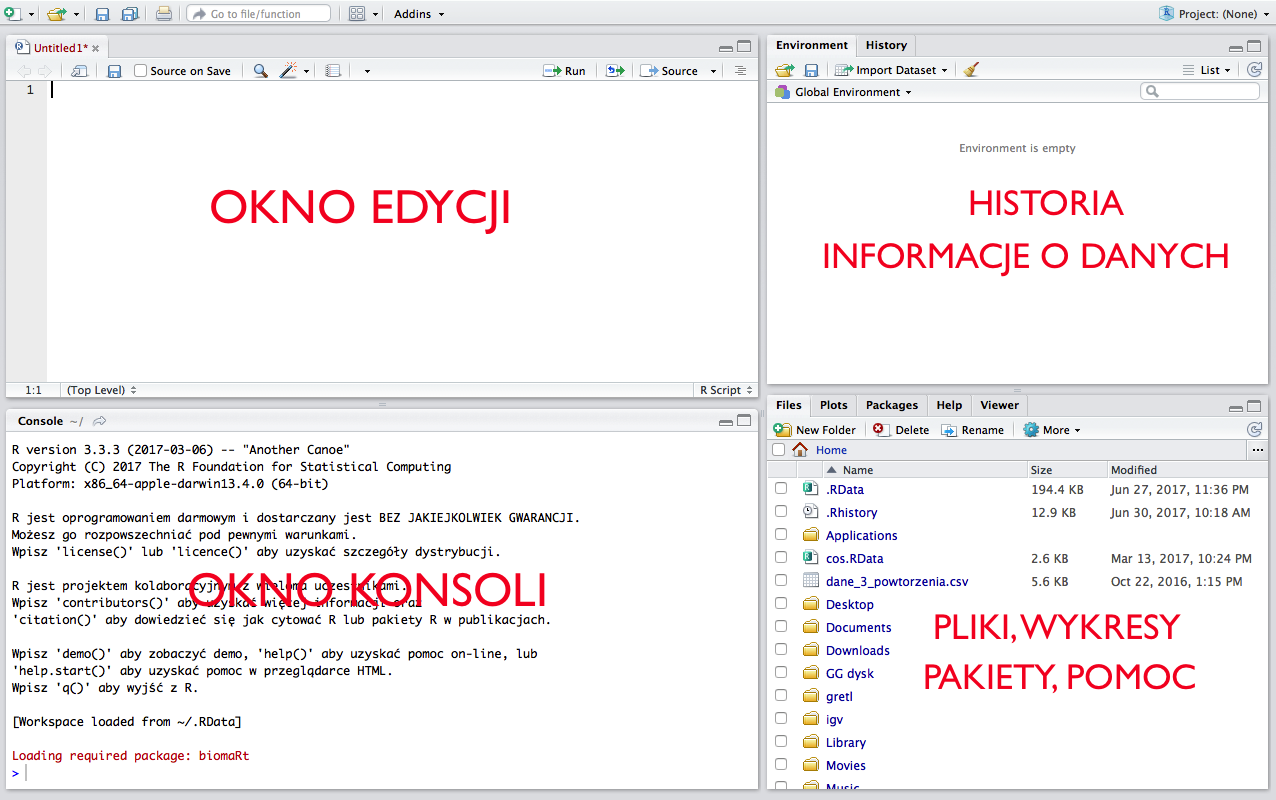
\includegraphics[width=0.99\linewidth]{images/RStudio} 

}

\caption{Przykładowy ekran RStudio}\label{fig:unnamed-chunk-2}
\end{figure}

Interfejs RStudio składa się z czterech okien. Lewe dolne okno jest
konsolą. Po znaku zachęty ``\textgreater{}'' możemy napisać polecenie
(komendę, skrypt) i po naciśnięciu klawisza ``enter'' polecenie to
zostanie wykonane, a wynik zostanie wyświetlony poniżej. Okno lewe górne
(okno edycji) służy do edycji skryptów, które można tworzyć, zmieniać,
zapisywać oraz wykonywać klikając na polecenie ``run''. Wyniki
realizacji poleceń wyświetlane są w lewym dolnym oknie, czyli oknie
konsoli. Okno prawe górne jest oknem zawierającym historię działania w
RStudio oraz przedstawiającym informacje o wprowadzonych danych.
Natomiast w prawym dolnym oknie znajdują się informacje o pakietach,
plikach, wyświetlane są rysunki oraz pomoc.

\vspace{0.8cm}

\textbf{Przydatne skróty klawiszowe w RStudio}

\begin{itemize}
\item
  uzupełnianie nazw funkcji i obiektów - `tab'
\item
  wyświetlanie kodu funkcji - klawisz F2
\item
  wyświetlanie pomocy na temat funkcji - klawisz F1
\item
  zamknięcie programu - ctrl+q
\item
  zamknięcie skryptu - ctrl+w
\end{itemize}

\textbf{Uwaga}

Należy najpierw zainstalować R, a następnie RStudio. Uruchamiamy tylko
RStudio.

\section{Pakiety}\label{pakiety}

Podczas instalacji R, instalowane są także systemowe pakiety
obliczeniowe (`system library'). W każdym momencie możemy zainstalować
dowolny pakiet korzystając z prawego dolnego okna RStudio. Należy w
zakładce ``Packages'' uruchomić polecenie ``Install'' i wpisać nazwę
pakietu. Natomiast informacje dotyczące pakietów można uzyskać na dwa
sposoby. Po pierwsze, w RStudio w prawym dolnym oknie wybierając
``Packages'' mamy spis wszystkich zainstalowanych pakietów. Drugi
sposób, to kolejno uruchamiamy:

\begin{enumerate}
\def\labelenumi{\arabic{enumi}.}
\tightlist
\item
  www.r-project.org
\item
  CRAN
\item
  np. ``\url{https://cloud.r-project.org/}''
\item
  ``Packages''.
\end{enumerate}

Po zainstalowaniu pakietu, można z niego korzystać (czyli stosować
polecenia w nim zawarte) dopiero po aktywowaniu pakietu poleceniem
library(), gdzie w nawiasach wpisana jest nazwa pakietu.

\section{Dokumentacja i szukanie
pomocy}\label{dokumentacja-i-szukanie-pomocy}

Materiały dla początkujących, a także zaawansowanych użytkowników R
dotyczące jego wykorzystania w podstawowej oraz zaawansowanej
statystyce, a także zastosowanie R w tworzeniu wykresów znajdują się na
różnych stronach internetowych, szczególnie na stronie
``www.r-project.org''. Są to artykuły, raporty oraz książki - także w
języku polskim. Natomiast pomoc najłatwiej można uzyskać wpisując w
oknie konsoli poszukiwane hasło poprzedzone znakiem zapytania lub
wpisując polecenie help(), gdzie w nawiasach wpisana jest nazwa hasła.
Treść pomocy wyświetlona zostanie w prawym dolnym oknie.

\section{Zadania do wykonania}\label{zadania-do-wykonania}

Zad. 1

Zainstaluj pakiet `agricolae' i przedstaw własności funkcji
`correlation'.

Zad. 2

Zainstaluj pakiet `agridat' i opisz dane `yates.oats'.

Zad. 3

Zainstaluj pakiet `openxlsx' i przedstaw informacje o funkcji
`read.xlsx'.

\chapter{Obliczenia w R}\label{obliczenia-w-r}

W programie R mamy nie tylko możliwość wykonywania zaawansowanych
obliczeń statystycznych, ale także możemy używać R do zwykłych działań
jako kalkulatora.

Polecenia w R można realizować na kilka sposobów. Dwa najprostsze są
następujące:

\begin{enumerate}
\def\labelenumi{\arabic{enumi}.}
\tightlist
\item
  W lewym górnym oknie RStudio (okno edycji) piszemy polecenie (kod,
  skrypt) i następnie wykonujemy polecenie ``Run'' (kursor wskazuje,
  który wiersz poleceń będzie wykonany, natomiast zaznaczony obszar
  wskazuje, które polecenia będą wykonane).
\item
  W lewym dolnym oknie RStudio (okno konsoli) po znaku zachęty
  ``\textgreater{}'' piszemy polecenie (kod, skrypt) i wykonujemy to
  polecenie naciskając klawisz ``enter''.
\end{enumerate}

\textbf{Uwagi}

\begin{enumerate}
\def\labelenumi{\arabic{enumi}.}
\tightlist
\item
  Realizacja wykonanych poleceń przedstawiana jest w lewym dolnym oknie
  RStudio (okno konsoli).
\item
  Po znaku ``\#'' występuje komentarz, który nie jest wykonywany.
\item
  Liczba rzeczywista przedstawiana jest za pomocą kropki, a nie
  przecinka (separatorem dziesietnym jest kropka, a nie przecinek).
\item
  Nazwy obiektów mogą zawierać duże i małe litery, przy czym wielkość
  znaków jest rozróżnialna.
\item
  Nazwy nie mogą się zaczynać od liczby oraz znaku `\_'.
\end{enumerate}

\section{Proste obliczenia
matematyczne}\label{proste-obliczenia-matematyczne}

\begin{table}[!ht]
\centering
\caption{Podstawowe funkcje i operatory w R}
\label{operatory}
\begin{tabular}{ccc}
\hline
Funkcja/Operator  & Opis jej działania  & Przykład użycia  \\ \hline
+, - , /, *                                                                                   & \begin{tabular}[c]{@{}c@{}}Dodawanie, odejmowanie, dzielenie, \\ mnożenie\end{tabular}                                                                                              & 2+3; 1-2; 4/2; 4*3                                              \\
sqrt(x), \textasciicircum      & Pierwiastkowanie, potęgowanie                                         & sqrt(4); 2\textasciicircum 4    \\
\begin{tabular}[c]{@{}c@{}}log(x), log10(x) \\ log(x, a)\\  log2(x) \\ exp(x)\end{tabular} & \begin{tabular}[c]{@{}c@{}}Logarytm naturalny (log), dziesiętny (log10) \\ Logarytm o podstawie a z liczby x \\ Logarytm o podstawie 2 \\ Funkcja wykładnicza $e^x$\end{tabular} & \begin{tabular}[c]{@{}c@{}}log(8); log10(4) \\log(6,9) \\ log2(5) \\ exp(3) \end{tabular}\\
sin(x), cos(x)    & Funkcje trygonometryczne sinus, cosinus z x  & sin(3*pi/4)  \\
round(x,a) & Zaokrąglenie x do a miejsc po przecinku & round(8.345,2) \\
x\%\%y                                                                                        & Reszta z dzielenia x przez y                                                                                                                                                        & 4\%\%3                                                          \\
x\%/\%y                                                                                       & Część całkowita z dzielenia x przez y                                                                                                                                               & 6\%/\%4                                                         \\
abs(x)                                                                                        & Wartość bezwzględna z x                                                                                                                                                             & abs(-4)                                                         \\ \hline                                                           
\end{tabular}
\end{table}

\textbf{Przykład 2.1}

W lewym górnym oknie RStudio (okno edycji) piszemy:

\begin{verbatim}
6+8 
\end{verbatim}

i wykonujemy polecenie ``Run''. Wówczas w lewym dolnym oknie RStudio
(okno konsoli) pojawi się:

\begin{verbatim}
> 6+8 
\end{verbatim}

\begin{verbatim}
[1] 14
\end{verbatim}

gdzie znak ``\textgreater{}'' jest znakiem zachęty, ``6+8'' jest
wykonanym poleceniem, ``{[}1{]}'' jest liczbą elementów wyjściowych,
natomiast ``14'' jest wynikiem realizacji polecenia wejściowego.

\textbf{Uwaga}

W prezentowanym manuskrypcie wszystkie polecenia, kody oraz skrypty
oznaczane są czcionką koloru czarnego i nazwane ``Kod w R''. Najlepiej
polecenia takie umieścić w lewym górnym oknie RStudio (okno edycji).
Natomiast wynik wykonania skryptu (po uruchomieniu poleceniem ``Run''),
przedstawiony jest w lewym dolnym oknie RStudio (okno konsoli) i nazwany
``Realizacja w R''.

\vspace{0.8cm}

\textbf{Przykład 2.2}

\textbf{Kod w R}

\begin{verbatim}
# Przykład 2.2 - proste obliczenia matematyczne
3+5 # dodawanie
4-6 # odejmowanie
8*7 # mnożenie
21/5 # dzielenie
5^3 # 5 do potęgi 3
sqrt(49) # pierwiastek kwadratowy z 49
49^(1/2) # pierwiastek kwadratowy z 49
(8)^(1/3) # pierwiastek trzeciego stopnia z 8
log(7) # logarytm naturalny z 7
log10(6) # logarytm o podstawie 10 z 6
log2(5) # logarytm o podstawie 2 z 5
log(4,5) # logarytm o podstawie 5 z 4
exp(3) # e do potęgi 3
sin(6.28) # sinus kąta 6.28 (w radianach), czyli kąta 360 stopni
cos(pi/2) # cosinus kąta pi/2 (w radianach), czyli kąta 90 stopni
\end{verbatim}

\vspace{0.8cm}

\textbf{Realizacja w R}

\begin{verbatim}
> # Przykład 2.2 - proste obliczenia matematyczne
> 3+5 # dodawanie
\end{verbatim}

\begin{verbatim}
[1] 8
\end{verbatim}

\begin{verbatim}
> 4-6 # odejmowanie
\end{verbatim}

\begin{verbatim}
[1] -2
\end{verbatim}

\begin{verbatim}
> 8*7 # mnożenie
\end{verbatim}

\begin{verbatim}
[1] 56
\end{verbatim}

\begin{verbatim}
> 21/5 # dzielenie
\end{verbatim}

\begin{verbatim}
[1] 4.2
\end{verbatim}

\begin{verbatim}
> 5^3 # 5 do potęgi 3
\end{verbatim}

\begin{verbatim}
[1] 125
\end{verbatim}

\begin{verbatim}
> sqrt(49) # pierwiastek kwadratowy z 49
\end{verbatim}

\begin{verbatim}
[1] 7
\end{verbatim}

\begin{verbatim}
> 49^(1/2) # pierwiastek kwadratowy z 49
\end{verbatim}

\begin{verbatim}
[1] 7
\end{verbatim}

\begin{verbatim}
> (8)^(1/3) # pierwiastek trzeciego stopnia z 8
\end{verbatim}

\begin{verbatim}
[1] 2
\end{verbatim}

\begin{verbatim}
> log(7) # logarytm naturalny z 7
\end{verbatim}

\begin{verbatim}
[1] 1.94591
\end{verbatim}

\begin{verbatim}
> log10(6) # logarytm o podstawie 10 z 6
\end{verbatim}

\begin{verbatim}
[1] 0.7781513
\end{verbatim}

\begin{verbatim}
> log2(5) # logarytm o podstawie 2 z 5
\end{verbatim}

\begin{verbatim}
[1] 2.321928
\end{verbatim}

\begin{verbatim}
> log(4,5) # logarytm o podstawie 5 z 4
\end{verbatim}

\begin{verbatim}
[1] 0.8613531
\end{verbatim}

\begin{verbatim}
> exp(3) # e do potęgi 3
\end{verbatim}

\begin{verbatim}
[1] 20.08554
\end{verbatim}

\begin{verbatim}
> sin(6.28) # sinus kąta 6.28 (w radianach), czyli kąta 360 stopni
\end{verbatim}

\begin{verbatim}
[1] -0.003185302
\end{verbatim}

\begin{verbatim}
> cos(pi/2) # cosinus kąta pi/2 (w radianach), czyli kąta 90 stopni
\end{verbatim}

\begin{verbatim}
[1] 6.123234e-17
\end{verbatim}

\vspace{0.8cm}

\textbf{Uwaga}

W R można zapisać różne działania w tej samej linii, ale muszą być
oddzielone średnikami.

\vspace{0.8cm}

\textbf{Przykład 2.3}

\textbf{Kod w R}

\begin{verbatim}
# Przykład 2.3 - obliczenia matematyczne
2+3; 1-2; 4/2; 4*3
\end{verbatim}

\vspace{0.8cm}

\textbf{Realizacja w R}

\begin{verbatim}
> # Przykład 2.3 - obliczenia matematyczne
> 2+3; 1-2; 4/2; 4*3
\end{verbatim}

\begin{verbatim}
[1] 5
\end{verbatim}

\begin{verbatim}
[1] -1
\end{verbatim}

\begin{verbatim}
[1] 2
\end{verbatim}

\begin{verbatim}
[1] 12
\end{verbatim}

\section{Zmienne}\label{zmienne}

W R operatorem przypisania jest znak ``='' lub ``\textless{}-''. W
manuskrypcie stosujemy znak ``=''.

\vspace{0.8cm}

\textbf{Przykład 2.4}

\textbf{Kod w R}

\begin{verbatim}
# Przykład 2.4 - operacje przypisania
x=4  # przypisanie zmiennej x wartości 4
x  # wyświetlenie wartości zmiennej x, czyli 4
imie = "Jan"
imie
nazwisko="Nowak"
nazwisko
\end{verbatim}

\textbf{Realizacja w R}

\begin{verbatim}
> # Przykład 2.4 - operacje przypisania
> x=4  # przypisanie zmiennej x wartości 4
> x  # wyświetlenie wartości zmiennej x, czyli 4
\end{verbatim}

\begin{verbatim}
[1] 4
\end{verbatim}

\begin{verbatim}
> imie = "Jan"
> imie
\end{verbatim}

\begin{verbatim}
[1] "Jan"
\end{verbatim}

\begin{verbatim}
> nazwisko="Nowak"
> nazwisko
\end{verbatim}

\begin{verbatim}
[1] "Nowak"
\end{verbatim}

\section{Wektory, macierze oraz ramki
danych}\label{wektory-macierze-oraz-ramki-danych}

\textbf{WEKTORY}

Podstawowa funkcja wykorzystywana w R w celu utworzenia wektora to
``\texttt{c()}'' od `concatenate' - powiązać. Przykładowo, gdy chcemy
utworzyć wektor o nazwie ``a'' z elementami 3 i 1 piszemy a=c(3,1).
Wektor musi posiadać elementy tylko jednego typu. Rozróżniamy
następujące wektory: wektor numeryczny, wektor znakowy oraz wektor
logiczny.

\vspace{0.8cm}

\textbf{Przykład 2.5}

\textbf{Kod w R}

\begin{verbatim}
# Przykład 2.5 - wektory
 # wektor numeryczny
a = c(3, 5, 7, 9, 11) 
a
#  wektor znakowy, znak w cudzysłowiu ""
dni = c("wtorek", "czwartek", "sobota", "niedziela")  
dni
# wektor logiczny
c = c(TRUE,TRUE,TRUE,FALSE,TRUE,FALSE) 
c
\end{verbatim}

\vspace{0.8cm}

\textbf{Realizacja w R}

\begin{verbatim}
> # Przykład 2.5 - wektory
>  # wektor numeryczny
> a = c(3, 5, 7, 9, 11) 
> a
\end{verbatim}

\begin{verbatim}
[1]  3  5  7  9 11
\end{verbatim}

\begin{verbatim}
> #  wektor znakowy, znak w cudzysłowiu ""
> dni = c("wtorek", "czwartek", "sobota", "niedziela")  
> dni
\end{verbatim}

\begin{verbatim}
[1] "wtorek"    "czwartek"  "sobota"    "niedziela"
\end{verbatim}

\begin{verbatim}
> # wektor logiczny
> c = c(TRUE,TRUE,TRUE,FALSE,TRUE,FALSE) 
> c
\end{verbatim}

\begin{verbatim}
[1]  TRUE  TRUE  TRUE FALSE  TRUE FALSE
\end{verbatim}

Przykładowe metody tworzenia wektorów znajdują się w Tablicy 2.2.

\begin{table}[!ht]
\centering
\caption{Przykładowe funkcje tworzenia wektorów}
\label{cos}
\begin{tabular}{ccc}
\hline
Funkcja/Operator                                                             & \begin{tabular}[c]{@{}c@{}}Przykład\\ {[}wynik{]}\end{tabular}                           & Opis                                                                                                                          \\ \hline
:                                                                         & \begin{tabular}[c]{@{}c@{}}1:3\\ {[}1,2,3{]}\end{tabular}                              & Tworzy sekwencje od : do                                                                                                      \\ \hline
seq(from=x,to=y,by=z)                                                     & \begin{tabular}[c]{@{}c@{}}seq(from=0,to=8,by=2)\\ {[}0,2,4,6,8{]}\end{tabular}          & \begin{tabular}[c]{@{}c@{}}Tworzy regularne sekwencje \\ od 0 do 8 co 2\end{tabular}                                          \\ \hline
\begin{tabular}[c]{@{}c@{}}seq(from=x,to=y, \\ length.out=z)\end{tabular} & \begin{tabular}[c]{@{}c@{}}seq(from=0,to=10,\\ length.out=3)\\ {[}0,5,10{]}\end{tabular} & \begin{tabular}[c]{@{}c@{}}Tworzy\\ regularne sekwencje \\ od 0 do 10 co 3 liczbach\end{tabular}                               \\ \hline
\begin{tabular}[c]{@{}c@{}}rep(x),\\ rep(x,y)\end{tabular}                & \begin{tabular}[c]{@{}c@{}}rep(3); rep(3,4)\\ {[}3{]}; {[}3,3,3,3{]}\end{tabular}        & \begin{tabular}[c]{@{}c@{}}Pierwszy argument oznacza \\ co ma być powtórzone\\ drugi ile razy (domyślnie jest 1)\end{tabular} \\ \hline
rep(x,length.out=y)                                                       & \begin{tabular}[c]{@{}c@{}}rep(1:2,length.out=4)\\ {[}1,2,1,2{]}\end{tabular}            & \begin{tabular}[c]{@{}c@{}}Powtórzona sekwencja liczb \\ 1 i 2 o długości 4\end{tabular}                                      \\ \hline
rep(x,each=y)                                                             & \begin{tabular}[c]{@{}c@{}}rep(3:1,each=2)\\ {[}3,3,2,2,1,1{]}\end{tabular}              & \begin{tabular}[c]{@{}c@{}}Każda\\ cyfra z sekwencji 3:1 \\ powtórzona 2 razy\end{tabular}                                    \\ \hline
\end{tabular}
\end{table}

\vspace{0.8cm}

\textbf{Przykład 2.6}

\textbf{Kod w R}

\begin{verbatim}
# Przykład 2.6 - operacje na wektorach
a = c(1,3,5) # określenie wektora a
a
b=c(3:14) # określenie wektora b
b
# łączymy wektory a i b
ab = c(a,b)
ab
# zastępujemy liczby z pozycji 6,7,...,10 innymi liczbami
ab[6:10] = c(0,-6,-3,-1,-5) 
ab
# Alternatywne metody tworzenia wektorów:
rep(c(1,2), times=3) # powtarzamy wektor (1,2) - 3 razy
rep(c(1,2), each=3)  # powtarzamy elementy wektora (1,2) - 3 razy
seq(from=1, to=10, by=2 ) # tworzymy sekwencję liczb (od 1 do 10 co 2)
\end{verbatim}

\vspace{0.8cm} \textbf{Realizacja w R}

\begin{verbatim}
> # Przykład 2.6 - operacje na wektorach
> a = c(1,3,5) # określenie wektora a
> a
\end{verbatim}

\begin{verbatim}
[1] 1 3 5
\end{verbatim}

\begin{verbatim}
> b=c(3:14) # określenie wektora b
> b
\end{verbatim}

\begin{verbatim}
 [1]  3  4  5  6  7  8  9 10 11 12 13 14
\end{verbatim}

\begin{verbatim}
> # łączymy wektory a i b
> ab = c(a,b)
> ab
\end{verbatim}

\begin{verbatim}
 [1]  1  3  5  3  4  5  6  7  8  9 10 11 12 13 14
\end{verbatim}

\begin{verbatim}
> # zastępujemy liczby z pozycji 6,7,...,10 innymi liczbami
> ab[6:10] = c(0,-6,-3,-1,-5) 
> ab
\end{verbatim}

\begin{verbatim}
 [1]  1  3  5  3  4  0 -6 -3 -1 -5 10 11 12 13 14
\end{verbatim}

\begin{verbatim}
> # Alternatywne metody tworzenia wektorów:
> rep(c(1,2), times=3) # powtarzamy wektor (1,2) - 3 razy
\end{verbatim}

\begin{verbatim}
[1] 1 2 1 2 1 2
\end{verbatim}

\begin{verbatim}
> rep(c(1,2), each=3)  # powtarzamy elementy wektora (1,2) - 3 razy
\end{verbatim}

\begin{verbatim}
[1] 1 1 1 2 2 2
\end{verbatim}

\begin{verbatim}
> seq(from=1, to=10, by=2 ) # tworzymy sekwencję liczb (od 1 do 10 co 2)
\end{verbatim}

\begin{verbatim}
[1] 1 3 5 7 9
\end{verbatim}

\vspace{0.8cm} \textbf{Odwoływanie się do elementów wektora:}

\begin{enumerate}
\def\labelenumi{\alph{enumi})}
\item
  x{[}1:2{]} - odwołanie się do 1 i 2 elementu wektora x
\item
  x{[}c(2,4){]} - odwołanie się do 2 i 4 elementu wektora x
\item
  x{[}-c(2,3){]} - wektor x bez 2 i 3 elementu
\item
  x{[}x\textgreater{}6{]} - podzbiór wektora x: wyświetlane są tylko te
  wartości wektora x, które są większe od 6
\end{enumerate}

\vspace{0.8cm}

\textbf{Przykład 2.7}

\textbf{Kod w R}

\begin{verbatim}
# Przykład 2.7 - odwoływanie się do elementów wektora
x = 1:7  # określenie wektora x
x
x[5]  # 5-ty element wektora x
x[-1]  # wszystkie elementy oprócz pierwszego elementu wektora x
x[2:6]  # od 2-go do 6-go elementu wektora x
x[c(2, 4)]  # 2-gi i 4-ty element wektora x
x[x < 4]  # wszystkie elementy wektora x mniejsze od 4
\end{verbatim}

\newpage

\textbf{Realizacja w R}

\begin{verbatim}
> # Przykład 2.7 - odwoływanie się do elementów wektora
> x=1:7 # określenie wektora x
> x
\end{verbatim}

\begin{verbatim}
[1] 1 2 3 4 5 6 7
\end{verbatim}

\begin{verbatim}
> x[5]           # 5-ty element wektora x
\end{verbatim}

\begin{verbatim}
[1] 5
\end{verbatim}

\begin{verbatim}
> x[-1]          # wszystkie elementy oprócz pierwszego elementu wektora x
\end{verbatim}

\begin{verbatim}
[1] 2 3 4 5 6 7
\end{verbatim}

\begin{verbatim}
> x[2:6]         # od 2-go do 6-go elementu wektora x
\end{verbatim}

\begin{verbatim}
[1] 2 3 4 5 6
\end{verbatim}

\begin{verbatim}
> x[c(2,4)]      # 2-gi i 4-ty element wektora x
\end{verbatim}

\begin{verbatim}
[1] 2 4
\end{verbatim}

\begin{verbatim}
> x[x < 4]       # wszystkie elementy wektora x mniejsze od 4
\end{verbatim}

\begin{verbatim}
[1] 1 2 3
\end{verbatim}

\vspace{0.8cm} \textbf{Podstawowe operacje na wektorach: }

\texttt{x} jest wektorem liczbowym

\texttt{length(x)} - liczba elementów wektora \texttt{x}

\texttt{min(x)}, \texttt{max(x)}, \texttt{range(x)} - minimum, maximum,
rozstęp

\texttt{sum(x)}, \texttt{prod(x)} - suma i iloczyn elementów

\texttt{mean(x)}, \texttt{median(x)} - średnia arytmetyczna i mediana

\texttt{var(x)}, \texttt{sd(x)} - wariancja i odchylenie standardowe

\texttt{IQR(x)} - zakres międzykwartylowy

\texttt{sort(x)} - posortowane elementy w kolejności rosnącej

\texttt{summary(x)} - podstawowe statystyki: min, max, średnia, mediana,
kwartyle

\vspace{0.8cm} \textbf{Przykład 2.8} (Kala 2005, s. 26)

Obserwowano plonowanie 30 krzaków pomidorów ``New Yorker'' i otrzymano
następujące wielkości plonów (w kg): 1.52, 1.57, 1.30, 1.62, 1.55, 1.70,
2.05, 1.64, 1.95, 1.80, 1.76, 1.40, 1.92, 2.20, 1.57, 1.59, 1.27, 1.79,
1.29, 1.84, 1.77, 1.72, 1.53, 1.32, 1.69, 1.95, 1.75, 1.08, 1.70, 1.45.

Wyznaczyć wartość minimalną i maksymalną, rozstęp, sumę i iloczyn
elementów, średnią arytmetyczną i medianę, wariancję i odchylenie
standardowe. Następnie rosnąco posortować wszystkie elementy oraz
wykonać polecenie ``summary''.

\vspace{0.8cm}

\textbf{Kod w R}

\begin{verbatim}
# Przykład 2.8 - (Kala 2005, s.26)
# Przygotowanie danych
y = c(1.52, 1.57, 1.30, 1.62, 1.55, 1.70, 2.05, 1.64, 1.95, 1.80, 1.76, 1.40,
      1.92, 2.20, 1.57, 1.59, 1.27, 1.79, 1.29, 1.84, 1.77, 1.72, 1.53, 1.32,
      1.69, 1.95, 1.75, 1.08, 1.70, 1.45) 
# wyświetlanie zawartości y
y
# wykonanie obliczeń
min(y)  # wartość minimalna 
max(y)  # wartość maksymalna
range(y)  # wartość min i max
length(y) # liczba elementów
sum(y)  # suma elementów 
prod(y)  # iloczyn elementów 
var(y)  # wariancja
sd(y)  # odchylenie standardowe
sort(y) # sortowanie elementów (szereg pozycyjny)
summary(y) # wartości wybranych statystyk
\end{verbatim}

\vspace{0.8cm} \textbf{Realizacja w R}

\begin{verbatim}
> # Przykład 2.8 - (Kala 2005, s.26)
> # Przygotowanie danych
> y = c(1.52, 1.57, 1.30, 1.62, 1.55, 1.70, 2.05, 1.64, 1.95, 1.80, 1.76, 1.40,
+       1.92, 2.20, 1.57, 1.59, 1.27, 1.79, 1.29, 1.84, 1.77, 1.72, 1.53, 1.32,
+       1.69, 1.95, 1.75, 1.08, 1.70, 1.45) 
> # wyświetlanie zawartości y
> y
\end{verbatim}

\begin{verbatim}
 [1] 1.52 1.57 1.30 1.62 1.55 1.70 2.05 1.64 1.95 1.80 1.76 1.40 1.92 2.20
[15] 1.57 1.59 1.27 1.79 1.29 1.84 1.77 1.72 1.53 1.32 1.69 1.95 1.75 1.08
[29] 1.70 1.45
\end{verbatim}

\begin{verbatim}
> # wykonanie obliczeń
> min(y)  # wartość minimalna 
\end{verbatim}

\begin{verbatim}
[1] 1.08
\end{verbatim}

\begin{verbatim}
> max(y)  # wartość maksymalna
\end{verbatim}

\begin{verbatim}
[1] 2.2
\end{verbatim}

\begin{verbatim}
> range(y)  # wartość min i max
\end{verbatim}

\begin{verbatim}
[1] 1.08 2.20
\end{verbatim}

\begin{verbatim}
> length(y) # liczba elementów
\end{verbatim}

\begin{verbatim}
[1] 30
\end{verbatim}

\begin{verbatim}
> sum(y)  # suma elementów 
\end{verbatim}

\begin{verbatim}
[1] 49.29
\end{verbatim}

\begin{verbatim}
> prod(y)  # iloczyn elementów 
\end{verbatim}

\begin{verbatim}
[1] 2068140
\end{verbatim}

\begin{verbatim}
> var(y)  # wariancja
\end{verbatim}

\begin{verbatim}
[1] 0.06315966
\end{verbatim}

\begin{verbatim}
> sd(y)  # odchylenie standardowe
\end{verbatim}

\begin{verbatim}
[1] 0.2513158
\end{verbatim}

\begin{verbatim}
> sort(y) # sortowanie elementów (szereg pozycyjny)
\end{verbatim}

\begin{verbatim}
 [1] 1.08 1.27 1.29 1.30 1.32 1.40 1.45 1.52 1.53 1.55 1.57 1.57 1.59 1.62
[15] 1.64 1.69 1.70 1.70 1.72 1.75 1.76 1.77 1.79 1.80 1.84 1.92 1.95 1.95
[29] 2.05 2.20
\end{verbatim}

\begin{verbatim}
> summary(y) # wartości wybranych statystyk
\end{verbatim}

\begin{verbatim}
   Min. 1st Qu.  Median    Mean 3rd Qu.    Max. 
  1.080   1.523   1.665   1.643   1.785   2.200 
\end{verbatim}

\vspace{0.8cm} \textbf{MACIERZE}

\vspace{0.8cm} \textbf{Macierz} - zbiór elementów tego samego typu o
strukturze wierszy i kolumn.

Przykład macierzy o 3 wierszach i 5 kolumnach:

\[
  \begin{pmatrix}
2 &  3 & 7&  5 & 1 \\ 
7 & 9 & 1 & 4 & 0 \\
8 & 2 & 6 & 3 & 7 \\
\end{pmatrix}
\]

Funkcją tworzącą macierz jest

\begin{center}
\texttt{matrix(data, nrow, ncol, byrow)}
\end{center}

gdzie:

\texttt{data} - dane, które chcemy przedstawić w formie macierzy,

\texttt{nrow} - liczba wierszy,

\texttt{ncol} - liczba kolumn,

\texttt{byrow} - jeśli byrow=TRUE, to macierz tworzona jest wierszami
(domyślnie byrow=FALSE)

\vspace{0.8cm}

\textbf{Przykład 2.9}

\textbf{Kod w R}

\begin{verbatim}
# Przykład 2.9 - tworzenie macierzy
# macierz o 3 wierszach tworzona kolumnami
mat1 = matrix(c(1,3,5,7,9,11,13,15,18,21,23,25),  nrow = 3)  
mat1
# macierz o 3 kolumnach tworzona kolumnami
mat2 = matrix(c(1,3,5,7,9,11,13,15,18,21,23,25),  ncol = 3)  
mat2
# macierz o 3 wierszach i 2 kolumnach
mat3 = matrix(1:6,3,2)  
mat3
\end{verbatim}

\vspace{0.8cm} \textbf{Realizacja w R}

\begin{verbatim}
> # Przykład 2.9 - tworzenie macierzy
> # macierz o 3 wierszach
> mat1 = matrix(c(1,3,5,7,9,11,13,15,18,21,23,25),  nrow = 3)  
> mat1
\end{verbatim}

\begin{verbatim}
     [,1] [,2] [,3] [,4]
[1,]    1    7   13   21
[2,]    3    9   15   23
[3,]    5   11   18   25
\end{verbatim}

\begin{verbatim}
> # macierz o 3 kolumnach
> mat2 = matrix(c(1,3,5,7,9,11,13,15,18,21,23,25),  ncol = 3)  
> mat2
\end{verbatim}

\begin{verbatim}
     [,1] [,2] [,3]
[1,]    1    9   18
[2,]    3   11   21
[3,]    5   13   23
[4,]    7   15   25
\end{verbatim}

\begin{verbatim}
> # macierz o 3 wierszach i 2 kolumnach
> mat3 = matrix(1:6,3,2)    
> mat3
\end{verbatim}

\begin{verbatim}
     [,1] [,2]
[1,]    1    4
[2,]    2    5
[3,]    3    6
\end{verbatim}

\vspace{0.8cm}

\textbf{Przykład 2.10}

\textbf{Kod w R}

\begin{verbatim}
# Przykład 2.10 - alternatywne metody tworzenia macierzy
macierz1 = matrix(seq(1:8), nrow = 4)
macierz1
macierz2 = matrix(seq(1:8), nrow = 4, byrow = TRUE)
macierz2
# macierz diagonalna
macdiag1 = diag(1:5)
macdiag1
# macierz jednostkowa
macdiag2 = diag(4)
macdiag2
\end{verbatim}

\vspace{0.8cm} \textbf{Realizacja w R}

\begin{verbatim}
> # Przykład 2.10 - alternatywne metody tworzenia macierzy
> macierz1 = matrix(seq(1:8), nrow = 4)
> macierz1
\end{verbatim}

\begin{verbatim}
     [,1] [,2]
[1,]    1    5
[2,]    2    6
[3,]    3    7
[4,]    4    8
\end{verbatim}

\begin{verbatim}
> macierz2 = matrix(seq(1:8),  nrow = 4, byrow=TRUE)
> macierz2
\end{verbatim}

\begin{verbatim}
     [,1] [,2]
[1,]    1    2
[2,]    3    4
[3,]    5    6
[4,]    7    8
\end{verbatim}

\begin{verbatim}
> # macierz diagonalna
> macdiag1=diag(1:5)      
> macdiag1
\end{verbatim}

\begin{verbatim}
     [,1] [,2] [,3] [,4] [,5]
[1,]    1    0    0    0    0
[2,]    0    2    0    0    0
[3,]    0    0    3    0    0
[4,]    0    0    0    4    0
[5,]    0    0    0    0    5
\end{verbatim}

\begin{verbatim}
> # macierz jednostkowa
> macdiag2=diag(4)      
> macdiag2
\end{verbatim}

\begin{verbatim}
     [,1] [,2] [,3] [,4]
[1,]    1    0    0    0
[2,]    0    1    0    0
[3,]    0    0    1    0
[4,]    0    0    0    1
\end{verbatim}

\vspace{0.8cm}

\textbf{Odwoływanie się do elementów macierzy:}

\begin{enumerate}
\def\labelenumi{\alph{enumi})}
\item
  A{[}2,3{]} - element z drugiego wiersza i trzeciej kolumny macierzy A
\item
  A{[}2, {]} - drugi wiersz macierzy A
\item
  A{[} ,3{]} - trzecia kolumna macierzy A
\item
  A{[} ,c(1,3){]} - pierwsza i trzecia kolumna macierzy A
\end{enumerate}

\textbf{Przykład 2.11}

\textbf{Kod w R}

\begin{verbatim}
# Przykład 2.11 - odwoływanie się do elementów macierzy
dane1 = matrix(seq(1:12),nrow = 3) # tworzenie macierzy dane1
dane1 # wyświetlenie zawartości macierzy dane1
dane1[1,2]  # element z pierwszego wiersza i drugiej kolumny macierzy dane1
dane1[2,]  # drugi wiersz macierzy dane1
dane1[,3]  # trzecia kolumna macierzy dane1
dane1[ ,c(1,4)]  # pierwsza i czwarta kolumna macierzy dane1
dane1[c(1,3),]  # pierwszy i trzeci wiersz macierzy dane1
\end{verbatim}

\vspace{0.8cm}

\textbf{Realizacja w R}

\begin{verbatim}
> # Przykład 2.11 - odwoływanie się do elementów macierzy
> dane1 = matrix(seq(1:12),  nrow = 3) # tworzenie macierzy dane1
> dane1 # wyświetlenie zawartości macierzy dane1
\end{verbatim}

\begin{verbatim}
     [,1] [,2] [,3] [,4]
[1,]    1    4    7   10
[2,]    2    5    8   11
[3,]    3    6    9   12
\end{verbatim}

\begin{verbatim}
> dane1[1,2]  # element z pierwszego wiersza i drugiej kolumny macierzy dane1
\end{verbatim}

\begin{verbatim}
[1] 4
\end{verbatim}

\begin{verbatim}
> dane1[2,]  # drugi wiersz macierzy dane1
\end{verbatim}

\begin{verbatim}
[1]  2  5  8 11
\end{verbatim}

\begin{verbatim}
> dane1[,3]  # trzecia kolumna macierzy dane1
\end{verbatim}

\begin{verbatim}
[1] 7 8 9
\end{verbatim}

\begin{verbatim}
> dane1[ ,c(1,4)]  # pierwsza i czwarta kolumna macierzy dane1
\end{verbatim}

\begin{verbatim}
     [,1] [,2]
[1,]    1   10
[2,]    2   11
[3,]    3   12
\end{verbatim}

\begin{verbatim}
> dane1[c(1,3),]  # pierwszy i trzeci wiersz macierzy dane1
\end{verbatim}

\begin{verbatim}
     [,1] [,2] [,3] [,4]
[1,]    1    4    7   10
[2,]    3    6    9   12
\end{verbatim}

\vspace{0.8cm}

\textbf{Podstawowe operacje na macierzach: }

\texttt{dim(A)} - wymiar macierzy A

\texttt{A\%*\%B} - iloczyn macierzy A i B

\texttt{t(A)} - transpozycja macierzy A

\texttt{det(A)} - wyznacznik macierzy A

\texttt{solve(A)} - macierz odwrotna do macierzy A

\texttt{ncol(A), nrow(A)} - liczba kolumn, wierszy macierzy A

\texttt{colnames(A), rownames(A)} - nazwy kolumn, wierszy macierzy A

\texttt{colSums(A), rowSums(A)} - sumy kolumn, wierszy macierzy A

\texttt{colMeans(A), rowMeans(A)} - wartości średnie dla kolumn, wierszy
macierzy A

\texttt{diag(A)} - wektor o elementach z przekątnej macierzy A

\vspace{0.8cm}

\textbf{Przykład 2.12}

\textbf{Kod w R}

\begin{verbatim}
# Przykład 2.12 - operacje na macierzach
macierz1
dim(macierz1) # wymiar macierzy
t(macierz1) # transpozycja macierzy
\end{verbatim}

\vspace{0.8cm} \textbf{Realizacja w R}

\begin{verbatim}
> # Przykład 2.12 - operacje na macierzach
> macierz1
\end{verbatim}

\begin{verbatim}
     [,1] [,2]
[1,]    1    5
[2,]    2    6
[3,]    3    7
[4,]    4    8
\end{verbatim}

\begin{verbatim}
> dim(macierz1) # wymiar macierzy
\end{verbatim}

\begin{verbatim}
[1] 4 2
\end{verbatim}

\begin{verbatim}
> t(macierz1) # transpozycja macierzy
\end{verbatim}

\begin{verbatim}
     [,1] [,2] [,3] [,4]
[1,]    1    2    3    4
[2,]    5    6    7    8
\end{verbatim}

\vspace{0.8cm} \textbf{Przykład 2.13}

\textbf{Kod w R}

\begin{verbatim}
# Przykład 2.13 - mnożenie macierzy
A=matrix(c(1,2,3,4,5,6), nrow=2)
A
B=matrix(c(9,8,7,6,5,4,3,2,1), nrow=3)
B
C=A%*%B 
C
\end{verbatim}

\vspace{0.8cm} \textbf{Realizacja w R}

\begin{verbatim}
> # Przykład 2.13 - mnożenie macierzy
> A=matrix(c(1,2,3,4,5,6), nrow=2)
> A
\end{verbatim}

\begin{verbatim}
     [,1] [,2] [,3]
[1,]    1    3    5
[2,]    2    4    6
\end{verbatim}

\begin{verbatim}
> B=matrix(c(9,8,7,6,5,4,3,2,1), nrow=3)
> B
\end{verbatim}

\begin{verbatim}
     [,1] [,2] [,3]
[1,]    9    6    3
[2,]    8    5    2
[3,]    7    4    1
\end{verbatim}

\begin{verbatim}
> C=A%*%B 
> C
\end{verbatim}

\begin{verbatim}
     [,1] [,2] [,3]
[1,]   68   41   14
[2,]   92   56   20
\end{verbatim}

\vspace{0.8cm}

\textbf{Przykład 2.14}

\textbf{Kod w R}

\begin{verbatim}
# Przykład 2.14 - dalsze operacje na macierzach
rowSums(B) # sumy dla wierszy macierzy B
rowMeans(B) # średnie arytmetyczne dla wierszy macierzy B
colSums(A) # sumy dla kolumn macierzy A
colMeans(A) # średnie arytmetyczne dla kolumn macierzy A
\end{verbatim}

\vspace{0.8cm}

\textbf{Realizacja w R}

\begin{verbatim}
> # Przykład 2.14 - dalsze operacje na macierzach
> rowSums(B) # sumy dla wierszy macierzy B
\end{verbatim}

\begin{verbatim}
[1] 18 15 12
\end{verbatim}

\begin{verbatim}
> rowMeans(B) # średnie arytmetyczne dla wierszy macierzy B
\end{verbatim}

\begin{verbatim}
[1] 6 5 4
\end{verbatim}

\begin{verbatim}
> colSums(A) # sumy dla kolumn macierzy A
\end{verbatim}

\begin{verbatim}
[1]  3  7 11
\end{verbatim}

\begin{verbatim}
> colMeans(A) # średnie arytmetyczne dla kolumn macierzy A
\end{verbatim}

\begin{verbatim}
[1] 1.5 3.5 5.5
\end{verbatim}

\vspace{0.8cm} \textbf{Przykład 2.15}

\textbf{Kod w R}

\begin{verbatim}
# Przykład 2.15 - wyznacznik i odwrotność macierzy 
D=matrix(c(1,3,5,1,2,3,7,8,1), nrow=3)  
D
wyznacznik=det(D)  # wyznacznik macierzy D
wyznacznik
D1=solve(D)  # macierz odwrotna do macierzy D
D1
\end{verbatim}

\vspace{0.8cm} \textbf{Realizacja w R}

\begin{verbatim}
> # Przykład 2.15 -  wyznacznik i odwrotność macierzy
> D=matrix(c(1,3,5,1,2,3,7,8,1), nrow=3)  # tworzenie macierzy D
> D
\end{verbatim}

\begin{verbatim}
     [,1] [,2] [,3]
[1,]    1    1    7
[2,]    3    2    8
[3,]    5    3    1
\end{verbatim}

\begin{verbatim}
> wyznacznik=det(D)  # wyznacznik macierzy D
> wyznacznik
\end{verbatim}

\begin{verbatim}
[1] 8
\end{verbatim}

\begin{verbatim}
> D1=solve(D)  # macierz odwrotna do macierzy D
> D1
\end{verbatim}

\begin{verbatim}
       [,1]  [,2]   [,3]
[1,] -2.750  2.50 -0.750
[2,]  4.625 -4.25  1.625
[3,] -0.125  0.25 -0.125
\end{verbatim}

\vspace{0.8cm} \textbf{Przykład 2.16}

\textbf{Kod w R}

\begin{verbatim}
# Przykład 2.16 - rozwiązywanie układu równań
w=c(3,1,5)  # wektor wyrazów wolnych
w
roz=solve(D,w)  # rozwiązanie układu równań postaci Dx=w, D - macierz układu
roz
\end{verbatim}

\newpage

\textbf{Realizacja w R}

\begin{verbatim}
> # Przykład 2.16 - rozwiązywanie układu równań
> w=c(3,1,5)  # wektor wyrazów wolnych
> w
\end{verbatim}

\begin{verbatim}
[1] 3 1 5
\end{verbatim}

\begin{verbatim}
> roz=solve(D,w)  # rozwiązanie układu równań postaci Dx=w, D - macierz układu
> roz
\end{verbatim}

\begin{verbatim}
[1] -9.50 17.75 -0.75
\end{verbatim}

\vspace{0.8cm}

\textbf{RAMKA DANYCH}

\textbf{Ramka danych} - zbiór elementów o strukturze wierszy i kolumn,
gdzie kolumny mogą być różnego typu.

Funkcją tworzącą ramkę danych jest `data.frame'.

\vspace{0.8cm} \textbf{Przykład 2.17}

\textbf{Kod w R}

\begin{verbatim}
# Przykład 2.17 - tworzenie ramki danych
dawki=c("d0", "d20", "d50", "d100")
odmiany=c("K", "M", "P", "S")
plon=c(6.1, 5.4, 6.5, 6.3)
roslina=data.frame(Odmiany=odmiany, Dawki=dawki, Plon=plon)
roslina
\end{verbatim}

\newpage

\textbf{Realizacja w R}

\begin{verbatim}
> # Przykład 2.17 - tworzenie ramki danych
> dawki=c("d0", "d20", "d50", "d100")
> odmiany=c("K", "M", "P", "S")
> plon=c(6.1, 5.4, 6.5, 6.3)
> roslina=data.frame(Odmiany=odmiany, Dawki=dawki, Plon=plon)
> roslina
\end{verbatim}

\begin{verbatim}
  Odmiany Dawki Plon
1       K    d0  6.1
2       M   d20  5.4
3       P   d50  6.5
4       S  d100  6.3
\end{verbatim}

\vspace{0.8cm}

\textbf{Odwoływanie się do elementów z ramki danych:}

\begin{enumerate}
\def\labelenumi{\alph{enumi})}
\item
  roslina{[}1:3,1{]} - pierwsze trzy elementy pierwszej kolumny
\item
  roslina{[}1:2,`Odmiany'{]} - pierwsze dwa elementy kolumny o nazwie
  `Odmiany'
\item
  roslina\$Plon - wszystkie elementy z kolumny `Plon'
\item
  roslina\$Plon{[}1:2{]} - pierwsze dwa elementy z kolumny o nazwie
  `Plon'
\end{enumerate}

\vspace{0.4cm} \textbf{Przykład 2.18}

W R można korzystać z gotowych zbiorów danych. Przykładowe dane o nazwie
`iris' oraz `trees' użyte zostaną w dalszej części rozdziału.

\textbf{Kod w R}

\begin{verbatim}
# Przykład 2.18 - odwoływanie się do elementów ramki danych
# przykładowa ramka danych
data(iris) # załadowanie danych iris
head(iris) # wyświetlenie pierwszych elementów ze zbioru iris
iris[1:10,1] # pierwsze dziesięć elementów z pierwszej kolumny
iris[1:10,'Sepal.Length'] # lub równoznacznie
iris$Sepal.Length[1:10] # lub równoznacznie
\end{verbatim}

\vspace{0.8cm} \textbf{Realizacja w R}

\begin{verbatim}
> # Przykład 2.18 - odwoływanie się do elementów ramki danych
> # przykładowa ramka danych
> data(iris) # załadowanie danych iris
> head(iris) # wyświetlenie pierwszych elementów ze zbioru iris
\end{verbatim}

\begin{verbatim}
  Sepal.Length Sepal.Width Petal.Length Petal.Width Species
1          5.1         3.5          1.4         0.2  setosa
2          4.9         3.0          1.4         0.2  setosa
3          4.7         3.2          1.3         0.2  setosa
4          4.6         3.1          1.5         0.2  setosa
5          5.0         3.6          1.4         0.2  setosa
6          5.4         3.9          1.7         0.4  setosa
\end{verbatim}

\begin{verbatim}
> iris[1:10,1] # pierwsze dziesięć elementów z pierwszej kolumny
\end{verbatim}

\begin{verbatim}
 [1] 5.1 4.9 4.7 4.6 5.0 5.4 4.6 5.0 4.4 4.9
\end{verbatim}

\begin{verbatim}
> iris[1:10,'Sepal.Length'] # lub równoznacznie
\end{verbatim}

\begin{verbatim}
 [1] 5.1 4.9 4.7 4.6 5.0 5.4 4.6 5.0 4.4 4.9
\end{verbatim}

\begin{verbatim}
> iris$Sepal.Length[1:10] # lub równoznacznie
\end{verbatim}

\begin{verbatim}
 [1] 5.1 4.9 4.7 4.6 5.0 5.4 4.6 5.0 4.4 4.9
\end{verbatim}

\vspace{0.8cm}

\textbf{Podstawowe operacje na ramkach danych: }

\texttt{head()} - wyświetla pierwsze rekordy

\texttt{tail()} - wyświetla ostatnie rekordy

\texttt{attach()} - pozwala odnosić się do nazw zmiennych znajdujących
się bezpośrednio w danych

\texttt{detach()} - likwiduje możliwość bezpośredniego odnoszenia się do
zmiennych

\texttt{str()} - wyświetla informacje o obiekcie

\texttt{table()} - tabela z liczbą wystąpień danego czynnika lub
kombinacji czynników

\texttt{subset()} - określa podzbiór danego zbioru, spełniający
określone warunki

\texttt{by()} - stosuje określoną funkcję do zadanego podzbioru danych

\vspace{0.8cm} \textbf{Przykład 2.19}

\textbf{Kod w R}

\begin{verbatim}
# Przykład 2.19 - operacje na ramkach danych
data(trees)
head(trees)
attach(trees)
Girth
str(trees)
# tworzenie nowej ramki danych o nazwie 'ankieta'
ankieta = data.frame(odpowiedzi = c("T", "N", "T", "T", "N", "X", "N", "X", 
    "T"), wiek = c(16, 23, 22, 65, 45, 32, 24, 12, 56))
ankieta
# zliczanie ile było ankietowanych względem odpowiedzi
table(ankieta$odpowiedzi)
# podzbiór ankietowanych, których wiek jest większy niż 20
subset(ankieta, wiek > 20)
# podzbiór tylko z odpowiedziami 'T'
subset(ankieta, odpowiedzi == "T")
# suma lat dla respondentów względem odpowiedzi
by(ankieta$wiek, ankieta$odpowiedzi, sum)
\end{verbatim}

\newpage

\textbf{Realizacja w R}

\begin{verbatim}
> # Przykład 2.19 - operacje na ramkach danych
> data(trees)
> head(trees)
\end{verbatim}

\begin{verbatim}
  Girth Height Volume
1   8.3     70   10.3
2   8.6     65   10.3
3   8.8     63   10.2
4  10.5     72   16.4
5  10.7     81   18.8
6  10.8     83   19.7
\end{verbatim}

\begin{verbatim}
> attach(trees)
> Girth
\end{verbatim}

\begin{verbatim}
 [1]  8.3  8.6  8.8 10.5 10.7 10.8 11.0 11.0 11.1 11.2 11.3 11.4 11.4 11.7
[15] 12.0 12.9 12.9 13.3 13.7 13.8 14.0 14.2 14.5 16.0 16.3 17.3 17.5 17.9
[29] 18.0 18.0 20.6
\end{verbatim}

\begin{verbatim}
> str(trees)
\end{verbatim}

\begin{verbatim}
'data.frame':   31 obs. of  3 variables:
 $ Girth : num  8.3 8.6 8.8 10.5 10.7 10.8 11 11 11.1 11.2 ...
 $ Height: num  70 65 63 72 81 83 66 75 80 75 ...
 $ Volume: num  10.3 10.3 10.2 16.4 18.8 19.7 15.6 18.2 22.6 19.9 ...
\end{verbatim}

\begin{verbatim}
> # tworzenie nowej ramki danych o nazwie 'ankieta'
> ankieta = data.frame(odpowiedzi = c("T", "N", "T", "T", "N", "X", "N", "X", 
+     "T"), wiek = c(16, 23, 22, 65, 45, 32, 24, 12, 56))
> ankieta
\end{verbatim}

\begin{verbatim}
  odpowiedzi wiek
1          T   16
2          N   23
3          T   22
4          T   65
5          N   45
6          X   32
7          N   24
8          X   12
9          T   56
\end{verbatim}

\begin{verbatim}
> # zliczanie ile było ankietowanych względem odpowiedzi
> table(ankieta$odpowiedzi)
\end{verbatim}

\begin{verbatim}

N T X 
3 4 2 
\end{verbatim}

\begin{verbatim}
> # wyznacza podzbiór ankietowanych, których wiek jest większy niż 20
> subset(ankieta, wiek > 20)
\end{verbatim}

\begin{verbatim}
  odpowiedzi wiek
2          N   23
3          T   22
4          T   65
5          N   45
6          X   32
7          N   24
9          T   56
\end{verbatim}

\begin{verbatim}
> # wyznacza podzbiór tylko z odpowiedziami 'T'
> subset(ankieta, odpowiedzi == "T")
\end{verbatim}

\begin{verbatim}
  odpowiedzi wiek
1          T   16
3          T   22
4          T   65
9          T   56
\end{verbatim}

\begin{verbatim}
> # wyznacza sumę lat dla respondentów względem odpowiedzi
> by(ankieta$wiek, ankieta$odpowiedzi, sum)
\end{verbatim}

\begin{verbatim}
ankieta$odpowiedzi: N
[1] 92
-------------------------------------------------------- 
ankieta$odpowiedzi: T
[1] 159
-------------------------------------------------------- 
ankieta$odpowiedzi: X
[1] 44
\end{verbatim}

\vspace{0.8cm}

\section{Zadania do wykonania}\label{zadania-do-wykonania-1}

\textbf{Wektory}

Zad. 1

Wprowadź dowolne wektory \(x\), \(y\), \(z\). Wykonaj następujące
operacje: \(y-z\), \(x+y\), \(x/2\), \(ln(x)\) -- \(cos(y)\)

\vspace{0.8cm}

Zad. 2

Stwórz dane, które będą zawierały 8 jedynek i zapisz je pod zmienną cc,
a następnie utwórz dane zawierające 199 zer i zapisz pod zmienną d

\vspace{0.8cm}

Zad. 3

Oblicz:

\begin{enumerate}
\def\labelenumi{\alph{enumi})}
\item
  \(100^2+101^2+...+200^2\)
\item
  \(\sqrt(log(1))+\sqrt(log(10))+...+\sqrt(log(100000))\)
\end{enumerate}

\vspace{0.8cm}

Zad. 4

Użyj funkcji rep żeby utworzyć następujące dane:

\begin{enumerate}
\def\labelenumi{\alph{enumi})}
\item
\begin{verbatim}
1 1 1 1 1 1 1 1 
\end{verbatim}
\item
  1 4 1 4 1 4 1 4 1 4 1 4 1 4
\item
  3 3 3 3 3 3 3 3 6 6 6
\item
  5 4 4 3 3 3 2 2 2 2 1 1 1 1 1
\item
  12 12 12 21 43 43
\item
  „A'' „B'' „A'' „B'' „A'' „B''
\item
  1 1 3 3 5 5 7 7 9 9 11 11
\end{enumerate}

\vspace{0.8cm}

\textbf{Macierze}

Zad. 1

Zadeklaruj poniższe macierze:

\[A =
  \begin{pmatrix}
1 &  2 & -3&  0 \\ 
2 & -5 & 4 & 1 \\
3 & 7 & 5 & -2 \\
0 & 1&  6&  -3 \\
\end{pmatrix}
\] \[
  B =
  \begin{pmatrix}
1 & 7 \\
4 & 2 \\ 
3 & -1 \\ 
2 & 0 \\ 
\end{pmatrix}
\] Oblicz wyznacznik macierzy \(\textbf{A}\), iloczyn \(\textbf{AB}\),
macierz transponowaną \(\mathbf{A}^T\), macierz odwrotną
\(\mathbf{A}^{-1}\).

\vspace{0.8cm}

Zad. 2

Zadeklaruj macierz A postaci:

\[
  A =
  \begin{pmatrix}
1 & 4 & 7 \\
2 & 5 & 8 \\
3 & 68 & 9 \\
\end{pmatrix}.
\]

Następnie, korzystając z funkcji R wyznacz:

\begin{enumerate}
\def\labelenumi{\alph{enumi})}
\item
  liczbę wierszy i kolumn macierzy \(\textbf{A}\)
\item
  sumę wszystkich elementów macierzy \(\textbf{A}\)
\item
  średnią wszytkich elementów w poszczególnych kolumnach macierzy
  \(\textbf{A}\)
\item
  sumę wszytkich elementów w wierszu drugim macierzy \(\textbf{A}\)
\item
  sumę: \(A_{12}\) + \(A_{33}\), gdzie \(A_{12}\) oznacza element
  macierzy \(A\) znajdujący się na przecięciu pierwszego wiersza i
  drugiej kolumny
\item
  zawartość trzeciej kolumny
\item
  zawartość drugiego wiersza
\end{enumerate}

\vspace{0.8cm}

\textbf{Ramki danych}

Zad. 1

Bazując na danych iris (wczytaj je wykorzystując funkcję:
\texttt{data(iris)}) odpowiedz na następujące pytania:

\begin{enumerate}
\def\labelenumi{\alph{enumi})}
\item
  ile wierszy i kolumn zawierają te dane?
\item
  oblicz wartość średnią i odchylenie standardowe dla zmiennej
  Sepal.Width oraz Sepal.Length dla każdego gatunku osobno.
\item
  wybierz tylko wiersze, które odpowiadają gatunkowi Virginica i
  przypisz te dane nazwie `virginica'.
\item
  wybierz tylko te dane, które odpowiadają gatunkowi Virginica dla
  zmiennej Sepal.Length i przypisz je nazwie `virginica.sl'.
\item
  ile kwiatów z każdego gatunku zawierają dane iris?
\item
  jakie jest minimum dla zmiennej Sepal.Length dla gatunku setosa?
\end{enumerate}

\chapter{Przygotowanie danych}\label{przygotowanie-danych}

W R dane można przygotować na wiele sposobów. W niniejszym opracowaniu
przygotowanie danych oznacza: wczytanie, otwarcie i wyświetlenie danych
na ekranie. Najprostszą metodą ``tworzenia danych'', omówioną w
poprzednim rozdziale, jest zastosowanie polecenia ``c()'', czyli
utworzenie wektora elementów wskazanych w nawiasach ``()''. Jeśli np.
mamy liczby 3, 5, 2 oraz 8 i wykonamy polecenie x=c(3, 5, 2, 8), to
zmienna x będzie wektorem powyższych liczb. Natomiast, jeśli mamy dane
zapisane na dysku w formie pliku tekstowego lub pliku utworzonego w
excelu, to należy zastosować odpowiednie polecenia do wczytania takiego
pliku.

\vspace{0.8cm} \textbf{Przykład 3.1} (Greń 1975, s. 161)

Wylosowano po 12 pędów żyta trzech różnych gatunków i otrzymano dla nich
następujące długości kłosów żyta (w cm) - patrz Tablica \ref{gren161}.

\begin{table}[!ht]
\centering
\caption{Dane - Greń (1975, s. 161)}
\label{gren161}
\begin{tabular}{lll}
\multicolumn{3}{c}{Gatunek} \\ \hline
A       & B    & C    \\ \hline
6.7     & 7.5  & 5.9  \\
7.3     & 7.7  & 6.9  \\
8.0     & 7.7  & 7.0  \\
8.0     & 8.2  & 7.0  \\
7.9     & 8.9  & 9.5  \\
9.2     & 8.9  & 9.6  \\
10.1    & 10.6 & 9.6  \\
9.2     & 10.2 & 10.3 \\
8.3     & 9.4  & 8.1  \\
8.4     & 9.4  & 8.5  \\
8.0     & 8.2  & 8.6  \\
7.9     & 7.8  & 8.8 \\ \hline
\end{tabular}
\end{table}

Wykonać poniższe polecenia:

\begin{enumerate}
\def\labelenumi{\arabic{enumi}.}
\tightlist
\item
  Przedstawić dane w formie ramki danych.
\item
  Zapisać dane na pulpicie ``Pulpit://abc'' w postaci pliku tekstowego o
  nazwie `kwiaty.txt'. Następnie wczytać i wyświetlić zawartość tego
  pliku.
\item
  Zapisać dane na pulpicie ``Pulpit://abc'' w postaci pliku
  excelowskiego o nazwie `kwiaty.xlsx'. Następnie wczytać i wyświetlić
  zawartość tego pliku.
\end{enumerate}

\vspace{0.8cm}

\section{Wczytanie ramki danych}\label{wczytanie-ramki-danych}

\textbf{Kod w R}

\begin{verbatim}
# Przykład 3.1 (Greń 1975, s. 161)
# ramka danych
A = c(6.7,7.3,8.0,8.0,7.9,9.2,10.1,9.2,8.3,8.4,8.0,7.9)
B = c(7.5,7.7,7.7,8.2,8.9,8.9,10.6,10.2,9.4,9.4,8.2,7.8)
C = c(5.9,6.9,7.0,7.0,9.5,9.6,9.6,10.3,8.1,8.5,8.6,8.8)
dane=data.frame(A,B,C)  # tworzenie ramki danych o nazwie "dane"
dane
\end{verbatim}

\newpage

\textbf{Realizacja w R}

\begin{verbatim}
> # Przykład 3.1 (Greń 1975, s. 161)
> # ramka danych
> A = c(6.7,7.3,8.0,8.0,7.9,9.2,10.1,9.2,8.3,8.4,8.0,7.9)
> B = c(7.5,7.7,7.7,8.2,8.9,8.9,10.6,10.2,9.4,9.4,8.2,7.8)
> C = c(5.9,6.9,7.0,7.0,9.5,9.6,9.6,10.3,8.1,8.5,8.6,8.8)
> dane=data.frame(A,B,C)  # tworzenie ramki danych o nazwie "dane"
> dane
\end{verbatim}

\begin{verbatim}
      A    B    C
1   6.7  7.5  5.9
2   7.3  7.7  6.9
3   8.0  7.7  7.0
4   8.0  8.2  7.0
5   7.9  8.9  9.5
6   9.2  8.9  9.6
7  10.1 10.6  9.6
8   9.2 10.2 10.3
9   8.3  9.4  8.1
10  8.4  9.4  8.5
11  8.0  8.2  8.6
12  7.9  7.8  8.8
\end{verbatim}

\newpage

\section{Wczytanie danych tekstowych}\label{wczytanie-danych-tekstowych}

Na pulpicie ``Pulpit://abc'' pod nazwą ``kwiaty.txt'' zapisujemy plik
tekstowy postaci:

\begin{table}[H]
\centering
\label{dane1}
\begin{tabular}{l}
A    B    C    \\
6.7  7.5  5.9  \\
7.3  7.7  6.9  \\
8.0  7.7  7.0  \\
8.0  8.2  7.0  \\
7.9  8.9  9.5  \\
9.2  8.9  9.6  \\
10.1 10.6  9.6 \\
9.2 10.2 10.3  \\
8.3  9.4  8.1  \\
8.4  9.4  8.5  \\
8.0  8.2  8.6  \\
7.9  7.8  8.8 
\end{tabular}
\end{table}

Następnie wykonujemy polecenia wczytania pliku tekstowego przy pomocy
funkcji \texttt{read.table} i podstawienia wczytanych wartości pod nazwę
``dane1'' (trzecia linia poniższego kodu) oraz wyświetlenie zawartości
zmiennej ``dane1'' (czwarta linia kodu). Używając funkcji
\texttt{read.table()} stosujemy argument \texttt{header=TRUE}, co
oznacza, że dane będą wczytane traktując pierwszy wiersz jako nagłówek.

\vspace{0.8cm}

\textbf{Kod w R}

\begin{verbatim}
# Przykład 3.1 (Greń 1975, s. 161)
# wczytanie pliku tekstowego
dane1 = read.table("~/Desktop/kwiaty.txt", header=TRUE)
dane1
\end{verbatim}

\vspace{0.8cm} \textbf{Realizacja w R}

\begin{verbatim}
> # Przykład 3.1 - Greń (1975, s. 161)
> # wczytanie pliku tekstowego
> dane1 = read.table("~/Desktop/kwiaty.txt", header=TRUE)
> dane1
\end{verbatim}

\begin{verbatim}
      A    B    C
1   6.7  7.5  5.9
2   7.3  7.7  6.9
3   8.0  7.7  7.0
4   8.0  8.2  7.0
5   7.9  8.9  9.5
6   9.2  8.9  9.6
7  10.1 10.6  9.6
8   9.2 10.2 10.3
9   8.3  9.4  8.1
10  8.4  9.4  8.5
11  8.0  8.2  8.6
12  7.9  7.8  8.8
\end{verbatim}

\section{Wczytanie danych z Excela}\label{wczytanie-danych-z-excela}

W folderze ``D://abc'' pod nazwą ``kwiaty.xlsx'' w arkuszu `dane'
zapisujemy plik z treścią taką jak w pliku tekstowym ``kwiaty.txt''. Do
wczytywania danych w formacie \texttt{xlsx} stosujemy funkcję
\texttt{read.xlsx()} z pakietu \texttt{openxlsx}. Używamy argumentu
\texttt{sheet=dane} wskazując, że dane do wczytania znajdują się w
arkuszu o nazwie `dane'. \vspace{0.8cm}

\textbf{Kod w R}

\begin{verbatim}
# Przykład 3.1 (Greń 1975, s. 161)
# czytanie pliku typu xlsx 
library(openxlsx)  # otwarcie pakietu "openxlsx"
dane2 <- read.xlsx("~/Desktop/kwiaty.xlsx", sheet = "dane"")
dane2
\end{verbatim}

\vspace{0.8cm} \textbf{Realizacja w R}

\begin{verbatim}
> # Przykład 3.1 - Greń (1975, s. 161)
> # czytanie pliku typu xlsx 
> library(openxlsx)  # otwarcie pakietu "openxlsx"
> dane2 <- read.xlsx("~/Desktop/kwiaty.xlsx", sheet = "dane")
> dane2
\end{verbatim}

\begin{verbatim}
            A.B.C
1   6.7  7.5  5.9
2   7.3  7.7  6.9
3   8.0  7.7  7.0
4   8.0  8.2  7.0
5   7.9  8.9  9.5
6   9.2  8.9  9.6
7  10.1 10.6  9.6
8   9.2 10.2 10.3
9   8.3  9.4  8.1
10  8.4  9.4  8.5
11  8.0  8.2  8.6
12  7.9  7.8  8.8
\end{verbatim}

\textbf{Uwaga}

Jeśli mamy zapisany plik w excelu w formacie ``.xls'', to należy plik
ten zapisać w formacie ``.xlsx'' i następnie zastosować funkcję
\texttt{read.xlsx()} z pakietu \texttt{openxlsx}.

\vspace{0.8cm} \textbf{Przydatne funkcje}

\texttt{rm(list=ls())} - usuwanie wszystkich obiektów z pamięci

\texttt{setwd("D://abc")} - ustanowienie aktualnej ścieżki dostępu do
folderu ``abc'' znajdującego się na dysku D. Oznacza to, że zamiast np.
funkcji

\begin{center}
\texttt{read.table("D://abc/kwiaty.txt", header=TRUE)}
\end{center}

możemy wykorzystać funkcję postaci

\begin{center}
\texttt{read.table("kwiaty.txt", header=TRUE)}
\end{center}

\vspace{0.8cm}

\section{Zadania do wykonania}\label{zadania-do-wykonania-2}

Zad. 1

Pobierz ze strony www.up.poznan.pl/kmmis/R plik ``rodziny.txt'' i
wczytaj go do R. Następnie odpowiedz na następujące pytania:

\begin{enumerate}
\def\labelenumi{\alph{enumi})}
\item
  Ile rodzin żyje w mieście, a ile na wsi?
\item
  Ile dużych rodzin mieszka w mieście, a ile na wsi?
\item
  Ile rodzin ze wsi jedzie na wakacje?
\item
  Jaki jest maksymalny dochód dużych rodzin żyjących w mieście?
\end{enumerate}

\vspace{0.8cm} Zad. 2

Pobierz ze strony www.up.poznan.pl/R plik ``studenci.xlsx'' i wczytaj go
do R. Następnie odpowiedz na następujące pytania:

\begin{enumerate}
\def\labelenumi{\alph{enumi})}
\item
  Ile studentów i studentek studiuje leśnictwo?
\item
  Jakie jest średnie stypendium dla studentów, a jakie dla studentek?
\item
  Ile studentek studiuje agroturystykę?
\item
  Ile studentów leśnictwa nie ma stypendium?
\end{enumerate}

\chapter{Wizualizacje}\label{wizualizacje}

W rozdziale tym przedstawione zostaną podstawowe informacje dotyczące
graficznych prezentacji danych oraz wykresów dla przykładowych funkcji.

\section{Graficzna prezentacja
danych}\label{graficzna-prezentacja-danych}

\vspace{0.8cm} \textbf{Przykład 4.1} (Kala 2005, s. 26)

Obserwowano plonowanie 30 krzaków pomidorów ``New Yorker'' i otrzymano
następujące wielkości plonów (w kg): 1.52, 1.57, 1.30, 1.62, 1.55, 1.70,
2.05, 1.64, 1.95, 1.80, 1.76, 1.40, 1.92, 2.20, 1.57, 1.59, 1.27, 1.79,
1.29, 1.84, 1.77, 1.72, 1.53, 1.32, 1.69, 1.95, 1.75, 1.08, 1.70, 1.45.

Wyznaczyć podstawowe statystyki dla wielkości plonów przy użyciu funkcji
``summary'' oraz przedstawić graficznie dane przy użyciu funkcji:
barplot, plot, histogram oraz boxplot.

\vspace{0.8cm} \textbf{Kod w R}

\begin{verbatim}
#  Przykład 4.1 (Kala 2005, s. 26)
y=c(1.52,1.57,1.30,1.62,1.55,1.70,2.05,1.64,1.95,1.80,1.76,1.40,1.92,2.20,1.57,
1.59,1.27,1.79,1.29,1.84,1.77,1.72,1.53,1.32,1.69,1.95,1.75,1.08,1.70,1.45)
summary(y)  # wyznaczenie wybranych statystyk
barplot(y)  # Rys. 4.1
plot(y)  # Rys. 4.2
# xlab - tytuł osi OX, ylab - tytuł osi OY, main - tytuł wykresu
plot(y,xlab="numery krzakow",ylab="wartosci y w kg", main="Plony pomidorow") # Rys. 4.3
hist(y)  # Rys. 4.4
hist(y, main="Plonowanie pomidorow")  # Rys.4.5
# col - kolory wykresu
hist(y, col=rainbow(20), xlab="przedzialy", ylab="liczebnosci",
     main="Plonowanie pomidorow") # Rys. 4.6
boxplot(y) # Rys. 4.7
\end{verbatim}

\vspace{0.8cm} \textbf{Realizacja w R}

\begin{verbatim}
#  Przykład 4.1 (Kala 2005, s. 26)
y=c(1.52,1.57,1.30,1.62,1.55,1.70,2.05,1.64,1.95,1.80,1.76,1.40,1.92,2.20,1.57,
1.59,1.27,1.79,1.29,1.84,1.77,1.72,1.53,1.32,1.69,1.95,1.75,1.08,1.70,1.45)
summary(y)  # wyznaczenie wybranych statystyk
\end{verbatim}

\begin{verbatim}
##    Min. 1st Qu.  Median    Mean 3rd Qu.    Max. 
##   1.080   1.523   1.665   1.643   1.785   2.200
\end{verbatim}

\begin{verbatim}
barplot(y)  # Rys. 4.1
\end{verbatim}

\begin{figure}[H]

{\centering 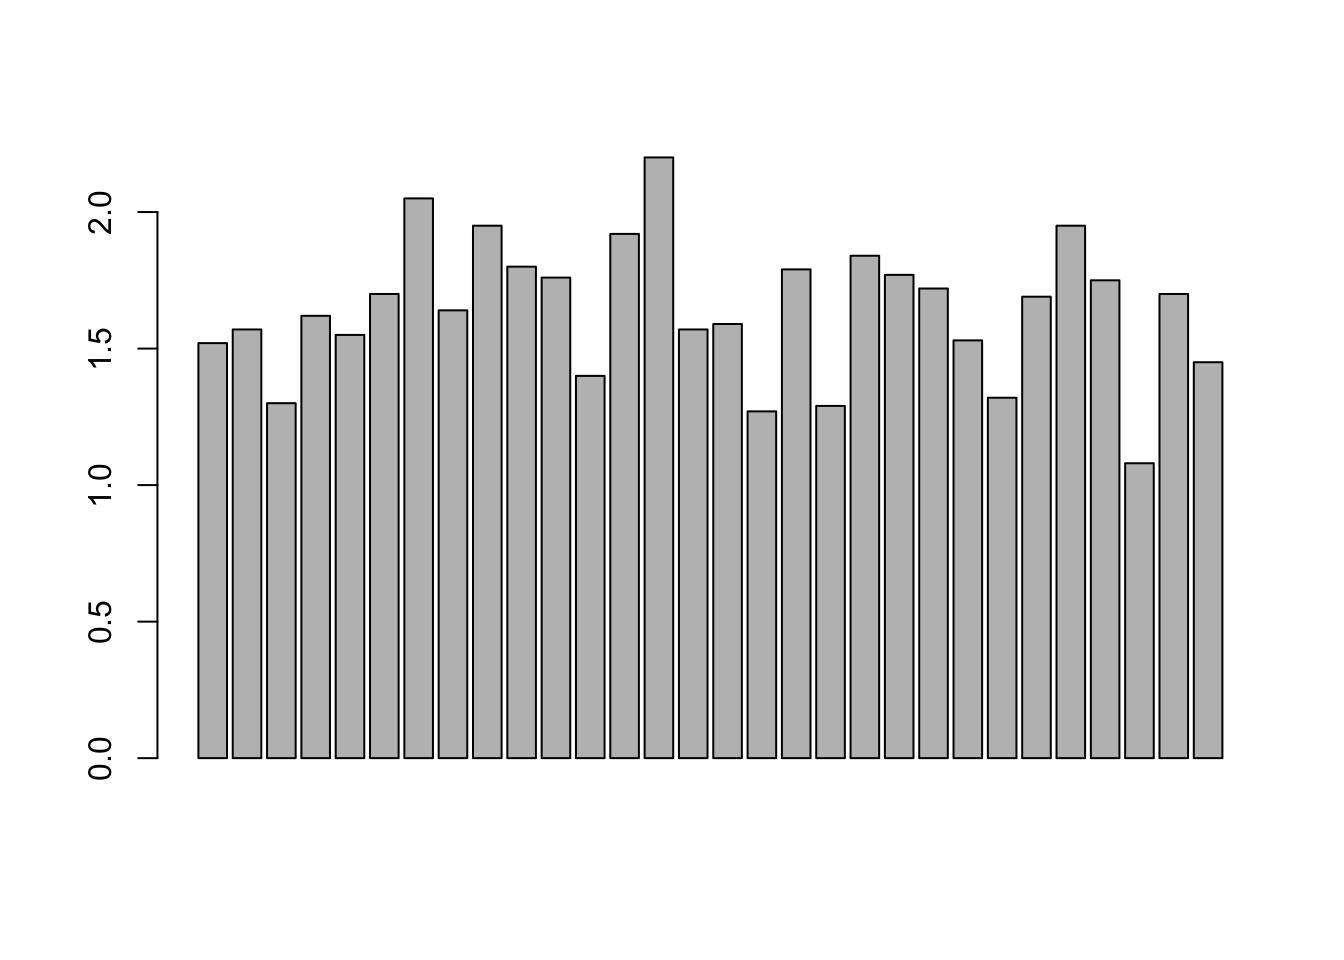
\includegraphics[width=0.7\linewidth]{bookdown-ksiazka_files/figure-latex/Barplot1-1} 

}

\caption{Barplot dla danych - Kala (2005, s. 26)}\label{fig:Barplot1}
\end{figure}

\begin{verbatim}
plot(y)  # Rys. 4.2
\end{verbatim}

\begin{figure}[H]

{\centering 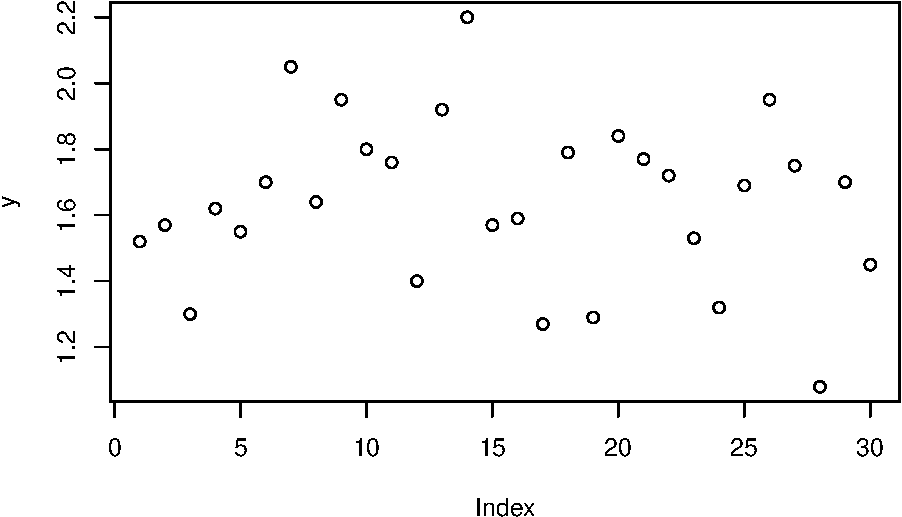
\includegraphics[width=0.7\linewidth]{bookdown-ksiazka_files/figure-latex/unnamed-chunk-48-1} 

}

\caption{Przykład użycia funkcji plot dla danych - Kala (2005, s. 26)}\label{fig:unnamed-chunk-48}
\end{figure}

\begin{verbatim}
# xlab - tytuł osi OX, ylab - tytuł osi OY, main - tytuł wykresu
plot(y,xlab="numery krzaków",ylab="wartości y w kg", main="Plony
     pomidorów") # Rys. 4.3
\end{verbatim}

\begin{figure}[H]

{\centering 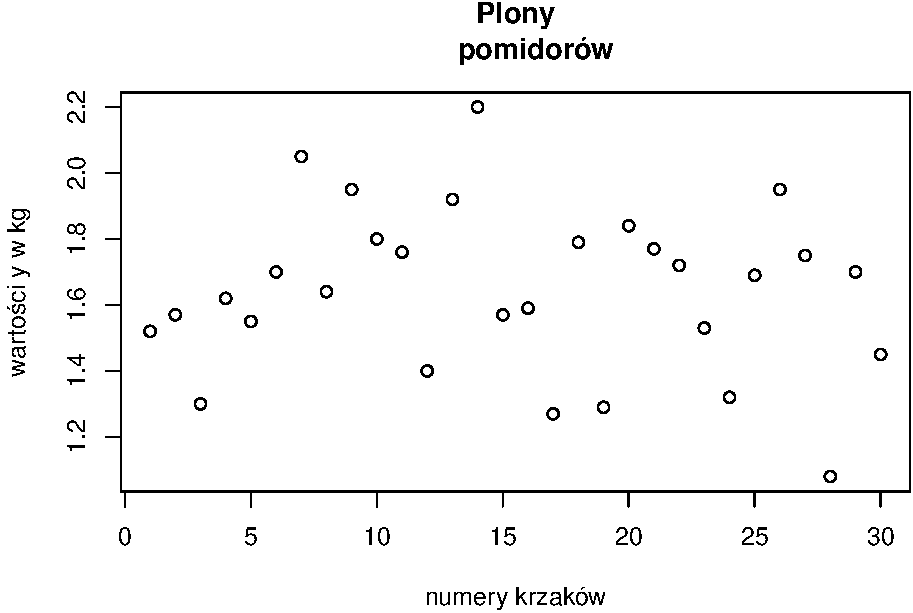
\includegraphics[width=0.7\linewidth]{bookdown-ksiazka_files/figure-latex/plott2-1} 

}

\caption{Przykład użycia funkcji plot z tytułami osi dla danych - Kala (2005, s. 26)}\label{fig:plott2}
\end{figure}

\begin{verbatim}
hist(y)  # Rys. 4.4
\end{verbatim}

\begin{figure}[H]

{\centering 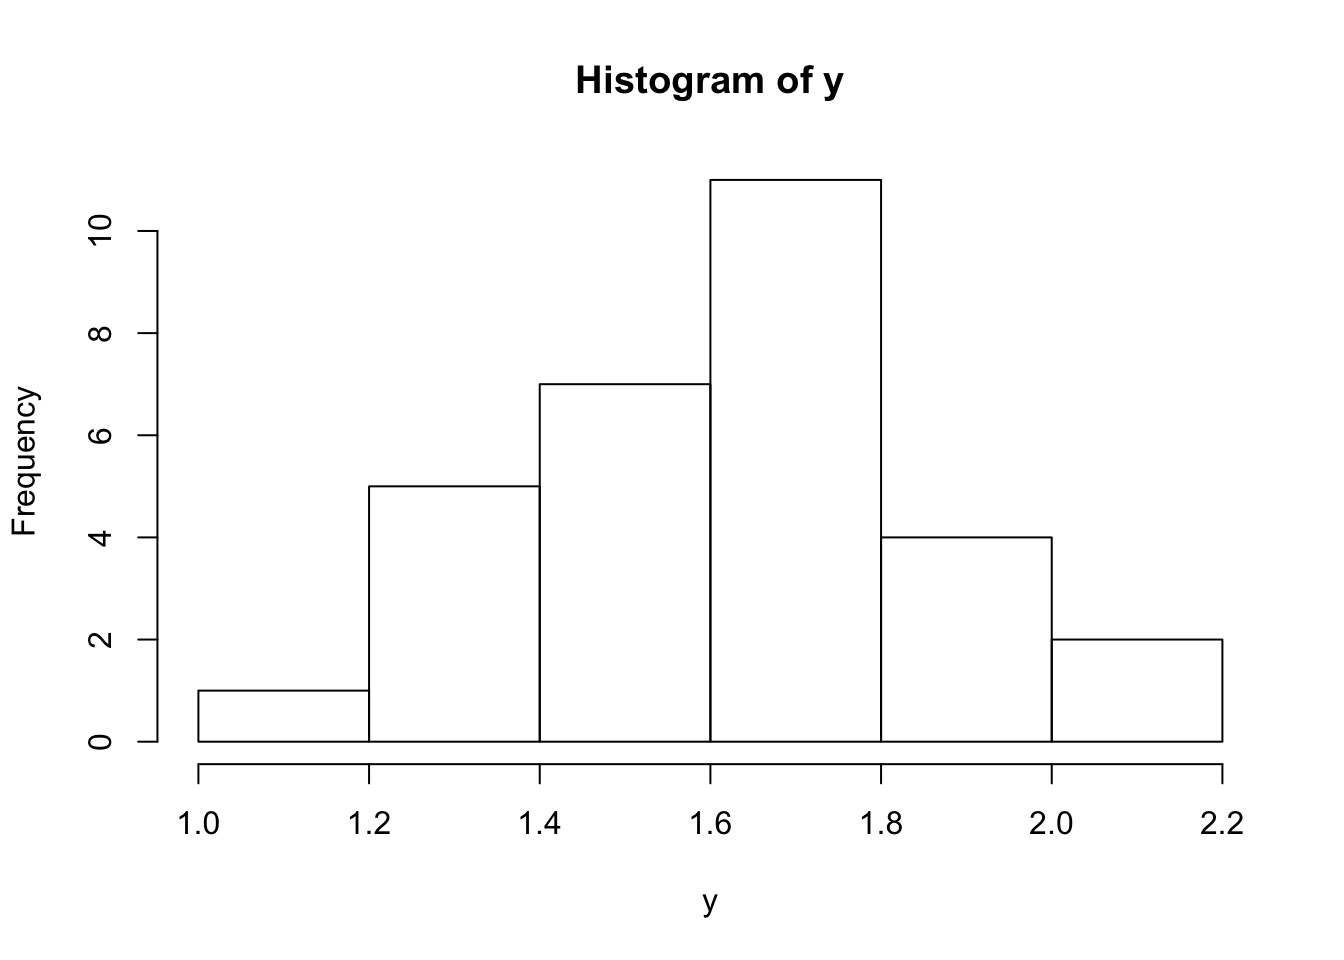
\includegraphics[width=0.7\linewidth]{bookdown-ksiazka_files/figure-latex/plott3-1} 

}

\caption{Histogram dla danych - Kala (2005, s. 26)}\label{fig:plott3}
\end{figure}

\begin{verbatim}
hist(y, main="Plonowanie pomidorów")  # Rys. 4.5
\end{verbatim}

\begin{figure}[H]

{\centering 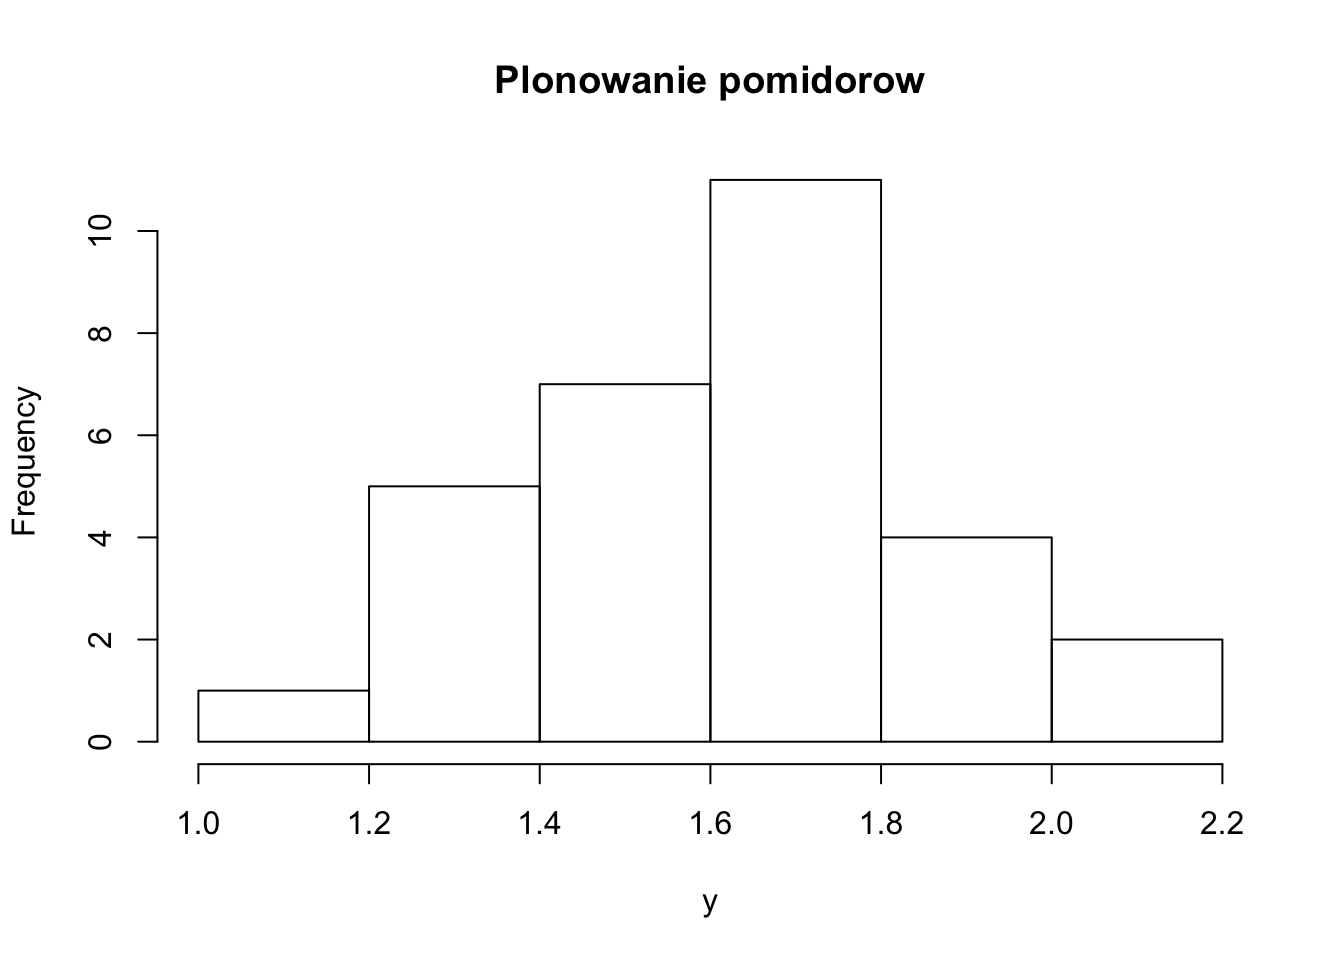
\includegraphics[width=0.7\linewidth]{bookdown-ksiazka_files/figure-latex/plott4-1} 

}

\caption{Histogram z tytułem dla danych - Kala (2005, s. 26)}\label{fig:plott4}
\end{figure}

\begin{verbatim}
# col - kolory wykresu
hist(y, col=rainbow(20), xlab="przedziały", ylab="liczebności",
     main="Plonowanie pomidorów") # Rys. 4.6
\end{verbatim}

\begin{figure}[H]

{\centering 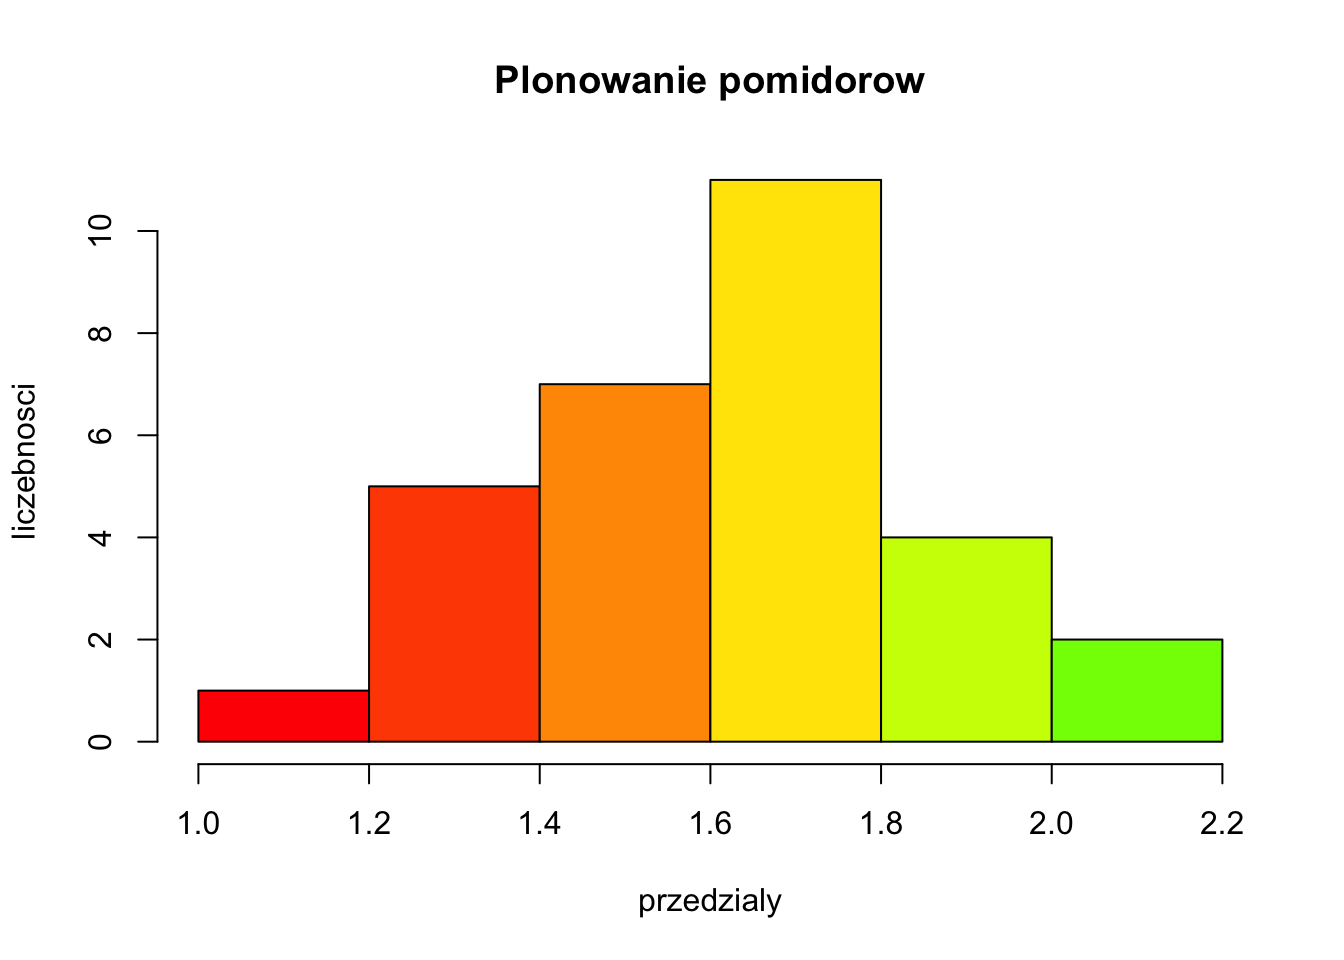
\includegraphics[width=0.7\linewidth]{bookdown-ksiazka_files/figure-latex/plott5-1} 

}

\caption{Histogram z tytułami w kolorze dla danych - Kala (2005, s. 26)}\label{fig:plott5}
\end{figure}

\begin{verbatim}
boxplot(y) # Rys. 4.7
\end{verbatim}

\begin{figure}[H]

{\centering 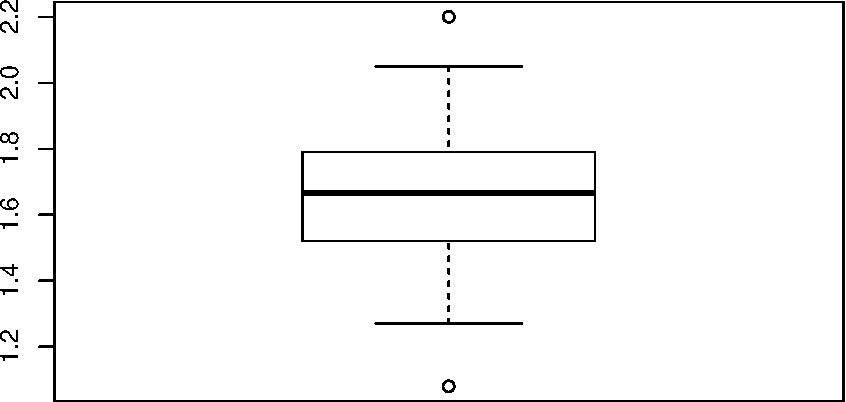
\includegraphics[width=0.7\linewidth]{bookdown-ksiazka_files/figure-latex/plott6-1} 

}

\caption{Boxplot dla danych - Kala (2005, s. 26)}\label{fig:plott6}
\end{figure}

\newpage

\textbf{Przykład 4.2} (Greń 1975, s. 161)

Dla danych z przykładu 3.1 wykonać wykres typu boxplot.

\vspace{0.8cm}

\textbf{Kod w R}

\begin{verbatim}
# Przykład 4.2 - (Greń 1975, s. 161)
# przygotowanie danych
A = c(6.7,7.3,8.0,8.0,7.9,9.2,10.1,9.2,8.3,8.4,8.0,7.9)
B = c(7.5,7.7,7.7,8.2,8.9,8.9,10.6,10.2,9.4,9.4,8.2,7.8)
C = c(5.9,6.9,7.0,7.0,9.5,9.6,9.6,10.3,8.1,8.5,8.6,8.8)
dane=data.frame(A, B, C)  # tworzenie ramki danych o nazwie "dane"
dane
boxplot(dane)   # Rys. 4.8
boxplot(dane, main="ABC")   # Rys. 4.9
\end{verbatim}

\vspace{0.8cm} \textbf{Realizacja w R}

\begin{verbatim}
> # Przykład 4.2 - (Greń 1975, s. 161)
> # przygotowanie danych
> A = c(6.7,7.3,8.0,8.0,7.9,9.2,10.1,9.2,8.3,8.4,8.0,7.9)
> B = c(7.5,7.7,7.7,8.2,8.9,8.9,10.6,10.2,9.4,9.4,8.2,7.8)
> C = c(5.9,6.9,7.0,7.0,9.5,9.6,9.6,10.3,8.1,8.5,8.6,8.8)
> dane=data.frame(A, B, C)  # tworzenie ramki danych o nazwie "dane"
> dane
\end{verbatim}

\begin{verbatim}
      A    B    C
1   6.7  7.5  5.9
2   7.3  7.7  6.9
3   8.0  7.7  7.0
4   8.0  8.2  7.0
5   7.9  8.9  9.5
6   9.2  8.9  9.6
7  10.1 10.6  9.6
8   9.2 10.2 10.3
9   8.3  9.4  8.1
10  8.4  9.4  8.5
11  8.0  8.2  8.6
12  7.9  7.8  8.8
\end{verbatim}

\begin{verbatim}
boxplot(dane) # Rys. 4.8
\end{verbatim}

\begin{figure}[H]

{\centering 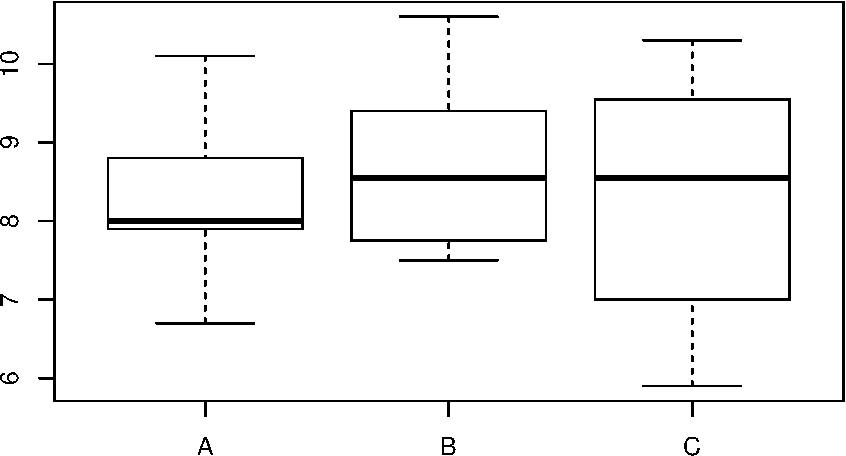
\includegraphics[width=0.57\linewidth]{bookdown-ksiazka_files/figure-latex/plott7-1} 

}

\caption{Boxplot dla danych - Greń (1975, s. 161)}\label{fig:plott7}
\end{figure}

\begin{verbatim}
boxplot(dane,main="ABC") # Rys. 4.9
\end{verbatim}

\begin{figure}[H]

{\centering 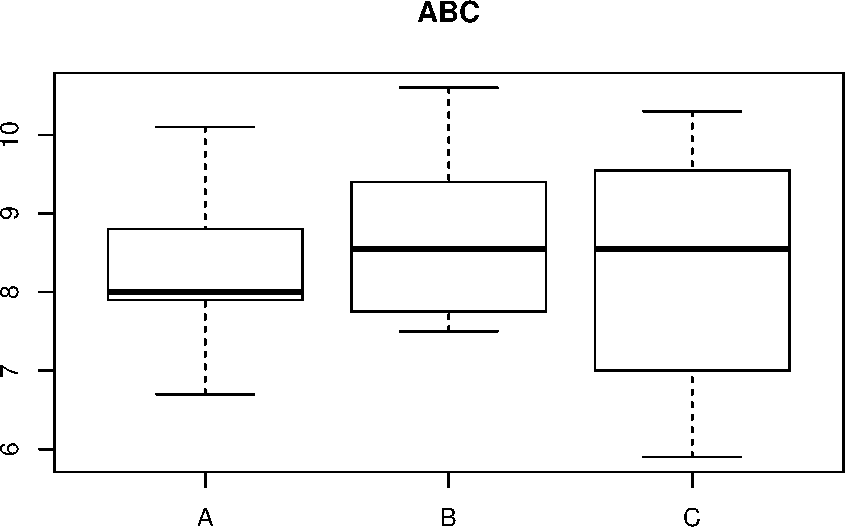
\includegraphics[width=0.57\linewidth]{bookdown-ksiazka_files/figure-latex/plott8-1} 

}

\caption{Boxplot z tytułem wykresu - Greń (1975, s. 161)}\label{fig:plott8}
\end{figure}

\section{Wykresy dla przykładowych
funkcji}\label{wykresy-dla-przykadowych-funkcji}

\vspace{0.8cm} \textbf{Przykład 4.3}

Narysować wykres funkcji \(y=x^3\) dla \(x \in \langle -10;10 \rangle\)
z osiami współrzędnych.

\vspace{0.8cm} \textbf{Kod w R}

\begin{verbatim}
# Przykład 4.3
x = -10:10  # ustalenie wartości x
x # wyświetlenie zawartości x
y=x^3  # obliczenie wartości y
plot(x, y)  # Rys. 4.10
# pch - określenie znaków (symboli) na wykresie
plot(x, y, pch = 1:20) # zmiana wartości argumentu 'pch'  -  Rys. 4.11
lines(x,y)  # dodanie linii łączących x i y  - Rys. 4.12
abline(h=0)  # dodanie linii poziomej y=0, czyli osi OX
abline(v=0, col="red") # dodanie czerwonej linii pionowej x=0 (oś OY)  - Rys. 4.13
\end{verbatim}

\vspace{0.8cm} \textbf{Realizacja w R}

\begin{verbatim}
> # Przykład 4.3
> x = -10:10  # ustalenie wartości x
> x # wyświetlenie zawartości x
\end{verbatim}

\begin{verbatim}
 [1] -10  -9  -8  -7  -6  -5  -4  -3  -2  -1   0   1   2   3   4   5   6
[18]   7   8   9  10
\end{verbatim}

\begin{verbatim}
> y=x^3  # obliczenie wartości y
\end{verbatim}

\begin{verbatim}
plot(x, y)  # Rys. 4.10
\end{verbatim}

\begin{figure}[H]

{\centering 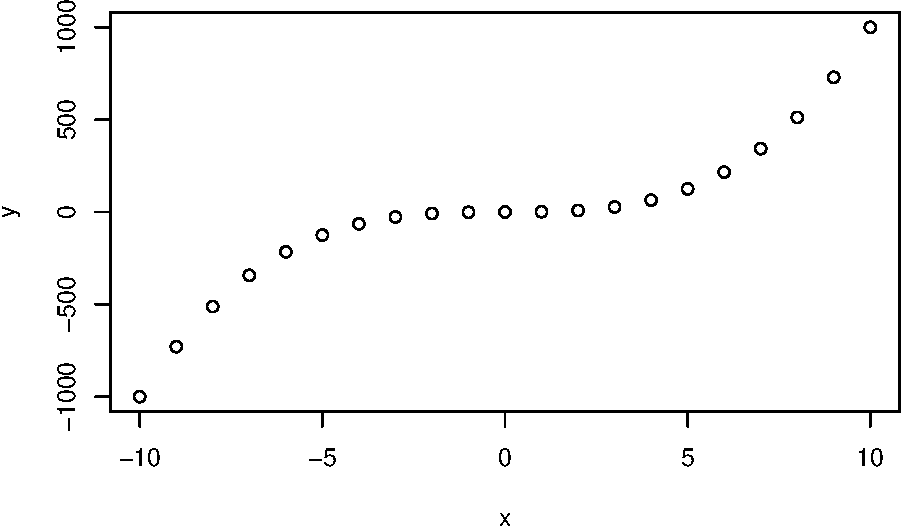
\includegraphics[width=0.7\linewidth]{bookdown-ksiazka_files/figure-latex/plott9-1} 

}

\caption{Wykres funkcji $y=x^3$}\label{fig:plott9}
\end{figure}

\begin{verbatim}
# pch - określenie znaków (symboli) na wykresie
plot(x, y, pch = 1:20) # zmiana wartości argumentu 'pch' -  Rys. 4.11
\end{verbatim}

\begin{figure}[H]

{\centering 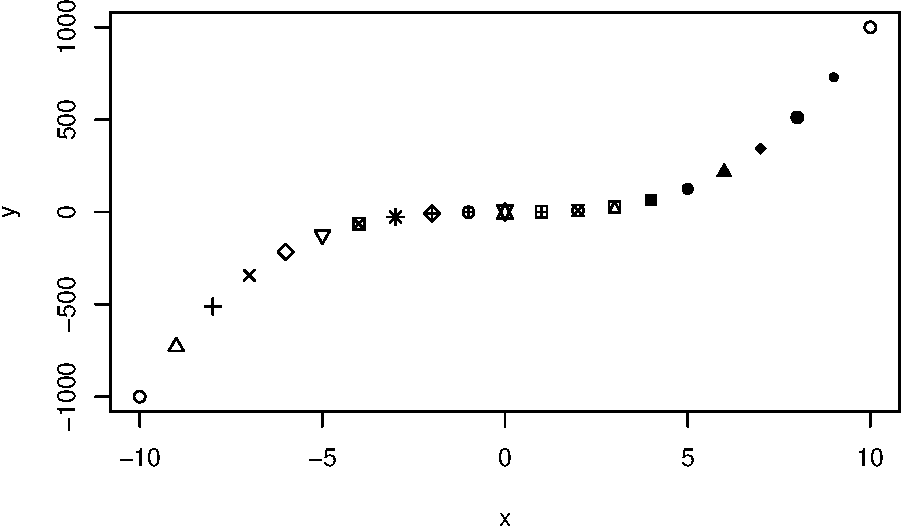
\includegraphics[width=0.7\linewidth]{bookdown-ksiazka_files/figure-latex/plott9a-1} 

}

\caption{Wykres funkcji $y=x^3$ ze zmianą wartości pch}\label{fig:plott9a}
\end{figure}

\newpage

\begin{verbatim}
lines(x,y)  # dodanie linii łączących x i y -  Rys. 4.12
\end{verbatim}

\begin{figure}[H]

{\centering 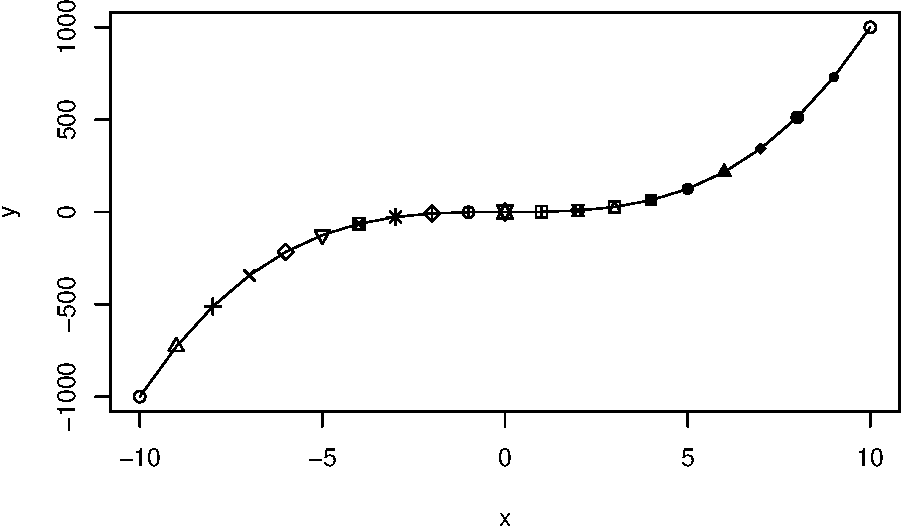
\includegraphics[width=0.7\linewidth]{bookdown-ksiazka_files/figure-latex/unnamed-chunk-54-1} 

}

\caption{Wykres funkcji $y=x^3$ z liniami łączącymi}\label{fig:unnamed-chunk-54}
\end{figure}

\begin{verbatim}
abline(h=0)  # dodanie linii poziomej y=0, czyli osi OX
abline(v=0, col="red") # dodanie czerwonej linii pionowej x=0 (oś OY)  - Rys. 4.13
\end{verbatim}

\begin{figure}[H]

{\centering 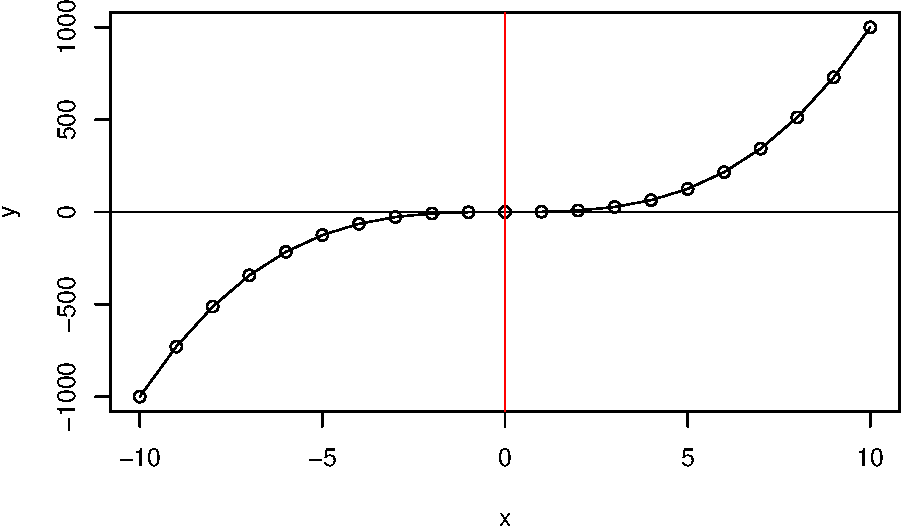
\includegraphics[width=0.7\linewidth]{bookdown-ksiazka_files/figure-latex/unnamed-chunk-56-1} 

}

\caption{Wykres funkcji $y=x^3$ z osiami OX i OY}\label{fig:unnamed-chunk-56}
\end{figure}

\textbf{Przykład 4.4}

Narysować w jednym „oknie'' wykresy funkcji \(y=sin(x)\) oraz
\(y=cos(x)\) dla \(x \in \langle -3 \pi;3 \pi \rangle\).

\vspace{0.8cm} \textbf{Kod w R}

\begin{verbatim}
# Przykład 4.4
# ustalamy wartości x
x = seq(-3*pi, 3*pi, by=0.3)
# rysujemy funkcję sin(x) - type='l' oznacza linię
plot(x, sin(x), type="l", main="Wykres funkcji sin(x) i cos(x)", col="red")  # Rys. 4.14
# dorysowujemy funkcję cos(x) i nadajemy tytuł osi OY
lines(x, cos(x),  col="blue", type="l", ylab='wartości funkcji')  # Rys. 4.15
\end{verbatim}

\vspace{0.8cm} \textbf{Realizacja w R}

\begin{verbatim}
> # Przykład 4.4
> # ustalamy wartości x
> x = seq(-3*pi, 3*pi, by=0.3)
\end{verbatim}

\begin{verbatim}
# rysujemy funkcję sin(x) - type='l'
# oznacza linię
plot(x, sin(x), type = "l", main = "Wykres funkcji sin(x) i cos(x)", 
    col = "red")  # Rys. 4.14
\end{verbatim}

\begin{figure}[H]

{\centering 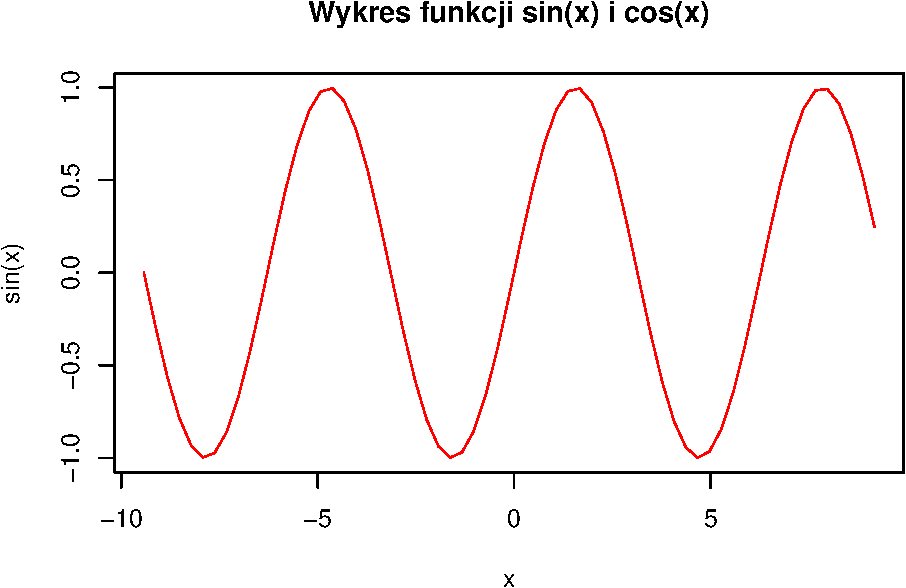
\includegraphics[width=0.7\linewidth]{bookdown-ksiazka_files/figure-latex/unnamed-chunk-59-1} 

}

\caption{Wykres funkcji $y=sin(x)$}\label{fig:unnamed-chunk-59}
\end{figure}

\begin{verbatim}
# dorysowujemy funkcję cos(x) i nadajemy tytuł osi OY
lines(x, cos(x),  col="blue", type="l", ylab='wartości funkcji')  # Rys. 4.15
\end{verbatim}

\begin{figure}[H]

{\centering 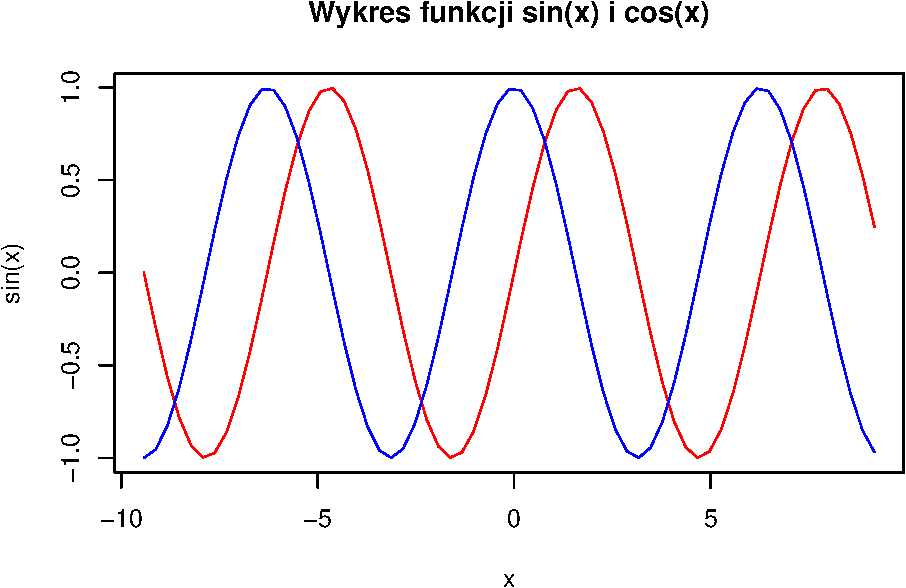
\includegraphics[width=0.7\linewidth]{bookdown-ksiazka_files/figure-latex/lines-1} 

}

\caption{Wykresy funkcji $y=sin(x)$ oraz $y=cos(x)$ przy pomocy funkcji plot i lines}\label{fig:lines}
\end{figure}

\vspace{0.8cm} \textbf{Przykład 4.5}

Narysować w jednym `oknie' wykresy funkcji \(y=sin(x)\) oraz
\(y=cos(x)\) dla \(x \in \langle -3 \pi;3 \pi \rangle\) przy pomocy
funkcji `curve'.

\vspace{0.8cm} \textbf{Kod w R}

\begin{verbatim}
# Przykład 4.5 - funkcja 'curve' Rys. 4.16
curve(sin, from = -3 * pi, to = 3 * pi, type = "l", col = "red", xlab = "argumenty funkcji", 
    ylab = "wartości funkcji")
curve(cos, from = -3 * pi, to = 3 * pi, type = "b", col = "blue", add = T)
title(main = "Wykres funkcji y=sin(x) i y=cos(x)")
\end{verbatim}

\newpage

\textbf{Realizacja w R}

\begin{verbatim}
# Przykład 4.5 - funkcja 'curve' Rys. 4.16
curve(sin, from = -3 * pi, to = 3 * pi, type = "l", col = "red", xlab = "argumenty funkcji", 
    ylab = "wartości funkcji")
curve(cos, from = -3 * pi, to = 3 * pi, type = "b", col = "blue", add = T)
title(main = "Wykres funkcji y=sin(x) i y=cos(x)")
\end{verbatim}

\begin{figure}[H]

{\centering 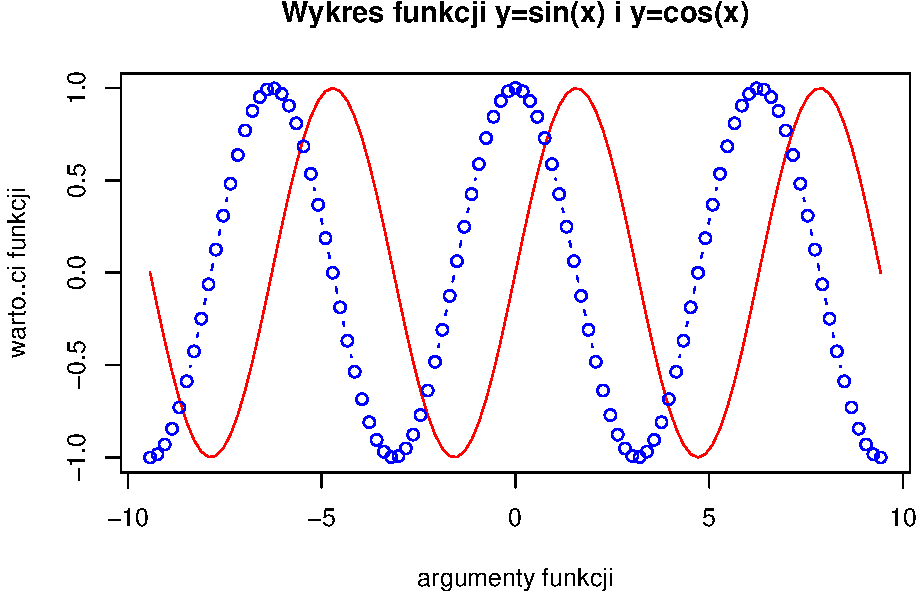
\includegraphics[width=0.7\linewidth]{bookdown-ksiazka_files/figure-latex/unnamed-chunk-62-1} 

}

\caption{Wykresy funkcji $y=sin(x)$ oraz $y=cos(x)$ przy pomocy funkcji curve}\label{fig:unnamed-chunk-62}
\end{figure}

\section{Zadania do wykonania}\label{zadania-do-wykonania-3}

Zad. 1

Wczytaj dane ``Studenci.xlsx'' i wykonaj wykres funkcją \texttt{plot}
typu punktowego, gdzie na osi X znajdować się będzie wiek studentów, a
na osi Y wysokość stypendium. Zaznacz kolorem czerwonym kobiety, a
niebieskim mężczyzn.

\newpage

Zad. 2

Na jednym wykresie narysuj w przedziale \([-5, 5]\) następujące funkcje:
\(y = x^2\); \(y = (x-2)^2\); \(y = (x-2)^2+3\); \(y = x^2+3\);
\(y = (x+1)^2-2\). Dodaj linie \(x = 0\) w kolorze czarnym. Każda
funkcja niech będzie narysowana innym kolorem. Nadaj tytuł: ``Wykresy
funkcji przesuniętych''.

\vspace{0.8cm} Zad. 3

Narysuj histogram dla wysokości stypendium dla danych z pliku
``Studenci.xlsx''.

\chapter{Testowanie}\label{testowanie}

\section{Wprowadzenie}\label{wprowadzenie}

Niech dane będą 2 populacje, dla których chcemy zweryfikować
interesujące nas przypuszczenie. Na przykład, dane jest 200 ha pole z
pszenżytem odmiany A oraz 150 ha pole z pszenżytem odmiany B. Chcemy
porównać ciężar nasion w kłosie dla obu odmian. Oczywiście, najlepszym
sposobem postępowania jest zważenie nasion wszystkich kłosów z obu pól.
Jak wiadomo, taka czynność nie jest wykonywana. Powinniśmy losowo wybrać
kilkanaście lub kilkadziesiąt kłosów z pierwszego pola (próba A) i
drugiego pola (próba B). Tak więc mamy populacje oraz mamy próby, gdzie
najczęściej stosowane oznaczenia wybranych parametrów przedstawia
Tablica \ref{testowanie}.

\begin{table}[H]
\centering
\caption{Podstawowe parametry dla populacji oraz próby}
\label{testowanie}
\begin{tabular}{cc}
\hline
populacja & próba                                     \\ \hline
$\mu$ – średnia cechy w populacji                & $\bar{x}$ – średnia cechy w próbie               \\
$\sigma^2$ – wariancja cechy w populacji             & $s^2$ – wariancja cechy w próbie             \\
$\sigma$ – odchylenie standardowe cechy w populacji & $s$ – odchylenie standardowe cechy w próbie \\ \hline
\end{tabular}
\end{table}

Testowanie jest to weryfikacja przypuszczeń. W opracowaniu tym
rozpatrujemy testy parametryczne, czyli testy dotyczące parametrów
populacji (np. średnia, wariancja). Przypuszczenia określone są przy
pomocy dwóch hipotez: hipotezy zerowej \(H_0\) oraz hipotezy
alternatywnej \(H_1\). Po wybraniu właściwej statystyki, wyliczamy
wartość tej statystyki dla wylosowanych prób oraz tzw. \(p\)-wartość
(\(p\)-value) i podejmujemy decyzję: albo odrzucamy hipotezę zerową i
przyjmujemy hipotezę alternatywną, albo stwierdzamy brak podstaw do
odrzucenia hipotezy zerowej (w praktyce często przyjmuje się hipotezę
zerową). Porównując rzeczywistość z naszą decyzją możemy mieć sytuacje
przedstawione w Tablicy \ref{decyzje}. Prawdopodobieństwo odrzucenia
hipotezy prawdziwej jest błędem pierwszego rodzaju oznaczanym przez
\(\alpha\) oraz nazywanym poziomem istotności. Natomiast
prawdopodobieństwo przyjęcia hipotezy nieprawdziwej jest błędem drugiego
rodzaju oznaczanym przez \(\beta\).

\begin{table}[H]
\centering
\caption{Możliwe decyzji podczas testowania}
\label{decyzje}
\begin{tabular}{cc|c|c|}
\cline{3-4}
\multicolumn{2}{c}{\multirow{2}{*}{}}                                       & \multicolumn{2}{|c|}{Decyzja} \\ \cline{3-4} 
\multicolumn{2}{c|}{}                                                        & $H_0$ nie odrzucamy  & $H_0$ odrzucamy \\ \hline
\multicolumn{1}{|c|}{\multirow{2}{*}{Rzeczywistość}} & $H_0$ jest prawdziwa          & OK             & $\alpha$          \\ \cline{2-4} 
\multicolumn{1}{|c|}{}                               & $H_0$ nie jest prawdziwa & $\beta$              & OK          \\ \hline
\end{tabular}
\end{table}

Reguły postępowania podczas testowania hipotez:

\begin{enumerate}
\def\labelenumi{\arabic{enumi}.}
\item
  Mamy dane populacje w ramach których chcemy wykonać testowanie.
\item
  Formułujemy problem badawczy.
\item
  Ustalamy poziom istotności \(\alpha\), np. w tym manuskrypcie
  \(\alpha\) = 0.05.
\item
  Formułujemy hipotezę zerową \(H_0\) oraz hipotezę alternatywną
  \(H_1\).
\item
  Losowo wybieramy próby.
\item
  Ustalamy właściwą statystykę (odpowiedni test) do weryfikacji hipotez.
\item
  Obliczamy wartości wybranej statystki, m.in. \(p\)-wartość.
\item
  Podejmujemy decyzje:

  8.1. jeśli \(p\)-wartość \textless{}0.05 (poziom istotności), to
  odrzucamy hipotezę zerową i przyjmujemy hipotezę alternatywną,

  8.2. jeśli \(p\)-wartość \(\geq\) 0.05, to nie mamy podstaw do
  odrzucenia \(H_0\), co w praktyce często oznacza przyjęcie hipotezy
  zerowej.
\item
  Dokonujemy interpretacji problemu badawczego.
\end{enumerate}

\begin{table}[H]
\centering
\caption{Wybrane testy statystyczne dla wartości średnich}
\label{testy}
\begin{tabular}{cc|c |c|}
\cline{3-4}
\multicolumn{2}{c|}{}                                                                                                               & Dane z rozkładu normalnego                                                       & \begin{tabular}[c]{@{}c@{}}Dane nie są z rozkładu \\ normalnego\end{tabular}    \\ \hline
\multicolumn{1}{|c|}{}                                                                                      & 2 grupy              & \begin{tabular}[c]{@{}c@{}}Test t dla grup niezależnych\\ (t.test)*\end{tabular} & \begin{tabular}[c]{@{}c@{}}Test Wilcoxona\\ (Wilcox.test)\end{tabular}          \\ \cline{2-4} 
\multicolumn{1}{|c|}{\multirow{-2}{*}{Próby niezależne}}                                                    & \textgreater 2 grupy & \begin{tabular}[c]{@{}c@{}}ANOVA\\ (aov)\end{tabular}                            & \begin{tabular}[c]{@{}c@{}}Test Kruskala-Wallisa\\ (kruskal.test)\end{tabular}  \\ \hline
\multicolumn{1}{|c|}{}                                                                                      & 2 grupy              & \begin{tabular}[c]{@{}c@{}}Test t związany\\ (t.test)\end{tabular}  & \begin{tabular}[c]{@{}c@{}}Test Wilcoxona związany\\ (wilcox.test)\end{tabular} \\  \cline{2-4} 
\multicolumn{1}{|c|}{\multirow{-2}{*}{\begin{tabular}[c]{@{}c@{}}Próby zależne\\  (związane)\end{tabular}}} & \textgreater 2grupy  & \begin{tabular}[c]{@{}c@{}}ANOVA\\ (aov)\end{tabular}                            & \begin{tabular}[c]{@{}c@{}}Test Friedmana\\ (friedman.test)\end{tabular}        \\ \hline
\end{tabular}
\end{table}

\(\ast\) w nawiasach podane są nazwy funkcji w R.

Tablica \ref{testy} wskazuje, że wybór testu zależy od trzech
charakterystyk:

\begin{enumerate}
\def\labelenumi{\arabic{enumi}.}
\tightlist
\item
  Czy dane podlegają rozkładowi normalnemu, czy nie podlegają,
\item
  Czy próby są niezależne, czy są zależne,
\item
  Czy rozpatrujemy dwie próby (grupy), czy więcej niż dwie.
\end{enumerate}

\vspace{0.8cm} \textbf{Uwaga}

\begin{enumerate}
\def\labelenumi{\arabic{enumi})}
\item
  Sprawdzenie normalności rozkładu w R można przeprowadzić stosując
  funkcję \texttt{shapiro.test} - test Shapiro--Wilka.
\item
  Przed zastosowaniem testu \(t\) (\texttt{t.test}) należy sprawdzić,
  czy założenie o równości wariancji jest spełnione. W R można to
  wykonać np. przy pomocy funkcji \texttt{var.test}.
\end{enumerate}

\section{Testy dwóch wartości średnich z rozkładów
normalnych}\label{testy-dwoch-wartosci-srednich-z-rozkadow-normalnych}

\textbf{Założenie}

Mamy dwie próby odpowiednio o liczebności \(n_1\) z rozkładu
\(N(\mu_1, \sigma_1^2)\) oraz o liczebności \(n_2\) z rozkładu
\(N(\mu_2, \sigma_2^2)\).

Możemy rozpatrywać hipotezę dwustronną, hipotezę lewostronną lub
hipotezę prawostronną.

\vspace{0.8cm} \textbf{Hipotezy}

\begin{enumerate}
\def\labelenumi{\alph{enumi})}
\tightlist
\item
  hipoteza dwustronna (test obustronny) \vspace{-0.6cm}

  \begin{align}
      H_0: \mu_1 = \mu_2  \\
      H_1: \mu_1 \neq \mu_2 \nonumber
  \end{align}
\item
  hipoteza lewostronna (test lewostronny) \vspace{-0.6cm}

  \begin{align}
      H_0: \mu_1 = \mu_2 \\
      H_1: \mu_1 < \mu_2 \nonumber
  \end{align}
\item
  hipoteza prawostronna (test prawostronny) \vspace{-0.6cm}

  \begin{align}
      H_0: \mu_1 = \mu_2 \\
      H_1: \mu_1 > \mu_2 \nonumber
  \end{align}
\end{enumerate}

Rozpatrujemy dwie sytuacje: próby są niezależne lub próby są zależne
(związane, sprzężone).

\subsection{Próby niezależne}\label{proby-niezalezne}

\vspace{0.8cm} \textbf{Przykład 5.1} (Elandt 1964, s. 102)

Dany jest ciężar w gramach 1000 nasion dla dwóch rodów seradeli:

\begin{table}[H]
\centering
\caption{Dane - Elandt (1964, s. 102)}
\label{saradele}
\begin{tabular}{cc}
\hline
Ród A &  Ród B \\ \hline
3.8   &  3.7          \\
3.7   &  4.6          \\
2.9   &  5.4          \\
3.5   &  6.2          \\
2.6   &  4.2          \\
3.3   &  3.5          \\
      & 5.3          \\
      & 5.5     \\ \hline     
\end{tabular}
\end{table}

Zweryfikować przypuszczenie, że średnie ciężary tych rodów różnią się
istotnie.

\vspace{0.8cm} \textbf{Rozwiązanie}

Niech \(\mu_1\) oznacza średni ciężar 1000 nasion rodu A, natomiast
\(\mu_2\) oznacza średni ciężar 1000 nasion rodu B. Rozpatrujemy
hipotezę obustronną postaci (5.1):

\vspace{-0.6cm}

\begin{align*}
        H_0: \mu_1 = \mu_2 \\
        H_1: \mu_1 \neq \mu_2
\end{align*}

\vspace{0.8cm} \textbf{Kod w R}

\begin{verbatim}
# Przykład 5.1 (Elandt 1964, s. 102)
# tworzenie danych
rodA=c(3.8, 3.7, 2.9, 3.5, 2.6, 3.3)
rodB=c(3.7, 4.6, 5.4, 6.2, 4.2, 3.5, 5.3, 5.5)
# Boxplot - prezentacja graficzna danych
boxplot(rodA, rodB, names=c("Ród A","Ród B"), main="seradela")
\end{verbatim}

\vspace{0.8cm} \textbf{Realizacja w R}

\begin{verbatim}
> # Przykład 5.1 (Elandt 1964, s. 102)
> # tworzenie danych
> rodA=c(3.8, 3.7, 2.9, 3.5, 2.6, 3.3)
> rodB=c(3.7, 4.6, 5.4, 6.2, 4.2, 3.5, 5.3, 5.5)
> # Boxplot - prezentacja graficzna danych
> boxplot(rodA, rodB, names=c("Ród A","Ród B"), main="seradela")
\end{verbatim}

\begin{figure}[H]

{\centering 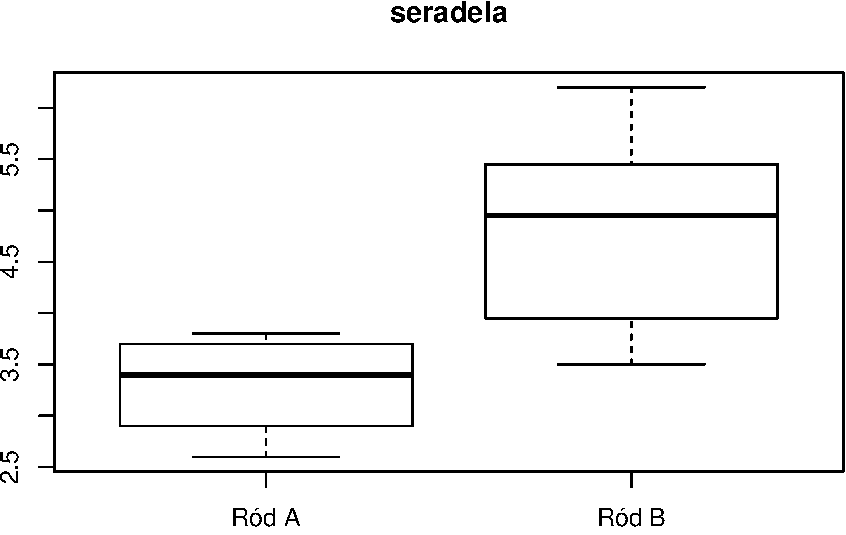
\includegraphics[width=0.7\linewidth]{bookdown-ksiazka_files/figure-latex/unnamed-chunk-64-1} 

}

\caption{Boxplot dla danych - Elandt (1964, s. 102)}\label{fig:unnamed-chunk-64}
\end{figure}

Sprawdzamy założenie o normalności rozkładów dla rodu A oraz rodu B

\hspace*{5cm} \(H_0\): rozkład normalny jest spełniony

\hspace*{5cm} \(H_1\): rozkład normalny nie jest spełniony

\vspace{0.8cm} \textbf{Kod w R}

\begin{verbatim}
# sprawdzenie założeń o normalności rozkładów dla rodu A oraz rodu B
shapiro.test(rodA)
shapiro.test(rodB)
\end{verbatim}

\vspace{0.8cm} \textbf{Realizacja w R}

\begin{verbatim}
> # sprawdzenie założeń o normalności rozkładów dla rodu A oraz rodu B
> shapiro.test(rodA)
\end{verbatim}

\begin{verbatim}

    Shapiro-Wilk normality test

data:  rodA
W = 0.93433, p-value = 0.6139
\end{verbatim}

\begin{verbatim}
> shapiro.test(rodB)
\end{verbatim}

\begin{verbatim}

    Shapiro-Wilk normality test

data:  rodB
W = 0.94586, p-value = 0.6694
\end{verbatim}

\vspace{0.8cm} \textbf{Interpretacja}

Po zastosowaniu testu Shapiro--Wilka dla obu rodów otrzymane
\(p\)-wartości są większe od 0.05. Stwierdzamy, że założenia o
normalności rozkładów są spełnione. Kolejnym krokiem jest sprawdzenie
równości wariancji obu rodów.

\vspace{0.8cm} \textbf{Kod w R}

\begin{verbatim}
var.test(rodA,rodB)
\end{verbatim}

\vspace{0.8cm} \textbf{Realizacja w R}

\begin{verbatim}
> var.test(rodA,rodB)
\end{verbatim}

\begin{verbatim}

    F test to compare two variances

data:  rodA and rodB
F = 0.24214, num df = 5, denom df = 7, p-value = 0.1377
alternative hypothesis: true ratio of variances is not equal to 1
95 percent confidence interval:
 0.0458141 1.6593925
sample estimates:
ratio of variances 
         0.2421384 
\end{verbatim}

\vspace{0.8cm} \textbf{Interpretacja}

Testowanie równości wariancji pokazuje, że otrzymana \(p\)-wartość =
0.1377 \textgreater{} 0.05, zatem nie ma podstaw do odrzucenia hipotezy
mówiącej o równości wariancji obu rodów. W tym przypadku wykonując w
kolejnym kroku testowanie hipotez (5.1) wykorzystujemy dwustronny test
\(t\), przy użyciu funkcji \texttt{t.test} z zastosowaniem dodatkowo
argumentu \texttt{var.equal=TRUE} oznaczającego równość wariancji. W
przeciwnym przypadku ustawiana jest domyślnie wartość
\texttt{var.equal=FALSE} (co oznacza, że wariancje nie są równe) oraz
stosowane jest przybliżenie Welcha.

\vspace{0.8cm} \textbf{Kod w R}

\begin{verbatim}
# obustronny test t
t.test(rodA, rodB, var.equal = TRUE)
\end{verbatim}

\vspace{0.8cm} \textbf{Realizacja w R}

\begin{verbatim}
> # obustronny test t
> t.test(rodA, rodB, var.equal = TRUE)
\end{verbatim}

\begin{verbatim}

    Two Sample t-test

data:  rodA and rodB
t = -3.5226, df = 12, p-value = 0.004203
alternative hypothesis: true difference in means is not equal to 0
95 percent confidence interval:
 -2.4277738 -0.5722262
sample estimates:
mean of x mean of y 
      3.3       4.8 
\end{verbatim}

\vspace{0.8cm} \textbf{Interpretacja}

Ponieważ \(p\)-wartość = 0.004203 \textless{} 0.05, więc stwierdzamy, że
ciężar 1000 nasion seradeli rodu A różni się od rodu B. Ponadto,
analizując boxplot (Rys. 5.1) można przypuszczać, że ciężar 1000 nasion
dla rodu A seradeli jest mniejszy niż ciężar 1000 nasion dla rodu B
seradeli. Wobec tego, zastosujemy lewostronny test \(t\) postaci (5.2),
czyli: \vspace{-0.6cm}

\begin{align*}
        H_0: \mu_1 = \mu_2 \\
        H_1: \mu_1 < \mu_2
\end{align*}

\vspace{0.8cm} \textbf{Kod w R}

\begin{verbatim}
# lewostronny test t
t.test(rodA, rodB, alternative="less", var.equal = TRUE)
\end{verbatim}

\vspace{0.8cm} \textbf{Realizacja w R}

\begin{verbatim}
> # lewostronny test t
> t.test(rodA, rodB, alternative="less", var.equal = TRUE)
\end{verbatim}

\begin{verbatim}

    Two Sample t-test

data:  rodA and rodB
t = -3.5226, df = 12, p-value = 0.002101
alternative hypothesis: true difference in means is less than 0
95 percent confidence interval:
       -Inf -0.7410731
sample estimates:
mean of x mean of y 
      3.3       4.8 
\end{verbatim}

\vspace{0.8cm} \textbf{Interpretacja}

Ponieważ \(p\)-wartość = 0.002101 \textless{} 0.05, więc stwierdzamy, że
ciężar 1000 nasion rodu A seradeli jest mniejszy niż rodu B.

\subsection{Próby zależne}\label{proby-zalezne}

\vspace{0.8cm} \textbf{Przykład 5.2} (Elandt 1964, s. 109)

Oznaczono procent tłuszczu w 18 próbkach mleka za pomocą dwóch metod:
metody Gerbera (metoda G) i metody Burata (metoda B) - patrz Tablica
\ref{mleko}.

\begin{table}[!ht]
\centering
\caption{Dane - Elandt (1964, s. 109)}
\label{mleko}
\begin{tabular}{ccc|ccc}
\hline
Lp. & Metoda G & Metoda B & Lp. & Metoda G & Metoda B \\ \hline
1   & 2.73     & 2.88     & 10  & 3.07     & 3.23     \\
2   & 2.84     & 2.93     & 11  & 2.66     & 2.81     \\
3   & 3.18     & 3.38     & 12  & 2.78     & 2.94     \\
4   & 2.79     & 2.99     & 13  & 3.62     & 3.59     \\
5   & 3.05     & 3.30     & 14  & 3.31     & 3.41     \\
6   & 3.03     & 3.19     & 15  & 2.71     & 2.88     \\
7   & 3.10     & 3.34     & 16  & 2.80     & 2.99     \\
8   & 2.88     & 3.08     & 17  & 2.95     & 3.16     \\
9   & 3.00     & 3.20     & 18  & 3.52     & 3.66    \\ \hline
\end{tabular}
\end{table}

Czy metody te dają takie same wyniki?

\textbf{Kod w R}

\begin{verbatim}
# Przykład 5.2 (Elandt 1964, s. 109)
rm(list=ls()) # usuwanie wszystkich zmiennych z przestrzeni roboczej
# tworzenie danych
metodaG=c(2.73, 2.84, 3.18, 2.79, 3.05, 3.03, 3.10, 2.88, 3.00, 3.07,
          2.66, 2.78, 3.62, 3.31, 2.71, 2.80, 2.95, 3.52)
metodaB=c(2.88, 2.93, 3.38, 2.99, 3.30, 3.19, 3.34, 3.08, 3.20, 3.23,
          2.81, 2.94, 3.59, 3.41, 2.88, 2.99, 3.16, 3.66)
dane=data.frame(metodaG,metodaB)
# prezentacja graficzna danych - boxplot
boxplot(metodaG, metodaB, main="Procent tłuszczu")
# Sprawdzamy założenia o normalności rozkładów
shapiro.test(metodaG)
shapiro.test(metodaB)
\end{verbatim}

\vspace{0.8cm} \textbf{Realizacja w R}

\begin{verbatim}
> # Przykład 5.2 (Elandt 1964, s. 109)
> rm(list=ls()) # usuwanie wszystkich zmiennych z przestrzeni roboczej
> # tworzenie danych
> metodaG=c(2.73, 2.84, 3.18, 2.79, 3.05, 3.03, 3.10, 2.88, 3.00, 3.07,
+           2.66, 2.78, 3.62, 3.31, 2.71, 2.80, 2.95, 3.52)
> metodaB=c(2.88, 2.93, 3.38, 2.99, 3.30, 3.19, 3.34, 3.08, 3.20, 3.23,
+           2.81, 2.94, 3.59, 3.41, 2.88, 2.99, 3.16, 3.66)
> dane=data.frame(metodaG,metodaB)
> # prezentacja graficzna danych - boxplot
> boxplot(dane, main="Procent tłuszczu")
\end{verbatim}

\begin{figure}[H]

{\centering 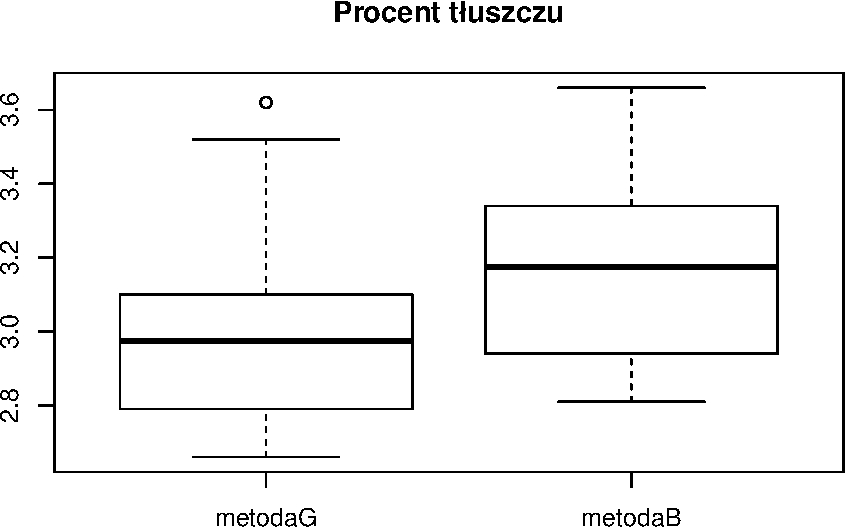
\includegraphics[width=0.7\linewidth]{bookdown-ksiazka_files/figure-latex/unnamed-chunk-74-1} 

}

\caption{Boxplot dla danych - Elandt (1964, s. 109)}\label{fig:unnamed-chunk-74}
\end{figure}

\begin{verbatim}
> # Sprawdzamy założenia o normalności rozkładów
> shapiro.test(metodaG)
\end{verbatim}

\begin{verbatim}

    Shapiro-Wilk normality test

data:  metodaG
W = 0.91487, p-value = 0.1049
\end{verbatim}

\begin{verbatim}
> shapiro.test(metodaB)
\end{verbatim}

\begin{verbatim}

    Shapiro-Wilk normality test

data:  metodaB
W = 0.95253, p-value = 0.4661
\end{verbatim}

\vspace{0.8cm} \textbf{Interpretacja}

Ponieważ \(p\)-wartości dla obu metod są \textgreater{} 0.05, zatem dla
obu prób spełnione jest założenie o normalności rozkładów. Następnie
sprawdzamy równość wariancji.

\vspace{0.8cm} \textbf{Kod w R}

\begin{verbatim}
var.test(metodaG, metodaB)
\end{verbatim}

\vspace{0.8cm} \textbf{Realizacja w R}

\begin{verbatim}
> var.test(metodaG, metodaB)
\end{verbatim}

\begin{verbatim}

    F test to compare two variances

data:  metodaG and metodaB
F = 1.1901, num df = 17, denom df = 17, p-value = 0.7238
alternative hypothesis: true ratio of variances is not equal to 1
95 percent confidence interval:
 0.4451786 3.1814844
sample estimates:
ratio of variances 
          1.190096 
\end{verbatim}

\vspace{0.8cm} \textbf{Interpretacja}

Testowanie równości wariancji pokazuje, że otrzymana \(p\)-wartość =
0.7238 \textgreater{} 0.05, zatem nie ma podstaw do odrzucenia hipotezy
zerowej o równości wariancji dla obu metod. W kolejnym kroku wykonamy
test \(t\) z parametrem \texttt{var.equal=TRUE}.

\vspace{0.8cm} \textbf{Uwaga}

Ponieważ te same obiekty badane są dwa razy - należy zastosować
\textcolor{red}{test t dla par zależnych} - w tym celu w funkcji
\texttt{t.test} używamy argumentu \texttt{paired = TRUE}. Analiza
boxplotu (Rys. 5.2) sugeruje, aby zastosować w dalszych analizach
lewostronny test \(t\) dla par zależnych.

\vspace{0.8cm} \textbf{Kod w R}

\begin{verbatim}
# lewostronny test t dla par zależnych
t.test(metodaG, metodaB, alternative="less", paired = TRUE, var.equal = TRUE)
\end{verbatim}

\vspace{0.8cm} \textbf{Realizacja w R}

\begin{verbatim}
> # lewostronny test t dla par zależnych
> t.test(metodaG, metodaB, alternative="less", paired = TRUE, var.equal = TRUE)
\end{verbatim}

\begin{verbatim}

    Paired t-test

data:  metodaG and metodaB
t = -10.846, df = 17, p-value = 2.326e-09
alternative hypothesis: true difference in means is less than 0
95 percent confidence interval:
       -Inf -0.1371352
sample estimates:
mean of the differences 
             -0.1633333 
\end{verbatim}

\vspace{0.8cm} \textbf{Interpretacja}

Ponieważ \(p\)-wartość \textless{} 0.0001
(\(2.326e\)-\(09=2.326*10^{-9}=0.000000002326\)), więc należy
stwierdzić, że metoda Gerbera daje mniejszy procent tłuszczu w badanym
mleku niż metoda Burata.

\section{Testy dwóch wartości średnich z dowolnych
rozkładów}\label{testy-dwoch-wartosci-srednich-z-dowolnych-rozkadow}

\textbf{Założenie}

Co najmniej jedna próba nie podlega rozkładowi normalnemu.

\vspace{0.8cm}

\textbf{Przykład 5.3}

Zasadzono równocześnie młode drzewka w mieście przy ulicy oraz w części
zielonej w parku. Po pewnym czasie zmierzono ich wysokości (w cm).
Wyniki przedstawia Tablica \ref{przyklad5}

\begin{table}[H]
\centering
\caption{Dane do przykładu 5.3}
\label{przyklad5}
\begin{tabular}{ccccccccccc}
ulica & 98& 116& 100& 103& 104& 102& 105& 99& 106& 101 \\ \hline
park  & 109& 118& 121& 108& 115& 111& 110& 113& 107& 117 \\ 
\end{tabular}
\end{table}

Czy lokalizacja drzewka ma istotny wpływ na jego wysokość?

\vspace{0.8cm} \textbf{Kod w R}

\begin{verbatim}
# Przykład 5.3 
# tworzymy dane
ulica = c(98, 116, 100, 103, 104, 102, 105, 99, 106, 101)
park = c(109, 118, 121, 108, 115, 111, 110, 113, 107, 117)
# sprawdzamy normalność rozkładów
shapiro.test(ulica)
shapiro.test(park)
\end{verbatim}

\newpage

\textbf{Realizacja w R}

\begin{verbatim}
> # Przykład 5.3 
> # tworzymy dane
> ulica = c(98, 116, 100, 103, 104, 102, 105, 99, 106, 101)
> park = c(109, 118, 121, 108, 115, 111, 110, 113, 107, 117)
> # sprawdzamy normalność rozkładów
> shapiro.test(ulica)
\end{verbatim}

\begin{verbatim}

    Shapiro-Wilk normality test

data:  ulica
W = 0.84217, p-value = 0.04684
\end{verbatim}

\begin{verbatim}
> shapiro.test(park)
\end{verbatim}

\begin{verbatim}

    Shapiro-Wilk normality test

data:  park
W = 0.94786, p-value = 0.6433
\end{verbatim}

\textbf{Uwaga}

Ponieważ jedna z prób (ulica) nie spełnia warunku rozkładu normalnego,
więc nie możemy skorzystać z testu \(t\). Zastosujemy test Wilcoxona
(patrz Tablica \ref{testy}).

\vspace{0.8cm} \textbf{Kod w R}

\begin{verbatim}
# test wilcoxona
wilcox.test(ulica, park, alternative="less")
\end{verbatim}

\newpage

\textbf{Realizacja w R}

\begin{verbatim}
> # test wilcoxona
> wilcox.test(ulica, park, alternative="less")
\end{verbatim}

\begin{verbatim}

    Wilcoxon rank sum test

data:  ulica and park
W = 7, p-value = 0.0002436
alternative hypothesis: true location shift is less than 0
\end{verbatim}

\vspace{0.8cm} \textbf{Interpretacja:}

Ponieważ \(p\)-wartość dla testu Wilcoxona jest mniejsza od 0.05 zatem
wnioskujemy, że wysokość drzewek rosnących przy ulicy jest istotnie
mniejsza niż wysokość drzewek rosnących w parku.

\vspace{0.8cm} \textbf{Przykład 5.4}

Na teście wstępnym oceniono 9 studentów oraz 8 studentek pod względem
zdolności matematycznych w celu weryfikacji przypuszczenia, że studenci
są pod tym względem lepsi od studentek. Wyniki testu są następujące
(Tablica \ref{studenci}):

\begin{table}[H]
\centering
\caption{Wyniki z matematyki}
\label{studenci}
\begin{tabular}{cccccccccc}
studenci  & 15 & 21 & 22 & 24 & 18 & 19 & 23 & 19 & 23 \\ \hline
studentki & 15 & 19 & 23 & 25 & 10 & 15 & 22 & 21 &   \\ 
\end{tabular}
\end{table}

Przy pomocy odpowiedniego testu zweryfikować hipotezę mówiącą o tym, że
studenci są pod względem zdolności matematycznych lepsi od studentek.

\newpage

\textbf{Rozwiązanie}

Zastosujemy test prawostronny postaci (5.3): \vspace{-0.6cm}

\begin{align*}
        H_0: \mu_1 = \mu_2 \\
        H_1: \mu_1 > \mu_2
\end{align*}

\textbf{Uwagi}

\begin{enumerate}
\def\labelenumi{\arabic{enumi})}
\item
  Otrzymane wyniki są liczbami naturalnymi, zatem populacje nie mogą
  spełniać warunku o normalności rozkładów -- rozkład normalny jest
  rozkładem ciągłym, a my mamy rozkład dyskretny.
\item
  Nie zastosujemy testu \(t\), tylko test Wilcoxona.
\end{enumerate}

\vspace{0.8cm} \textbf{Kod w R}

\begin{verbatim}
# Przykład 5.4
studenci = c(15, 21, 22, 24, 18, 19, 23, 19, 23)
studentki = c(15, 19, 23, 25, 10, 15, 22, 21)
wilcox.test(studenci,studentki, alternative="greater")
\end{verbatim}

\vspace{0.8cm} \textbf{Realizacja w R}

\begin{verbatim}
> # Przykład 5.4
> studenci = c(15, 21, 22, 24, 18, 19, 23, 19, 23)
> studentki = c(15, 19, 23, 25, 10, 15, 22, 21)
> wilcox.test(studenci,studentki, alternative="greater")
\end{verbatim}

\begin{verbatim}

    Wilcoxon rank sum test with continuity correction

data:  studenci and studentki
W = 42, p-value = 0.2967
alternative hypothesis: true location shift is greater than 0
\end{verbatim}

\vspace{0.8cm} \textbf{Interpretacja}

Ponieważ \(p\)-wartość = 0.2967, więc nie ma podstaw do odrzucenia
hipotezy \(H_0\). Wnioskujemy zatem, że zdolności matematyczne
ocenianych studentów i studentek zdających testy wstępne są takie same.

\section{Analiza wariancji - ANOVA}\label{analiza-wariancji---anova}

Mamy \(r > 2\) populacji. Z każdej losowo pobieramy po jednej próbie.

\vspace{0.8cm}

\textbf{Założenia ANOVY}

\begin{enumerate}
\def\labelenumi{\arabic{enumi}.}
\tightlist
\item
  Niezależność - próby zostały pobrane niezależnie z każdej z \(r\)
  populacji.
\item
  Normalność - w każdej z \(r\) populacji rozkład badanej cechy jest
  normalny
\end{enumerate}

\hspace*{5cm} \(H_0\): rozkład normalny jest spełniony

\hspace*{5cm} \(H_1\): rozkład normalny nie jest spełniony

\begin{enumerate}
\def\labelenumi{\arabic{enumi}.}
\setcounter{enumi}{2}
\tightlist
\item
  Jednorodność wariancji - wariancje rozkładu badanej cechy są takie
  same w \(r\) populacjach
\end{enumerate}

\hspace*{5cm} \(H_0\): \(\sigma_1^2 = \sigma_2^2 = ... = \sigma_r^2\)

\hspace*{5cm} \(H_1\): \(\neg H_0\)

\textbf{Uwagi}

\begin{enumerate}
\def\labelenumi{\arabic{enumi})}
\item
  Jednorodność wariancji oprócz testu \texttt{var.test} można również
  zweryfikować testem Bartletta (\texttt{bartlett.test}).
\item
  Analizę wariancji wykonamy przy użyciu funkcji \texttt{aov}.
\end{enumerate}

\newpage

\textbf{Przykład 5.5} (Greń 1975, s. 161)

Wylosowano po 12 pędów żyta trzech różnych gatunków i otrzymano dla nich
następujące długości kłosów żyta (w cm):

\begin{table}[H]
\centering
\caption{Dane - Greń (1975, s. 161)}
\label{klosy}
\begin{tabular}{ccc|ccc}
\hline
\multicolumn{6}{c}{Gatunek}  \\ \hline
A       & B       & C       & A       & B       & C       \\
6.7     & 7.5     & 5.9     & 10.1    & 10.6    & 9.6     \\
7.3     & 7.7     & 6.9     & 9.2     & 10.2    & 10.3    \\
8.0     & 7.7     & 7.0     & 8.3     & 9.4     & 8.1     \\
8.0     & 8.2     & 7.0     & 8.4     & 9.4     & 8.5     \\
7.9     & 8.9     & 9.5     & 8.0     & 8.2     & 8.6     \\
9.2     & 8.9     & 9.6     & 7.9     & 7.8     & 8.8    \\ \hline
\end{tabular}
\end{table}

Czy długości kłosów badanych gatunków są różne? \vspace{0.8cm}

\textbf{Rozwiązanie}

Należy zweryfikować następujące hipotezy:

\hspace*{5cm} \(H_0\): \(\mu_A = \mu_B = \mu_C\)

\hspace*{5cm} \(H_1\): \(\neg H_0\)

gdzie \(\mu_K\) oznacza średnią długość kłosów gatunku K.

\vspace{0.8cm} \textbf{Kod w R}

\begin{verbatim}
# Przykład 5.5 (Greń 1975, s. 161)
rm(list=ls()) # usuwanie wszystkich zmiennych z przestrzeni roboczej
# tworzenie danych
A = c(6.7,7.3,8.0,8.0,7.9,9.2,10.1,9.2,8.3,8.4,8.0,7.9)
B = c(7.5,7.7,7.7,8.2,8.9,8.9,10.6,10.2,9.4,9.4,8.2,7.8)     
C = c(5.9,6.9,7.0,7.0,9.5,9.6,9.6,10.3,8.1,8.5,8.6,8.8) 
# sprawdzanie założenia o normalności rozkładów 
shapiro.test(A)
shapiro.test(B)
shapiro.test(C)
# przygotowanie danych w formie ramki danych
zyto=data.frame(Dlugosc=c(A, B, C), Gat=c(rep(c("A","B","C"), c(12,12,12))))
head(zyto)
# weryfikacja założenia o jednorodności wariancji - test Bartleta
bartlett.test(zyto$Dlugosc,zyto$Gat)
# ANOVA
model=aov(Dlugosc~Gat, data=zyto)
summary(model)
\end{verbatim}

\vspace{0.8cm} \textbf{Realizacja w R}

\begin{verbatim}
> # Przykład 5.5 (Greń 1975, s. 161)
> rm(list=ls()) # usuwanie wszystkich zmiennych z przestrzeni roboczej
> # tworzenie danych
> A = c(6.7,7.3,8.0,8.0,7.9,9.2,10.1,9.2,8.3,8.4,8.0,7.9)
> B = c(7.5,7.7,7.7,8.2,8.9,8.9,10.6,10.2,9.4,9.4,8.2,7.8)     
> C = c(5.9,6.9,7.0,7.0,9.5,9.6,9.6,10.3,8.1,8.5,8.6,8.8) 
> # sprawdzanie założenia o normalności rozkładów 
> shapiro.test(A)
\end{verbatim}

\begin{verbatim}

    Shapiro-Wilk normality test

data:  A
W = 0.93886, p-value = 0.4835
\end{verbatim}

\begin{verbatim}
> shapiro.test(B)
\end{verbatim}

\begin{verbatim}

    Shapiro-Wilk normality test

data:  B
W = 0.91484, p-value = 0.246
\end{verbatim}

\begin{verbatim}
> shapiro.test(C)
\end{verbatim}

\begin{verbatim}

    Shapiro-Wilk normality test

data:  C
W = 0.94392, p-value = 0.5505
\end{verbatim}

\vspace{0.8cm}

\textbf{Interpretacja}

Wszystkie \(p\)-wartości \textgreater{} 0.05, więc \(H_0\) nie odrzucamy
co oznacza, że próby pochodzą z rozkładu normalnego.

\begin{verbatim}
> # przygotowanie danych w formie ramki danych
> zyto=data.frame(Dlugosc=c(A, B, C), Gat=c(rep(c("A","B","C"), c(12,12,12))))
> head(zyto)
\end{verbatim}

\begin{verbatim}
  Dlugosc Gat
1     6.7   A
2     7.3   A
3     8.0   A
4     8.0   A
5     7.9   A
6     9.2   A
\end{verbatim}

\begin{verbatim}
> # weryfikacja założenia o jednorodności wariancji - test Bartleta
> bartlett.test(zyto$Dlugosc,zyto$Gat)
\end{verbatim}

\begin{verbatim}

    Bartlett test of homogeneity of variances

data:  zyto$Dlugosc and zyto$Gat
Bartlett's K-squared = 1.8934, df = 2, p-value = 0.388
\end{verbatim}

\vspace{0.8cm} \textbf{Interpretacja}

Ponieważ \(p\)-wartość = 0.388 \textgreater{} 0.05, więc nie odrzucamy
\(H_0\), a to oznacza, że założenie o jednorodności wariancji jest
spełnione - możemy zatem wykonać analizę wariancji ANOVA.

\begin{verbatim}
> # ANOVA
> model=aov(Dlugosc~Gat, data=zyto)
> summary(model)
\end{verbatim}

\begin{verbatim}
            Df Sum Sq Mean Sq F value Pr(>F)
Gat          2   1.47  0.7358   0.592  0.559
Residuals   33  41.00  1.2423               
\end{verbatim}

\vspace{0.8cm}

\textbf{Interpretacja}

Ponieważ \(Pr(>F)=p\)-wartość=0.559 \textgreater{} 0.05, więc nie
odrzucamy \(H_0\), czyli długości kłosów badanych trzech gatunków żyta
nie różnią się istotnie statystycznie.

\vspace{0.8cm}

\textbf{Uwaga}

W takiej sytuacji nie wykonuje się porównań wielokrotnych (patrz
Rozdział 5.5).

\newpage

\textbf{Przykład 5.6} (Kala 2005, s. 163)

Porównano długości kłosów czterech odmian uprawnych D, A, J i N pewnej
trawy. Uzyskano następujące obserwacje (w cm):

D: 24.7, 26.6, 23.7, 18.8, 23.4, 20.6, 26.0, 27.9, 25.6

A: 19.2, 24.2, 14.2, 19.2, 18.1, 21.2, 19.0, 16.8, 15.0, 14.6

J: 22.7, 18.5, 23.6, 21.9, 20.0, 23.5, 17.0, 18.0

N: 19.9, 13.7, 16.8, 18.6, 23.0, 16.3, 15.2, 14.1, 16.9, 13.7

Dokonać porównań odmian.

\vspace{0.8cm}

\textbf{Rozwiązanie}

Formułujemy następujące hipotezy:

\hspace*{5cm} \(H_0\): długości kłosów nie różnią się,

\hspace*{5cm} \(H_1\): długości kłosów różnią się.

\textbf{Kod w R}

\begin{verbatim}
# Przykład 5.6 (Kala 2005, s. 163)
rm(list=ls()) # usuwanie wszystkich zmiennych z przestrzeni roboczej
# tworzenie danych
D = c(24.7,26.6,23.7,18.8,23.4,20.6,26,27.9,25.6)
A = c(19.2,24.2,14.2,19.2,18.1,21.2,19,16.8,15,14.6)
J = c(22.7,18.5,23.6,21.9,20,23.5,17,18)
N = c(19.9,13.7,16.8,18.6,23,16.3,15.2,14.1,16.9,13.7)
B=c(rep("D",9), rep("A",10), rep("J",8), rep("N",10))
B
trawa=data.frame(Dlugosc=c(D,A,J,N), Odmiany=B)
head(trawa)
\end{verbatim}

\begin{verbatim}
boxplot(split(trawa$Dlugosc, trawa$Odmiany), 
    main = "Zależność długości kłosów od odmian", 
    xlab = "Odmiany", ylab = "Długości kłosów", 
    col = c("green", "red", "blue", "gold"))
# sprawdzamy założenie o normalności
# rozkładów dla odmian
shapiro.test(D)
shapiro.test(A)
shapiro.test(J)
shapiro.test(N)
\end{verbatim}

\begin{verbatim}
# weryfikacja założenia o jednorodności wariancji
bartlett.test(trawa$Dlugosc,trawa$Odmiany)
# ANOVA
model = aov(Dlugosc~Odmiany, trawa)
summary(model)
\end{verbatim}

\textbf{Realizacja w R}

\begin{verbatim}
> # Przykład 5.6 (Kala 2005, s. 163)
> rm(list = ls())  # usuwanie wszystkich zmiennych z przestrzeni roboczej
> # tworzenie danych
> D = c(24.7, 26.6, 23.7, 18.8, 23.4, 20.6, 26, 27.9, 25.6)
> A = c(19.2, 24.2, 14.2, 19.2, 18.1, 21.2, 19, 16.8, 15, 14.6)
> J = c(22.7, 18.5, 23.6, 21.9, 20, 23.5, 17, 18)
> N = c(19.9, 13.7, 16.8, 18.6, 23, 16.3, 15.2, 14.1, 16.9, 13.7)
> B = c(rep("D", 9), rep("A", 10), rep("J", 8), rep("N", 10))
> B
\end{verbatim}

\begin{verbatim}
 [1] "D" "D" "D" "D" "D" "D" "D" "D" "D" "A" "A" "A" "A" "A" "A" "A" "A"
[18] "A" "A" "J" "J" "J" "J" "J" "J" "J" "J" "N" "N" "N" "N" "N" "N" "N"
[35] "N" "N" "N"
\end{verbatim}

\begin{verbatim}
> trawa = data.frame(Dlugosc = c(D, A, J, N), Odmiany = B)
> head(trawa)
\end{verbatim}

\begin{verbatim}
  Dlugosc Odmiany
1    24.7       D
2    26.6       D
3    23.7       D
4    18.8       D
5    23.4       D
6    20.6       D
\end{verbatim}

\begin{verbatim}
> boxplot(split(trawa$Dlugosc, trawa$Odmiany), 
+     main = "Zależność długości kłosów od odmian", 
+     xlab = "Odmiany", ylab = "Długości kłosów", 
+     col = c("green", "red", "blue", "gold"))
\end{verbatim}

\begin{figure}[H]

{\centering 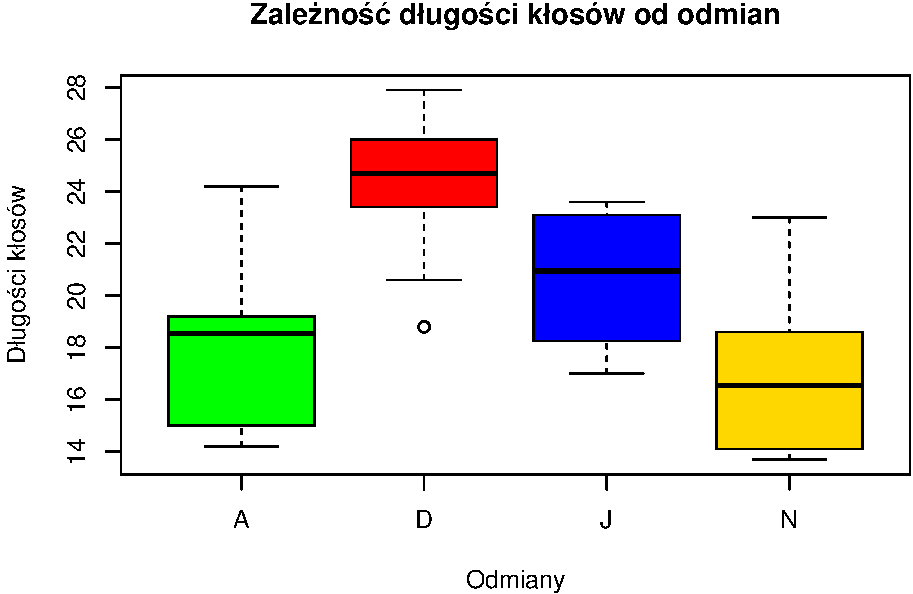
\includegraphics[width=0.7\linewidth]{bookdown-ksiazka_files/figure-latex/unnamed-chunk-93-1} 

}

\caption{Boxploty dla zależność długości kłosów od odmian}\label{fig:unnamed-chunk-93}
\end{figure}

\begin{verbatim}
> # sprawdzamy założenie o normalności
> # rozkładów dla odmian
> shapiro.test(D)
\end{verbatim}

\begin{verbatim}

    Shapiro-Wilk normality test

data:  D
W = 0.94245, p-value = 0.608
\end{verbatim}

\begin{verbatim}
> shapiro.test(A)
\end{verbatim}

\begin{verbatim}

    Shapiro-Wilk normality test

data:  A
W = 0.9408, p-value = 0.5619
\end{verbatim}

\begin{verbatim}
> shapiro.test(J)
\end{verbatim}

\begin{verbatim}

    Shapiro-Wilk normality test

data:  J
W = 0.90125, p-value = 0.2965
\end{verbatim}

\begin{verbatim}
> shapiro.test(N)
\end{verbatim}

\begin{verbatim}

    Shapiro-Wilk normality test

data:  N
W = 0.91073, p-value = 0.2861
\end{verbatim}

\vspace{0.8cm}

\textbf{Interpretacja}

Ponieważ dla wszystkich odmian \(p\)-wartości testu Shapiro--Wilka
(\texttt{shapiro.test}) są większe od 0.05, więc nie odrzucamy hipotezy
\(H_0\), czyli wnioskujemy, że spełniony jest warunek o normalności
rozkładów dla odmian D, A, J i N.

\vspace{0.8cm}

\begin{verbatim}
> # weryfikacja założenia o jednorodności wariancji
> bartlett.test(trawa$Dlugosc,trawa$Odmiany)
\end{verbatim}

\begin{verbatim}

    Bartlett test of homogeneity of variances

data:  trawa$Dlugosc and trawa$Odmiany
Bartlett's K-squared = 0.25106, df = 3, p-value = 0.969
\end{verbatim}

\vspace{0.8cm} \textbf{Interpretacja}

Ponieważ \(p\)-wartość = 0.969, zatem warunek jednorodności wariancji
jest spełniony. Możemy wykonać analizę wariancji.

\vspace{0.8cm}

\begin{verbatim}
> # ANOVA
> model = aov(Dlugosc~Odmiany, trawa)
> summary(model)
\end{verbatim}

\begin{verbatim}
            Df Sum Sq Mean Sq F value   Pr(>F)    
Odmiany      3  291.7   97.22   11.25 3.07e-05 ***
Residuals   33  285.3    8.64                     
---
Signif. codes:  0 '***' 0.001 '**' 0.01 '*' 0.05 '.' 0.1 ' ' 1
\end{verbatim}

\vspace{0.8cm} \textbf{Interpretacja}

Ponieważ \(p\)-wartość \textless{} 0.05, więc odrzucamy hipotezę \(H_0\)
i przyjmujemy \(H_1\). Długości kłosów czterech odmian uprawnych D, A, J
i N badanej trawy różnią się statystycznie istotnie.

\newpage

\textbf{Uwaga}

Ponieważ odrzuciliśmy hipotezę zerową \(H_0\) i przyjęliśmy hipotezę
alternatywną \(H_1\), więc możemy zastosować testy wielokrotne, np. test
Tukeya, aby zbadać istotność różnic wszystkich możliwych par badanych
odmian.

\section{Testy wielokrotne}\label{testy-wielokrotne}

Najczęściej stosowane testy wielokrotne:

\begin{enumerate}
\def\labelenumi{\arabic{enumi}.}
\tightlist
\item
  Test HSD Tukeya (Honestly Significant Differences)
\item
  Test LSD Fishera (Least Significant Differences) -- NIR: Najmniejsza
  Istotna Różnica
\item
  Test Scheffego
\item
  Test Duncana
\item
  Test Newmana-Keulsa
\item
  Test Dunnetta
\end{enumerate}

\vspace{0.8cm} \textbf{Uwagi}

\begin{enumerate}
\def\labelenumi{\arabic{enumi}.}
\item
  Test Tukeya jest bardziej konserwatywny (ostrożny, rzadziej odrzuca
  \(H_0\)) niż test Fishera, a test Fishera jest bardziej konserwatywny
  niż test Scheffego.
\item
  Test Tukeya jest preferowany i najczęściej stosowany, ponieważ mamy
  zagwarantowany poziom istotności \(\alpha\) dla wszystkich
  porównywanych par.
\end{enumerate}

W manuskrypcie zostanie zastosowany test Tukeya.

\vspace{0.8cm}

\textbf{Kod w R}

\begin{verbatim}
# cd. przykładu 5.6 testowanie szczegółowe - test wielokrotny Tukeya
library(agricolae)  # aktywowanie pakietu agricolae
a = HSD.test(model, "Odmiany")  # funkcja z pakietu agricolae
a
# mała litera oznacza grupę odmian podobnych tj. do tej samej grupy należy
# odmiana D i J, innej grupy J i A oraz kolejnej A i N
TukeyHSD(model, "Odmiany", ordered = TRUE)  # funkcja z pakietu stats
plot(TukeyHSD(model, "Odmiany"))  # Rys. 5.4
\end{verbatim}

\vspace{0.8cm} \textbf{Realizacja w R}

\begin{verbatim}
> # cd. przykładu 5.6 testowanie szczegółowe - test wielokrotny Tukeya
> library(agricolae)  # aktywowanie pakietu agricolae
> a = HSD.test(model, "Odmiany")  # funkcja z pakietu agricolae
> a
\end{verbatim}

\begin{verbatim}
$statistics
  MSerror Df     Mean       CV
  8.64434 33 19.78919 14.85723

$parameters
   test  name.t ntr StudentizedRange alpha
  Tukey Odmiany   4         3.825373  0.05

$means
   Dlugosc      std  r  Min  Max    Q25   Q50    Q75
A 18.15000 3.140860 10 14.2 24.2 15.450 18.55 19.200
D 24.14444 2.912950  9 18.8 27.9 23.400 24.70 26.000
J 20.65000 2.618069  8 17.0 23.6 18.375 20.95 22.900
N 16.82000 2.992880 10 13.7 23.0 14.375 16.55 18.175

$comparison
NULL

$groups
   Dlugosc groups
D 24.14444      a
J 20.65000     ab
A 18.15000     bc
N 16.82000      c

attr(,"class")
[1] "group"
\end{verbatim}

\begin{verbatim}
> # mała litera oznacza grupę odmian podobnych tj. do tej samej grupy należy
> # odmiana D i J, innej grupy J i A oraz kolejnej A i N
> TukeyHSD(model, "Odmiany", ordered = TRUE)  # funkcja z pakietu stats
\end{verbatim}

\begin{verbatim}
  Tukey multiple comparisons of means
    95% family-wise confidence level
    factor levels have been ordered

Fit: aov(formula = Dlugosc ~ Odmiany, data = trawa)

$Odmiany
        diff         lwr       upr     p adj
A-N 1.330000 -2.22663884  4.886639 0.7438813
J-N 3.830000  0.05761484  7.602385 0.0455162
D-N 7.324444  3.67034540 10.978543 0.0000304
J-A 2.500000 -1.27238516  6.272385 0.2948589
D-A 5.994444  2.34034540  9.648543 0.0005319
D-J 3.494444 -0.36996363  7.358853 0.0879854
\end{verbatim}

\begin{verbatim}
> plot(TukeyHSD(model, "Odmiany"))  # Rys. 5.4
\end{verbatim}

\begin{figure}[H]

{\centering 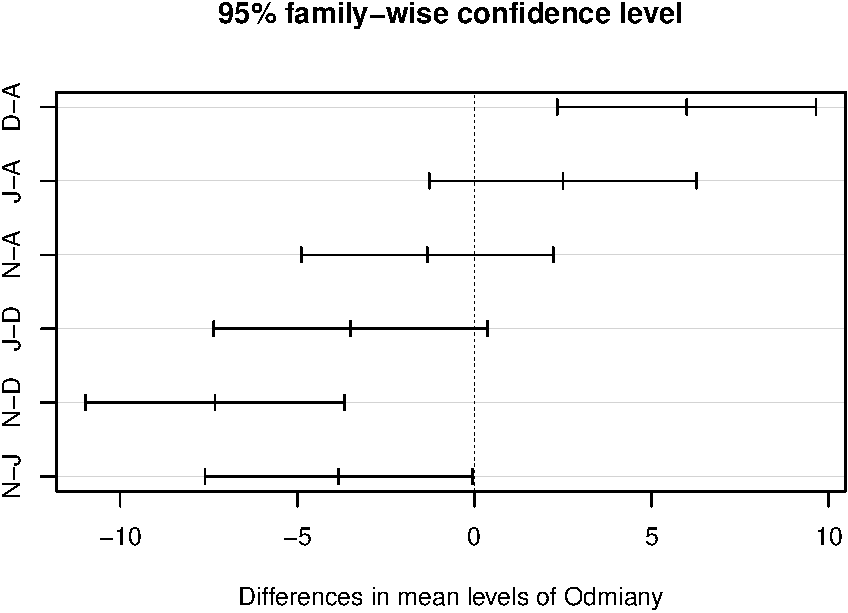
\includegraphics[width=0.7\linewidth]{bookdown-ksiazka_files/figure-latex/unnamed-chunk-97-1} 

}

\caption{Graficzne przedstawienie porównań wielokrotnych.}\label{fig:unnamed-chunk-97}
\end{figure}

Rysunek 5.4 przedstawia porównania odmian parami. Dla odmian, które nie
różnią się istotnie statystycznie odcinki na wykresie przechodzą przez
punkt zero, natomiast dla odmian różniących się istotnie statystycznie
odcinki nie przechodzą przez punkt zero.

Poniżej w formie tabel (patrz Tablica \ref{pwartosci}) przedstawione są
trzy sposoby prezentacji porównań wielokrotnych.

\begin{table}[H]
\centering
\caption{Porównania pomiędzy odmianami (p-wartości)}
\label{pwartosci}
\begin{tabular}{cccc}
  & A                                & J         & N                                \\ \hline
D & {\color[HTML]{FE0000} 0.0005319} & 0.0879854 & {\color[HTML]{FE0000} 0.0000304} \\
A &                                  & 0.2948589 & 0.7438813                        \\
J &                                  &           & {\color[HTML]{FE0000} 0.0455162} \\ \hline
\end{tabular}
\end{table}

lub

\begin{table}[H]
\centering
\begin{tabular}{cccc}
  & A                                & J         & N                                \\ \hline
D & {\color[HTML]{FE0000} x} & ns & {\color[HTML]{FE0000} x} \\
A &                                  & ns & ns                        \\
J &                                  &           & {\color[HTML]{FE0000} x} \\ \hline
\end{tabular}
\end{table}

\textcolor{red}{x} - statystycznie istotna różnica, ns -- nie ma różnicy

lub

\begin{table}[H]
\centering
\begin{tabular}{cc}
Odmiany & Średnie* \\ \hline
D       & $24.14^a$  \\
J       & $20.65^{ab}$  \\
A       & $18.25^{bc}$  \\
N       & $16.82^c$   \\ \hline
\end{tabular}
\end{table}

\(\ast\) mała litera (indeks górny) oznacza grupę odmian podobnych.

\newpage

\textbf{Przykład 5.7} (Greń 1975, s. 105)

Ceny jednego kwiatu róży ogrodowej na trzech różnych targowiskach były
następujące (w zł):

\begin{table}[H]
\centering
\caption{Dane - Greń (1975, s. 105)}
\label{gren105}
\begin{tabular}{ccc}
\hline
\multicolumn{3}{c}{Miasto} \\ \hline
A        & B      & C      \\ \hline
10       & 3      & 2      \\
7        & 4      & 8      \\
3        & 2      & 5      \\
11       & 4      & 6      \\
9        & 5      & 3      \\
10       &       & 6      \\
15       &       &       \\
5        &       &      \\ \hline
\end{tabular}
\end{table}

Zweryfikować hipotezę, że targowiska we wszystkich trzech miastach nie
różnią się średnimi cenami kwiatu róży.

\vspace{0.8cm} \textbf{Kod w R}

\begin{verbatim}
# Przykład 5.7 (Greń 1975, s. 105)
# wprowadzamy dane
A = c(10,7,3,11,9,10,15,5)
B = c(3,4,2,4,5)
C = c(2,8,5,6,3,6)
# sprawdzamy założenie o normalności rozkładów 
shapiro.test(A)
shapiro.test(B)
shapiro.test(C)
# przygotowanie danych w formie ramki danych
kwiat=data.frame(Ceny=c(A, B, C), Miasto=c(rep('A',8),rep('B',5),rep('C',6)))
head(kwiat)
# weryfikacja założenia o jednorodności wariancji - test Bartleta
bartlett.test(kwiat$Ceny,kwiat$Miasto)
# ANOVA
model=aov(Ceny~Miasto, data=kwiat)
summary(model)
\end{verbatim}

\vspace{0.8cm}

\textbf{Realizacja w R}

\begin{verbatim}
> # Przykład 5.7 (Greń 1975, s. 105)
> # wprowadzamy dane
> A = c(10,7,3,11,9,10,15,5)
> B = c(3,4,2,4,5)
> C = c(2,8,5,6,3,6)
> # sprawdzamy założenie o normalności rozkładów 
> shapiro.test(A)
\end{verbatim}

\begin{verbatim}

    Shapiro-Wilk normality test

data:  A
W = 0.97307, p-value = 0.921
\end{verbatim}

\begin{verbatim}
> shapiro.test(B)
\end{verbatim}

\begin{verbatim}

    Shapiro-Wilk normality test

data:  B
W = 0.96086, p-value = 0.814
\end{verbatim}

\begin{verbatim}
> shapiro.test(C)
\end{verbatim}

\begin{verbatim}

    Shapiro-Wilk normality test

data:  C
W = 0.95529, p-value = 0.7828
\end{verbatim}

\vspace{0.8cm} \textbf{Interpretacja}

Wszystkie \(p\)-wartości \textgreater{} 0.05, więc \(H_0\) nie odrzucamy
co oznacza, że próby pochodzą z rozkładu normalnego.

\vspace{0.8cm}

\begin{verbatim}
> # przygotowanie danych w formie ramki danych
> kwiat=data.frame(Ceny=c(A, B, C), Miasto=c(rep('A',8),rep('B',5),rep('C',6)))
> head(kwiat)
\end{verbatim}

\begin{verbatim}
  Ceny Miasto
1   10      A
2    7      A
3    3      A
4   11      A
5    9      A
6   10      A
\end{verbatim}

\begin{verbatim}
> # weryfikacja założenia o jednorodności wariancji - test Bartleta
> bartlett.test(kwiat$Ceny,kwiat$Miasto)
\end{verbatim}

\begin{verbatim}

    Bartlett test of homogeneity of variances

data:  kwiat$Ceny and kwiat$Miasto
Bartlett's K-squared = 5.3084, df = 2, p-value = 0.07036
\end{verbatim}

\vspace{0.8cm} \textbf{Interpretacja}

Ponieważ \(p\)-wartość = 0.07036 \textgreater{} 0.05, więc nie odrzucamy
\(H_0\), a to oznacza, że założenie o jednorodności wariancji jest
spełnione - możemy zatem wykonać analizę wariancji ANOVA.

\vspace{0.8cm}

\begin{verbatim}
> # ANOVA
> model=aov(Ceny~Miasto, data=kwiat)
> summary(model)
\end{verbatim}

\begin{verbatim}
            Df Sum Sq Mean Sq F value Pr(>F)  
Miasto       2  94.46   47.23   5.964 0.0116 *
Residuals   16 126.70    7.92                 
---
Signif. codes:  0 '***' 0.001 '**' 0.01 '*' 0.05 '.' 0.1 ' ' 1
\end{verbatim}

\vspace{0.8cm} \textbf{Interpretacja}

Ponieważ \(p\)-wartość = 0.0116 \textless{} 0.05, więc odrzucamy \(H_0\)
i przyjmujemy \(H_1\), czyli we wszystkich trzech miastach ceny kwiatu
róży różnią się. Następnie stosujemy test Tukeya, aby zbadać istotność
różnic pomiędzy średnimi cenami kwiatu róży we wszystkich miastach.
\vspace{0.8cm}

\textbf{Kod w R}

\begin{verbatim}
# testowanie szczegółowe - test wielokrotny Tukeya
a=HSD.test(model,"Miasto")
a
TukeyHSD(model,"Miasto", ordered = TRUE)  
plot(TukeyHSD(model,"Miasto")) # Rys. 5.5
\end{verbatim}

\vspace{0.8cm} \textbf{Realizacja w R}

\begin{verbatim}
> # testowanie szczegółowe - test wielokrotny Tukeya
> a=HSD.test(model,"Miasto")
> a
\end{verbatim}

\begin{verbatim}
$statistics
  MSerror Df     Mean       CV
  7.91875 16 6.210526 45.31061

$parameters
   test name.t ntr StudentizedRange alpha
  Tukey Miasto   3         3.649139  0.05

$means
  Ceny      std r Min Max Q25 Q50   Q75
A 8.75 3.732100 8   3  15 6.5 9.5 10.25
B 3.60 1.140175 5   2   5 3.0 4.0  4.00
C 5.00 2.190890 6   2   8 3.5 5.5  6.00

$comparison
NULL

$groups
  Ceny groups
A 8.75      a
C 5.00     ab
B 3.60      b

attr(,"class")
[1] "group"
\end{verbatim}

\begin{verbatim}
> TukeyHSD(model,"Miasto", ordered = TRUE)  
\end{verbatim}

\begin{verbatim}
  Tukey multiple comparisons of means
    95% family-wise confidence level
    factor levels have been ordered

Fit: aov(formula = Ceny ~ Miasto, data = kwiat)

$Miasto
    diff        lwr      upr     p adj
C-B 1.40 -2.9968275 5.796827 0.6954262
A-B 5.15  1.0105238 9.289476 0.0142703
A-C 3.75 -0.1714539 7.671454 0.0620108
\end{verbatim}

\begin{verbatim}
> plot(TukeyHSD(model,"Miasto")) # Rys. 5.5
\end{verbatim}

\begin{figure}[H]

{\centering 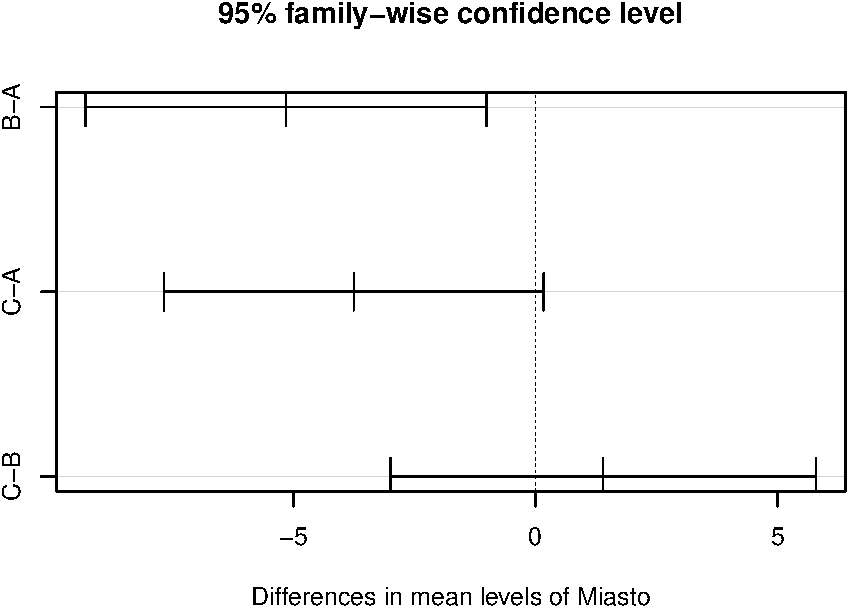
\includegraphics[width=0.7\linewidth]{bookdown-ksiazka_files/figure-latex/unnamed-chunk-103-1} 

}

\caption{Graficzne przedstawienie porównań wielokrotnych}\label{fig:unnamed-chunk-103}
\end{figure}

\textbf{Interpretacja}

Dla porównania pomiędzy miastami A i B \(p\)-wartość = 0.0142703 i jest
ona mniejsza od 0.05, zatem dla tych miast wykazano istotne różnice w
średnich cenach kwiatu róży. Ten sam wniosek wynika z analizy wykresu
5.5, gdzie tylko dla porównania odmian A i B odcinki na wykresie nie
przechodzą przez punkt zero, co oznacza, że różnią się istotnie.

\section{Zadania do wykonania}\label{zadania-do-wykonania-4}

\textbf{Testy dwóch wartości średnich z rozkładów normalnych - próby
zależne}

Zad. 1 (Elandt 1964, str. 104)

Dane są średnie wyniki długości technicznej słomy lnianej 4 odmian lnu
włóknistego odpowiednio w latach 1948 i 1949 w tej samej miejscowości.
Czy można stwierdzić wpływ warunków meteorologicznych na długość słomy
lnianej?

\begin{table}[H]
\centering
\caption{Dane - Elandt (1964, str. 104)}
\label{elandt104}
\begin{tabular}{ccc}
\hline
Odmiana/Lata & 1948 ($x_1$) & 1949 ($x_2$) \\ \hline
1            & 68.9      & 64.5      \\
2            & 52.6      & 54.8      \\
3            & 59.5      & 57.9      \\
4            & 60.3      & 57.2      \\ \hline
\end{tabular}
\end{table}

Zad. 2 (Dobek, Szwaczkowski 2007, str. 90)

Badano wpływ sposobu rozmnażania pewnej rośliny uprawnej na długość
pędów. W tym celu na każdym z ośmiu poletek umieszczono rośliny
samopylne i pochodzące z krzyżowania, uzyskując następujące wyniki:

\begin{table}[H]
\centering
\caption{Dane - Dobek, Szwaczkowski (2007, str. 90)}
\label{Dobek90}
\begin{tabular}{ccccccccc}
\hline
Nr poletka  & 1   & 2   & 3   & 4   & 5  & 6  & 7   & 8   \\ \hline
Krzyżowanie & 188 & 101 & 156 & 197 & 97 & 94 & 120 & 178 \\
Samopylność & 150 & 97  & 134 & 139 & 95 & 91 & 118 & 161 \\ \hline
\end{tabular}
\end{table}

Zauważmy, że każda grupa roślin z danego poletka ma identyczne warunki
glebowe, stąd możemy przyjąć zależność obydwu grup roślin. Zweryfikować
hipotezę zerową mówiącą o tym, że różnice między wysokością roślin z
poszczególnych poletek są takie same.

\vspace{0.8cm}

\textbf{Analiza wariancji - ANOVA}

Zad. 1 (Elandt 1964, str. 155)

Zastosowano 4 terminy cięcia łubinu białego na zielonkę. Doświadczenie
przeprowadzono na polu gospodarczym wycinając w różnych miejscach po 8
poletek wielkości 9 \(m^2\). Wyniki zestawiono w Tablicy
\ref{elandt155}.

\begin{table}[H]
\centering
\caption{Dane - Elandt (1964, str. 155)}
\label{elandt155}
\begin{tabular}{ccccc}
\hline
\multirow{2}{*}{Powtórzenia} & \multicolumn{4}{c}{Terminy}   \\ 
                             & I     & II    & III   & IV    \\ \hline
1                            & 290   & 445   & 520   & 370   \\
2                            & 286   & 450   & 470   & 405   \\
3                            & 266   & 413   & 516   & 412   \\
4                            & 270   & 448   & 530   & 403   \\
5                            & 301   & 454   & 475   & 384   \\
6                            & 270   & 442   & 508   & 410   \\
7                            & 264   & 430   & 485   & 415   \\
8                            & 277   & 438   & 480   & 377   \\  \hline
\end{tabular}
\end{table}

Sprawdź, czy istnieje wpływ terminu w którym cięty był łubin biały na
plon zielonki łubinu.

\vspace{0.8cm} Zad. 2 (Kala 2005, s. 158)

W doświadczeniu z czterema odmianami kukurydzy S, L, A, D określono masę
tysiąca ziaren (w g):

\begin{table}[H]
\centering
\caption{Dane - Kala (2005, s. 158)}
\label{kala158}
\begin{tabular}{ccccc}
\hline
& \multicolumn{4}{c}{Replikacja}   \\  \hline
S & 214.6 & 193.1 & 189.1 & 177.7 \\
L & 262.3 & 235.9 & 216.5 & 219.1 \\
A & 221.4 & 236.8 & 227.9 & 234.1 \\
D & 248.0 & 255.0 & 229.6 & 242.8 \\ \hline
\end{tabular}
\end{table}

Czy badane odmiany różni przeciętna masa tysiąca ziaren? Przyjąć, że
\(\alpha\) = 0.05.

\vspace{0.8cm}

\textbf{Testy wielokrotne}

Zad. 1 (Dobek, Szwaczkowski 2007, s. 124)

Badano zawartość fenolu (w mg/litr wody) w siedmiu jeziorach
zróżnicowanych pod względem położenia względem ośrodka przemysłowego.
Pierwsze z jezior (L1) leży w jego bezpośrednim sąsiedztwie. Kolejne
jeziora (L2, L3,\ldots{}, L7) leżą średnio w odległości co ok. 2 km od
poprzedniego, w stronę przeciwną do centrum przemysłowego. Z każdego ze
zbiorników pobrano pięć próbek wody w pięciu kolejnych miesiącach,
uzyskując następujące wyniki:

\begin{table}[H]
\centering
\caption{Dane - Dobek, Szwaczkowski (2007, s. 124)}
\label{dobek124}
\begin{tabular}{cccccc}
\hline
\multirow{2}{*}{Jezioro} & \multicolumn{5}{c}{Replikacja}   \\
                         & 1    & 2    & 3    & 4    & 5    \\ \hline
L1                       & 0.26 & 0.28 & 0.27 & 0.25 & 0.19 \\
L2                       & 0.30 & 0.27 & 0.26 & 0.22 & 0.19 \\
L3                       & 0.26 & 0.25 & 0.24 & 0.22 & 0.20 \\
L4                       & 0.25 & 0.23 & 0.21 & 0.22 & 0.21 \\
L5                       & 0.23 & 0.22 & 0.22 & 0.21 & 0.20 \\
L6                       & 0.21 & 0.21 & 0.20 & 0.20 & 0.20 \\
L7                       & 0.24 & 0.22 & 0.21 & 0.20 & 0.18 \\ \hline
\end{tabular}
\end{table}

Spawdzić, czy słuszne jest przypuszczenie, że stężenie fenolu zależy od
miejsca położenia jeziora.

\vspace{0.8cm} Zad. 2 (Kala 2005, s. 167)

Badając w doświadczeniu wazonowym wpływ nawożenia mineralnego na plon
olejku w zielu cząbru ogrodowego, uzyskano dla 6 kombinacji nawozowych i
kontroli następujące obserwacje (w ml/wazon):

\begin{table}[H]
\centering
\caption{Dane - (Kala 2005, s. 167)}
\label{Kala167}
\begin{tabular}{ccccccc}
\hline
K    & N1   & N2   & N3   & N4   & N5   & N6   \\ \hline
0.16 & 0.18 & 0.62 & 0.62 & 0.29 & 0.39 & 0.61 \\
0.23 & 0.28 & 0.38 & 0.68 & 0.24 & 0.37 & 0.65 \\
0.39 & 0.39 & 0.63 & 0.63 & 0.20 & 0.49 & 0.57 \\
0.34 & 0.16 & 0.52 & 0.52 & 0.26 & 0.44 & 0.67 \\
0.23 & 0.48 & 0.61 & 0.61 & 0.18 & 0.47 & 0.69 \\
0.38 & 0.44 & 0.57 & 0.57 & 0.19 & 0.53 & 0.65 \\ \hline
\end{tabular}
\end{table}

Czy wszystkie badane kombinacje nawozowe zapewniają taki sam plon
olejku?

\chapter{Badanie zależności cech}\label{badanie-zaleznosci-cech}

\section{Korelacje}\label{korelacje}

Korelacja wskazuje siłę i kierunek zależności pomiędzy dwiema cechami.
Korelacja dla próby wyrażona jest za pomocą współczynnika korelacji
\(r\), gdzie \(r \in \langle -1; 1 \rangle\).

\vspace{0.8cm}

Interpretacja współczynnika korelacji \(r\):

\(|r| = 0\) - brak korelacji,

\(0,0 < |r| \leq 0,1\) - korelacja nikła,

\(0,1 < |r| \leq 0,3\) - korelacja słaba,

\(0,3 < |r| \leq 0,5\) - korelacja przeciętna,

\(0,5 < |r| \leq 0,7\) - korelacja wysoka,

\(0,7 < |r| \leq 0,9\) - korelacja bardzo wysoka,

\(0,9 < |r| < 1,0\) - korelacja niemal pełna (silna),

\(|r| = 1\) - korelacja pełna (bardzo silny związek liniowy).

\vspace{0.8cm}

Jeśli wartość współczynnika korelacji \(r\) jest dodatnia to mamy
zależność liniową dodatnią. Oznacza to, że wraz ze wzrostem wartości
jednej cechy rosną wartości drugiej cechy. Natomiast, jeśli wartość
współczynnika korelacji \(r\) jest ujemna to mamy zależność liniową
ujemną, tzn. wraz ze wzrostem wartości jednej cechy maleją wartości
drugiej cechy.

\vspace{0.8cm}

\textbf{Uwaga}

Oprócz wyznaczania wartości współczynnika korelacji \(r\) dla próby,
należy zawsze zbadać czy współczynnik korelacji dla populacji jest
istotny. Weryfikację hipotez o istotności współczynnika korelacji dla
populacji możemy wykonać przy pomocy funkcji
\texttt{cor.test(x, y, method='aaa')}, gdzie `aaa'=`pearson' lub
`kendall' lub `spearman' oraz domyślnie `aaa'=`pearson'.

\subsection{Cechy ilościowe}\label{cechy-ilosciowe}

Cecha ilościowa (mierzalna) jest to cecha, która przyjmuje wartości
liczbowe. Dla cech ilościowych (np. cechy x i cechy y) wyznacza się
współczynnik korelacji \(r\) Pearsona stosując funkcję
\texttt{cor(x, y)}. Natomiast istotność współczynnika korelacji
testujemy funkcją \texttt{cor.test(x, y)} lub
\texttt{cor.test(x, y, method='pearson')}.

\vspace{0.8cm} \textbf{Przykład 6.1} (Dobek, Szwaczkowski 2007, s. 153)

Badano zależność pomiędzy długością pędu (cm) a długością kłosa (cm)
pewnej odmiany pszenicy. Z poletka wybrano losowo 25 roślin, u których
dokonano pomiaru obydwu cech. Wyniki zaprezentowano w Tablicy
\ref{Dobek}.

\begin{table}[!ht]
\centering
\caption{Dane - Dobek, Szwaczkowski (2007, s. 153)}
\label{Dobek}
\begin{tabular}{ccc|ccc}
\hline
\begin{tabular}[c]{@{}c@{}}numer \\ rośliny\end{tabular} & \begin{tabular}[c]{@{}c@{}}długość pędu \\ (cm)\end{tabular} & \begin{tabular}[c]{@{}c@{}}długość kłosa \\ (cm)\end{tabular} & \begin{tabular}[c]{@{}c@{}}numer \\ rośliny\end{tabular} & \begin{tabular}[c]{@{}c@{}}długość pędu\\  (cm)\end{tabular} & \begin{tabular}[c]{@{}c@{}}długość kłosa\\  (cm)\end{tabular} \\ \hline
nr & dp   & dk   & nr & dp  & dk   \\ \hline
1 & 105  & 5.6   & 14 & 107 & 6.6  \\
2  & 103  & 6.2  & 15 & 106 & 6.4  \\
3  & 101  & 4.8  & 16 & 102 & 5.0  \\
4 & 107  & 6.5  & 17  & 100 & 4.9  \\
5 & 103 & 5.4 & 18  & 100   & 5.0   \\
6  & 102  & 5.0  & 19  & 106  & 6.0  \\
7  & 104  & 5.6  & 20  & 105  & 4.9   \\
8 & 103  & 6.0  & 21  & 105  & 4.8   \\
9  & 102 & 4.9   & 22  & 101  & 5.2   \\
10  & 106 & 6.3  & 23  & 105  & 4.8   \\
11 & 105  & 5.2  & 24  & 101 & 5.1  \\
12  & 101  & 4.9  & 25  & 101  & 5.0  \\
13  & 103  & 5.3  &  &   &  \\ \hline                         
\end{tabular}
\end{table}

Czy korelacja między badanymi cechami jest istotna?

\vspace{0.8cm} \textbf{Kod w R}

\begin{verbatim}
# Przykład 6.1 (Dobek, Szwaczkowski 2007, s. 153)
# usuwanie wszystkich zmiennych z przestrzeni roboczej
rm(list=ls()) 
# tworzenie danych
pszenica=read.table("~/Desktop/Dobek_153.txt",header=T)
head(pszenica)
# funkcja round wyświetla wyniki z zaokrągleniem do 2 miejsc po przecinku
round(cor(pszenica$dk,pszenica$dp),2)  
# testowanie istotności korelacji
cor.test(pszenica$dk,pszenica$dp)
\end{verbatim}

\newpage

\textbf{Realizacja w R}

\begin{verbatim}
> # Przykład 6.1 (Dobek, Szwaczkowski 2007, s. 153)
> # usuwanie wszystkich zmiennych z przestrzeni roboczej
> rm(list=ls()) 
> # tworzenie danych
> pszenica=read.table("~/Desktop/Dobek_153.txt", header=T)
> head(pszenica)
\end{verbatim}

\begin{verbatim}
  nr  dp  dk
1  1 105 5.6
2  2 103 6.2
3  3 101 4.8
4  4 107 6.5
5  5 103 5.4
6  6 102 5.0
\end{verbatim}

\begin{verbatim}
> # funkcja round wyświetla wyniki z zaokrągleniem do 2 miejsc po przecinku
> round(cor(pszenica$dk,pszenica$dp),2)  
\end{verbatim}

\begin{verbatim}
[1] 0.66
\end{verbatim}

\begin{verbatim}
> # testowanie istotności korelacji
> cor.test(pszenica$dk,pszenica$dp)
\end{verbatim}

\begin{verbatim}

    Pearson's product-moment correlation

data:  pszenica$dk and pszenica$dp
t = 4.2547, df = 23, p-value = 0.0002984
alternative hypothesis: true correlation is not equal to 0
95 percent confidence interval:
 0.3639564 0.8388175
sample estimates:
      cor 
0.6636478 
\end{verbatim}

\vspace{0.8cm} \textbf{Interpretacja}

Wartość współczynnika korelacji \(r\) Pearsona wynosi 0,66, więc
korelacja jest wysoka. Ponadto, ponieważ \(p\)-wartość = 0,0003, więc
odrzucamy hipotezę zerową i przyjmujemy hipotezę alternatywną
stwierdzając, że zależność pomiędzy długością pędu a długością kłosa
pewnej odmiany pszenicy jest istotna.

\subsection{Cechy jakościowe}\label{cechy-jakosciowe}

Cecha jakościowa (niemierzalna) jest to cecha, która ma charakter
opisowy lub podlega kategoryzacji. Współczynnik korelacji \(r_S\)
Spearmana używamy w przypadku gdy:

\begin{enumerate}
\def\labelenumi{\arabic{enumi}.}
\item
  choć jedna z badanych cech jest cechą jakościową (niemierzalną), ale
  istnieje możliwość uporządkowania (ponumerowania) wariantów każdej z
  cech,
\item
  cechy mają charakter ilościowy (mierzalny), ale liczebność zbiorowości
  jest mała (n\textless{}30).
\end{enumerate}

\vspace{0.8cm} \textbf{Przykład 6.2} (Dobek, Szwaczkowski 2007, s. 163)

Dwaj eksperci niezależnie oceniali stopień porażenia ziarniaków w skali
od 1 do 20. Uzyskali następujące wyniki:

ekspert 1: 5, 7, 34, 9, 12, 16, 9, 13, 18, 6, 17

ekspert 2: 6, 6, 3, 10, 8, 18, 10, 11, 16, 8, 15

Czy oceny obu ekspertów są skorelowane?

\newpage

\textbf{Kod w R}

\begin{verbatim}
# Przykład 6.2 (Dobek, Szwaczkowski 2007, s. 153)
eksp1=c(5, 7, 34, 9, 12, 16, 9, 13, 18, 6, 17)
eksp2=c(6, 6, 3, 10, 8, 18, 10, 11, 16, 8, 15)
cor.test(eksp1, eksp2, method = "spearman")
\end{verbatim}

\vspace{0.8cm} \textbf{Realizacja w R}

\begin{verbatim}
> # Przykład 6.2 (Dobek, Szwaczkowski 2007, s. 153)
> eksp1=c(5, 7, 34, 9, 12, 16, 9, 13, 18, 6, 17)
> eksp2=c(6, 6, 3, 10, 8, 18, 10, 11, 16, 8, 15)
> cor.test(eksp1, eksp2, method = "spearman")
\end{verbatim}

\begin{verbatim}

    Spearman's rank correlation rho

data:  eksp1 and eksp2
S = 130.18, p-value = 0.2126
alternative hypothesis: true rho is not equal to 0
sample estimates:
      rho 
0.4082612 
\end{verbatim}

\vspace{0.8cm} \textbf{Interpretacja}

Wartość współczynnika korelacji Spearmana \(r_S=0,408\), więc korelacja
jest przeciętna. Ponadto, ponieważ \(p\)-wartość=0,2126, więc nie
odrzucamy hipotezy zerowej i stwierdzamy, że współczynnik korelacji
Spearmana nie różni się istotnie od zera. Oznacza to, że oceniani
eksperci niezależnie ocenili stopień porażenia ziarniaków.

\section{Tablice kontyngencji}\label{tablice-kontyngencji}

Tablica kontyngencji przedstawia liczebności dwóch cech (zmiennych)
jakościowych (niemierzalnych). Najczęściej interesujące są następujące
hipotezy:

\hspace*{5cm} \(H_0\): cechy \(X\) i \(Y\) są niezależne

\hspace*{5cm} \(H_1\): cechy \(X\) i \(Y\) są zależne \hfill (6.1)

Weryfikację hipotez (6.1) wykonuje się stosując test \(\chi^2\)
(\texttt{chisq.test}). Jeśli conajmniej jedna liczebność ma wartość 5
lub mniej, to należy zastosować dokładny test Fishera
(\texttt{fisher.test}).

\vspace{0.8cm} \textbf{Przykład 6.3} (Kala 2005, s. 87)

Badając jakość jabłek oceniono owoce ze względu na uszkodzenia
spowodowane przez owocówkę jabłkóweczkę (U - owoce uszkodzone, N - owoce
nieuszkodzone) oraz porażone parchem jabłoniowym (C - owoce czyste, P -
owoce z plamami). W wyniku klasyfikacji owoców uzyskano następujące
liczebności:

\begin{table}[H]
\centering
\caption{Dane - Kala (2005, s. 87)}
\label{Kala}
\begin{tabular}{ccc}
\hline
\multirow{2}{*}{Parch} & \multicolumn{2}{c}{Owocówka} \\
& U            & N             \\ \hline
C      & 29           & 194           \\
P      & 17           & 68      \\ \hline     
\end{tabular}
\end{table}

Czy na poziomie istotności 0,01 można uznać, że badane zmienne są
niezależne?

\vspace{0.8cm} \textbf{Kod w R}

\begin{verbatim}
# Przykład 6.3 (Kala 2005, s. 87)
# analiza tablicy kontyngencji
x = matrix(c(29, 17, 194, 68), ncol = 2)
x
chisq.test(x)
\end{verbatim}

\vspace{0.8cm} \textbf{Realizacja w R}

\begin{verbatim}
> # Przykład 6.3 (Kala 2005, s. 87)
> # analiza tablicy kontyngencji
> x = matrix(c(29, 17, 194, 68), ncol = 2)
> x
\end{verbatim}

\begin{verbatim}
     [,1] [,2]
[1,]   29  194
[2,]   17   68
\end{verbatim}

\begin{verbatim}
> chisq.test(x)
\end{verbatim}

\begin{verbatim}

    Pearson's Chi-squared test with Yates' continuity correction

data:  x
X-squared = 1.8519, df = 1, p-value = 0.1736
\end{verbatim}

\vspace{0.8cm} \textbf{Interpretacja}

Ponieważ \(p\)-wartość = 0.1736, więc nie odrzucamy hipotezy \(H_0\) i
stwierdzamy, że badane zmienne są niezależne.

\vspace{0.8cm} \textbf{Przykład 6.4} (Hanusz, Tarasińska 2006, s. 84)

W celu sprawdzenia, czy przy ocenie stanu technicznego pewnego
urządzenia można się posługiwać łatwym do wyznaczenia pomiarem, wybrano
losowo 100 urządzeń i zanotowano następujące dane:

\begin{table}[H]
\centering
\caption{Dane - Hanusz, Tarasińska (2006, s. 84)}
\label{hanusz}
\begin{tabular}{cccc}
\hline
\multirow{2}{*}{Stan urządzenia} &  \multicolumn{3}{c}{Wartość pomiaru} \\
 & niska     & średnia     & wysoka    \\ \hline
dobry        & 37        & 22          & 11 \\
zły         & 6         & 9           & 15   \\ \hline    
\end{tabular}
\end{table}

\vspace{0.8cm} \textbf{Kod w R}

\begin{verbatim}
# Przykład 6.4 (Hanusz, Tarasińska 2006, s. 84)
x = matrix(c(37, 6, 22, 9, 11, 15), ncol = 3)
x
chisq.test(x)
\end{verbatim}

\vspace{0.8cm} \textbf{Realizacja w R}

\begin{verbatim}
> # Przykład 6.4 (Hanusz, Tarasińska 2006, s. 84)
> x = matrix(c(37, 6, 22, 9, 11, 15), ncol = 3)
> x
\end{verbatim}

\begin{verbatim}
     [,1] [,2] [,3]
[1,]   37   22   11
[2,]    6    9   15
\end{verbatim}

\begin{verbatim}
> chisq.test(x)
\end{verbatim}

\begin{verbatim}

    Pearson's Chi-squared test

data:  x
X-squared = 14.781, df = 2, p-value = 0.0006172
\end{verbatim}

\vspace{0.8cm} \textbf{Interpretacja}

Ponieważ \(p\)-wartość \(= 0.0006172\), więc odrzucamy hipotezę \(H_0\)
i przyjmujemy hipotezę \(H_1\). Stwierdzamy, że ocena stanu badanego
urządzenia zależy od wartości pomiaru.

\vspace{0.8cm} \textbf{Przykład 6.5}

Wysunięto hipotezę, że wadliwość produkcji luksusowych samochodów nie
zależy od metody produkcji. Wylosowano niezależnie próbę 296 aut i
otrzymano następujące wyniki badania jakości dla poszczególnych metod:

\begin{table}[H]
\centering
\caption{Dane do przykładu 6.5}
\label{dane6.4}
\begin{tabular}{cccc}
\hline
\multirow{2}{*}{Jakość} &  \multicolumn{3}{c}{Metoda produkcji} \\
 & I     & II    & III    \\ \hline
dobra        & 5 & 67  & 75 \\
zła         & 4  & 96  & 49   \\ \hline    
\end{tabular}
\end{table}

\vspace{0.8cm} \textbf{Kod w R}

\begin{verbatim}
# Przykład 6.5
x = matrix(c(5,4,67,96,75,49), ncol = 3)
x
fisher.test(x)
\end{verbatim}

\vspace{0.8cm} \textbf{Realizacja w R}

\begin{verbatim}
> # Przykład 6.5
> x = matrix(c(5,4,67,96,75,49), ncol = 3)
> x
\end{verbatim}

\begin{verbatim}
     [,1] [,2] [,3]
[1,]    5   67   75
[2,]    4   96   49
\end{verbatim}

\begin{verbatim}
> fisher.test(x)
\end{verbatim}

\begin{verbatim}

    Fisher's Exact Test for Count Data

data:  x
p-value = 0.004014
alternative hypothesis: two.sided
\end{verbatim}

\vspace{0.8cm} \textbf{Interpretacja}

Ponieważ \(p\)-wartość=0.004014, więc odrzucamy hipotezę \(H_0\) i
przyjmujemy hipotezę \(H_1\). Stwierdzamy, że wadliwość produkcji
luksusowych samochodów nie zależy od metody produkcji.

\section{Zadania do wykonania}\label{zadania-do-wykonania-5}

\textbf{Korelacje}

Zad. 1 (Dobek, Szwaczkowski 2007, s. 163)

U dziewięciu losowo wybranych koni półkrwi dokonano pomiaru wysokości w
kłębie (cm) i obwodu nadpęcia (cm), uzyskując następujące wyniki:

wysokość w kłębie: 163, 170, 158, 156, 161, 159, 161, 168, 177

obwód nadpęcia: 21, 24, 22, 19, 24, 26, 26, 27, 28

Sprawdź, czy cechy te są skorelowane.

\vspace{0.8cm} Zad. 2 (Dobek, Szwaczkowski 2007, s. 163)

W badaniach nad strukturą plonu pszenżyta, przy gęstości wysiewu 400
ziaren/\(m^2\), oznaczono masę 1000 ziaren i plon ziarna. Uzyskano
następujące obserwacje:

masa 1000 ziaren: 44.1, 45.6, 45.2, 46.8, 43.3, 47.1, 46.8, 45.7

plon: 4.68, 4.76, 4.71, 4.87, 4.31, 4.97, 4.82, 4.72

Czy korelacja między badanymi cechami jest istotna?

\vspace{0.8cm}

\textbf{Tablice kontyngencji}

Zad. 1 (Greń 1975, s. 138)

W pewnym doświadczeniu farmakologicznym otrzymano na 120 badanych
szczurów, którym podano pewien preparat, 57 takich, które doszły do
pokarmu w labiryncie doświadczalnym w czasie do 1 minuty. Natomiast na
100 szczurów, którym nie podano tego preparatu, 71 wykonało to zadanie w
tym samym czasie. Sporządzono następującą tablicę wyników badania
farmakologicznego:

\begin{table}[H]
\centering
\caption{Dane - Greń (1975, s. 138)}
\label{gren138}
\begin{tabular}{ccc}
\hline
liczba szczurów      & z preparatem & bez preparatu \\ \hline
wykonały zadanie     & 57           & 71            \\
nie wykonały zadania & 63           & 19            \\ \hline
\end{tabular}
\end{table}

Zweryfikuj hipotezę o otępiającym działaniu badanego preparatu.

\vspace{0.8cm} Zad. 2 (Greń 1975, s. 135)

Wysunięto hipotezę medyczną, że pacjenci z objawem klinicznym
niewydolności oddechowej charaktarezują się istotnie zawyżonym poziomem
aktywności pewnego enzymu. Losowa próba 49 pacjentów z niewydolnością
oddechową i 208 pacjentów bez objawów tej niewydolności dały wyniki
zestawione w Tablicy \ref{gren135}. Na poziomie istotności 0.01
zweryfikować hipotezę o niezależności aktywności badanego enzymu w
organiźmie chorych od posiadania objawu klinicznego niewydolności
oddechowej.

\begin{table}[H]
\centering
\caption{Dane - Greń (1975, s. 135)}
\label{gren135}
\begin{tabular}{ccc}
\hline
\multirow{2}{*}{Niewydolność oddechowa} & \multicolumn{2}{c}{Aktywność enzymu w organiźmie} \\
& powyżej normy            & poniżej normy            \\ \hline
ma      & 18         & 31          \\
nie ma      & 25          & 183  \\ \hline        
\end{tabular}
\end{table}

\chapter{Regresja liniowa i
wielokrotna}\label{regresja-liniowa-i-wielokrotna}

\section{Regresja liniowa}\label{regresja-liniowa}

Mamy dane dwie zmienne (cechy) \(x\) i \(y\). Chcemy określić zależność
liniową pomiędzy tymi zmiennymi, tzn. wyznaczyć liniowy wpływ zmiennej
\(x\) na zmienną \(y\). W tym celu wyznaczymy linię prostą zwaną
regresją liniową postaci

\begin{equation}
y = a+bx
\end{equation}

gdzie

\(y\) - zmienna zależna, objaśniana (the response variable)

\(x\) - zmienna niezależna, objaśniająca (the predyctor variable)

\(a\) - wyraz wolny (intercept)

\(b\) - współczynnik regresji.

\vspace{0.8cm} Miarą dopasowania regresji liniowej do danych jest
współczynnik determinacji \(R^2\).

W R wyznaczenie regresji liniowej oraz testowanie istotności wyrazu
wolnego \(a\) i współczynnika regresji \(b\) można wykonać przy pomocy
funkcji postaci \texttt{$lm(y \sim  x)$} lub
\texttt{$lm(y \sim x, dane)$}.

\newpage

\textbf{Przykład 7.1} (Greń 1975, s. 176)

Badając zależność między wielkością produkcji X pewnego wyrobu, a
zużyciem Y pewnego surowca zużywanego w produkcji tego wyrobu otrzymano
dla losowej próby 7 obserwacji następujące wyniki (\(x_i\) w tys. sztuk,
\(y_i\) w tonach):

\begin{table}[H]
\centering
\caption{Dane - Greń (1975, s. 176)}
\label{gren}
\begin{tabular}{lllllllll}
sztuki (x) & 1 & 2  & 3  & 4  & 5  & 6  & 7  \\ \hline
surowiec (y) & 8 & 13 & 14 & 17 & 18 & 20 & 22
\end{tabular}
\end{table}

Wyznaczyć równanie regresji liniowej.

\vspace{0.4cm} \textbf{Kod w R}

\begin{verbatim}
# Przykład 7.1 (Greń 1975,  s. 176)
# usuwanie wszystkich zmiennych z przestrzeni roboczej
rm(list=ls()) 
# tworzenie danych
sztuki = c(1, 2, 3, 4, 5, 6, 7)
sztuki
surowiec=c(8, 13, 14, 17, 18, 20, 22)
surowiec
# wykres danych
plot(sztuki, surowiec, main="Dane - Greń (1975, s. 176)")   # Rys. 7.1
# model: y = a + bx
# model: surowiec=a+b*sztuki
# a = (Intercept), czyli wyraz wolny, b = współczynnik regresji
# wyznaczanie równania regresji liniowej
model1=lm(surowiec~sztuki)
summary(model1)
# na wykresie danych wyznaczana jest prosta regresji
abline(model1)
\end{verbatim}

\vspace{0.8cm} \textbf{Realizacja w R}

\begin{verbatim}
> # Przykład 7.1 (Greń 1975,  s. 176)
> # usuwanie wszystkich zmiennych z przestrzeni roboczej
> rm(list=ls()) 
> # tworzenie danych
> sztuki = c(1, 2, 3, 4, 5, 6, 7)
> sztuki
\end{verbatim}

\begin{verbatim}
[1] 1 2 3 4 5 6 7
\end{verbatim}

\begin{verbatim}
> surowiec=c(8, 13, 14, 17, 18, 20, 22)
> surowiec
\end{verbatim}

\begin{verbatim}
[1]  8 13 14 17 18 20 22
\end{verbatim}

\begin{verbatim}
> # wykres danych
> plot(sztuki, surowiec, main="Dane - Greń (1975, s. 176)")   # Rys. 7.1
\end{verbatim}

\begin{figure}[H]

{\centering 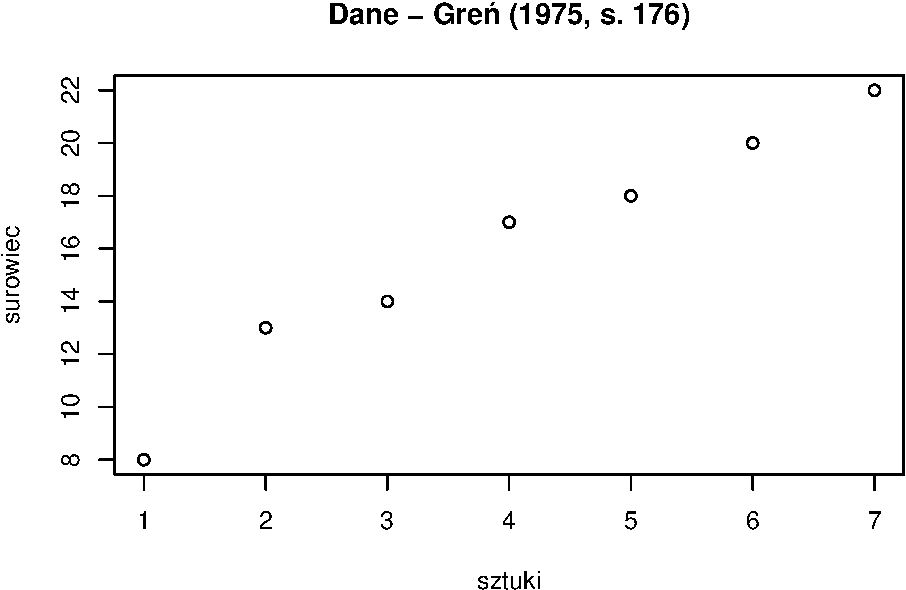
\includegraphics[width=0.7\linewidth]{bookdown-ksiazka_files/figure-latex/unnamed-chunk-115-1} 

}

\caption{Zależność między wielkością produkcji pewnego wyrobu, a zużyciem pewnego surowca}\label{fig:unnamed-chunk-115}
\end{figure}

\begin{verbatim}
> # model: y = a + bx
> # model: surowiec=a+b*sztuki
> # a = (Intercept), czyli wyraz wolny, b = współczynnik regresji
> # wyznaczanie równania regresji liniowej
> model1=lm(surowiec~sztuki)
> summary(model1)
\end{verbatim}

\begin{verbatim}

Call:
lm(formula = surowiec ~ sztuki)

Residuals:
      1       2       3       4       5       6       7 
-1.5714  1.2857  0.1429  1.0000 -0.1429 -0.2857 -0.4286 

Coefficients:
            Estimate Std. Error t value Pr(>|t|)    
(Intercept)   7.4286     0.8806   8.436 0.000384 ***
sztuki        2.1429     0.1969  10.882 0.000114 ***
---
Signif. codes:  0 '***' 0.001 '**' 0.01 '*' 0.05 '.' 0.1 ' ' 1

Residual standard error: 1.042 on 5 degrees of freedom
Multiple R-squared:  0.9595,    Adjusted R-squared:  0.9514 
F-statistic: 118.4 on 1 and 5 DF,  p-value: 0.0001138
\end{verbatim}

\begin{Shaded}
\begin{Highlighting}[]
\KeywordTok{abline}\NormalTok{(model1)  }\CommentTok{# Rys. 7.2}
\end{Highlighting}
\end{Shaded}

\begin{figure}

{\centering 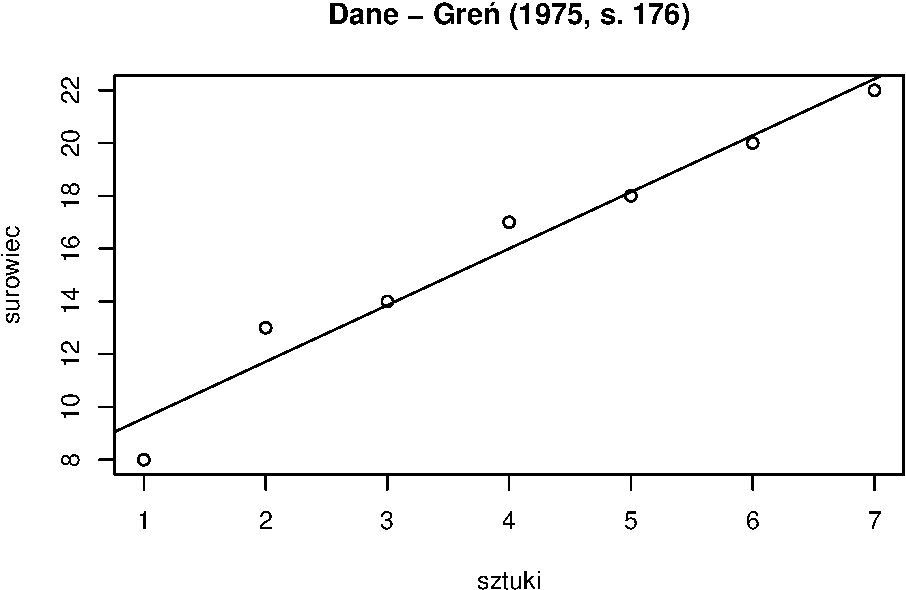
\includegraphics[width=0.7\linewidth]{bookdown-ksiazka_files/figure-latex/unnamed-chunk-117-1} 

}

\caption{Prosta regresji liniowej dla zależności między wielkością produkcji pewnego wyrobu, a zużyciem pewnego surowca}\label{fig:unnamed-chunk-117}
\end{figure}

\vspace{0.8cm} \textbf{Interpretacja}

Ponieważ \(p\)-wartości dla wyrazu wolnego a (Intercept) oraz dla
współczynnika kierunkowego b są mniejsze od 0,05, więc odrzucamy
hipotezy zerowe i przyjmujemy hipotezy alternatywne. Wyraz wolny \(a\)
(Intercept) oraz współczynnik kierunkowy \(b\) są istotne statystycznie
(\(p\)-wartość = 0.000384 oraz \(p\)-wartość = 0.000114, odpowiednio)
dla równania regresji liniowej \(y =a+bx\). Wartość \(R^2=0.9595\)
oznacza, że stopień dopasowania prostej regresji do danych wynosi 96 \%.
Oszacowanie równania regresji liniowej jest postaci:
\(\widehat{surowiec} = 7.4286 + 2.1429 * \textrm{sztuki}\).

\vspace{0.8cm} \textbf{Przykład 7.2} (Kala 2005, s. 94)

W badaniach nad szybkością oddawania wody przez blaszki liściowe pewnego
gatunku trawy poszukiwano w szczególności związku pomiędzy masą
początkową blaszek liściowych bezpośrednio po zerwaniu oraz ich masą po
trzech godzinach przechowywania bez dostępu wody. Dla 10 blaszek
uzyskano obserwacje (w g):

0h: 0.25, 0.33, 0.39, 0.23, 0.19, 0.51, 0.31, 0.24, 0.33, 0.41

3h: 0.09, 0.15, 0.23, 0.10, 0.08, 0.28, 0.17, 0.11, 0.19, 0.24

Wyznaczyć regresję liniową masy blaszki liściowej po trzech godzinach
przechowywania w zależności od masy początkowej.

\vspace{0.8cm} \textbf{Kod w R}

\begin{verbatim}
# Przykład 7.2 (Kala 2005, s. 94)
rm(list = ls())  # usuwanie wszystkich zmiennych z przestrzeni roboczej
# tworzenie danych
h0 = c(0.25, 0.33, 0.39, 0.23, 0.19, 0.51, 0.31, 0.24, 0.33, 0.41)
h3 = c(0.09, 0.15, 0.23, 0.1, 0.08, 0.28, 0.17, 0.11, 0.19, 0.24)
# wykres danych
plot(h0, h3, main = "Dane - Kala (2005, s. 94)", xlab = "masa początkowa blaszek 
     liściowych", 
    ylab = "masa po 3 h blaszek liściowych")  # Rys. 7.3
# wyznaczanie równania regresji liniowej
model2 = lm(h3 ~ h0)
summary(model2)
# na wykresie danych wyznaczana jest prosta regresji
abline(model2)
\end{verbatim}

\vspace{0.8cm} \textbf{Realizacja w R}

\begin{verbatim}
> # Przykład 7.2 (Kala 2005, s. 94)
> rm(list = ls())  # usuwanie wszystkich zmiennych z przestrzeni roboczej
> # tworzenie danych
> h0 = c(0.25, 0.33, 0.39, 0.23, 0.19, 0.51, 0.31, 
+     0.24, 0.33, 0.41)
> h3 = c(0.09, 0.15, 0.23, 0.1, 0.08, 0.28, 0.17, 
+     0.11, 0.19, 0.24)
\end{verbatim}

\begin{verbatim}
> # wykres danych
> plot(h0, h3, main = "Dane - Kala (2005, s. 94)", 
+     xlab = "masa początkowa blaszek liściowych", 
+     ylab = "masa po 3 h blaszek liściowych")  # Rys. 7.3
\end{verbatim}

\begin{figure}[H]

{\centering 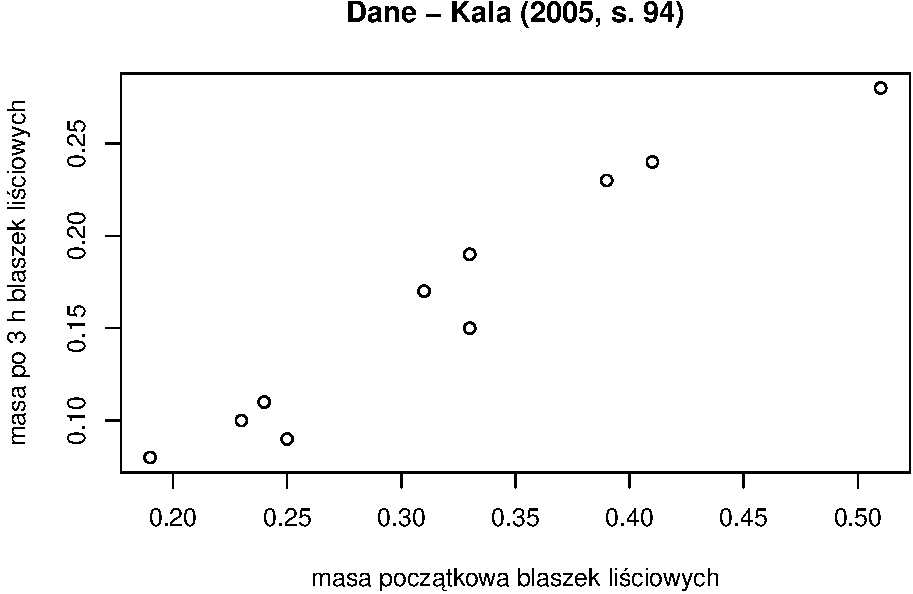
\includegraphics[width=0.7\linewidth]{bookdown-ksiazka_files/figure-latex/unnamed-chunk-120-1} 

}

\caption{Masa blaszki liściowej po trzech godzinach przechowywania w zależności od masy początkowej}\label{fig:unnamed-chunk-120}
\end{figure}

\begin{verbatim}
> # wyznaczanie równania regresji liniowej
> model2 = lm(h3 ~ h0)
> summary(model2)
\end{verbatim}

\begin{verbatim}

Call:
lm(formula = h3 ~ h0)

Residuals:
      Min        1Q    Median        3Q       Max 
-0.025896 -0.013357  0.003505  0.012487  0.018331 

Coefficients:
            Estimate Std. Error t value Pr(>|t|)    
(Intercept) -0.05840    0.01962  -2.977   0.0177 *  
h0           0.69716    0.05906  11.804 2.43e-06 ***
---
Signif. codes:  0 '***' 0.001 '**' 0.01 '*' 0.05 '.' 0.1 ' ' 1

Residual standard error: 0.01729 on 8 degrees of freedom
Multiple R-squared:  0.9457,    Adjusted R-squared:  0.9389 
F-statistic: 139.3 on 1 and 8 DF,  p-value: 2.431e-06
\end{verbatim}

\begin{verbatim}
> # na wykresie danych wyznaczana jest prosta regresji
> abline(model2)
\end{verbatim}

\begin{figure}[H]

{\centering 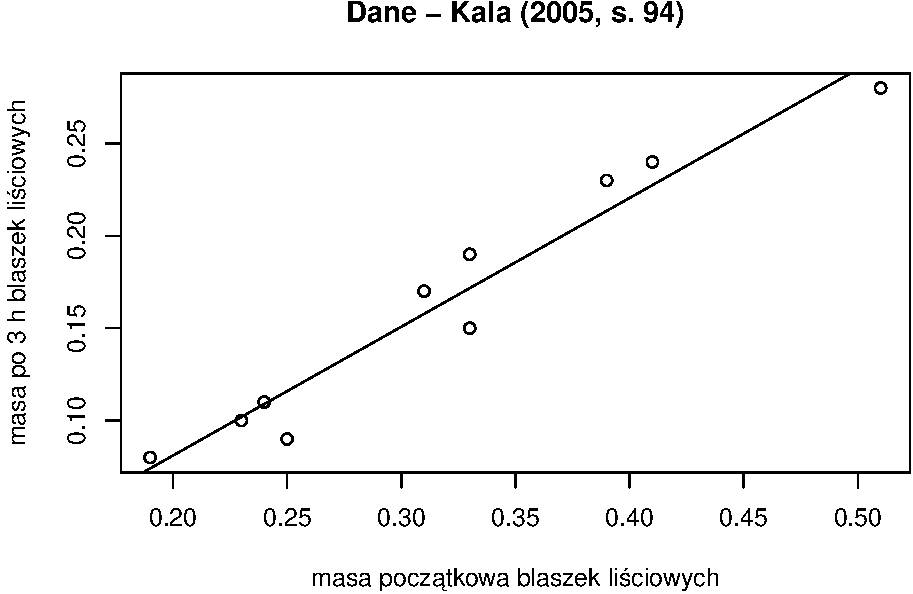
\includegraphics[width=0.7\linewidth]{bookdown-ksiazka_files/figure-latex/unnamed-chunk-122-1} 

}

\caption{Masa blaszki liściowej po trzech godzinach przechowywania w zależności od masy początkowej}\label{fig:unnamed-chunk-122}
\end{figure}

\vspace{0.8cm}

\textbf{Interpretacja}

Ponieważ \(p\)-wartości dla wyrazu wolnego a (Intercept) oraz dla
współczynnika kierunkowego b są mniejsze od 0,05, więc odrzucamy
hipotezy zerowe i przyjmujemy hipotezy alternatywne. Wyraz wolny \(a\)
(Intercept) oraz współczynnik kierunkowy \(b\) są istotne statystycznie
dla równania regresji liniowej \(y =a+bx\) oraz stopień dopasowania
prostej regresji do danych wynosi 94 \%.

Oszacowanie prostej regresji jest postaci: \(\hat{y}= -0.058 + 0.697x\).

\section{Regresja wielokrotna}\label{regresja-wielokrotna}

Mamy dane zmienne niezależne (cechy) \(x_1, x_2, ..., x_n\) i zmienną
zależną \(y\). Chcemy określić zależność liniową pomiędzy zmienną y a
zmiennymi \(x_1, x_2, ..., x_n\), tzn. wyznaczyć liniowy wpływ zmiennych
\(x_1, x_2, ..., x_n\) na zmienną \(y\). W tym celu wyznaczymy regresję
wielokrotną postaci
\(y = b_0 + b_1*x_1 + b_2*x_2 + b_3*x_3 + ... + b_n*x_n\) gdzie:

\(y\) - zmienna zależna, objaśniana (the response variable),
\(x_1, x_2, ..., x_n\) - zmienne niezależne, objaśniające (the predyctor
variables), \(b_0\) - wyraz wolny (Intercept), \(b_1, ..., b_n\) -
współczynniki regresji.

\vspace{0.8cm} Miarą dopasowania regresji wielokrotnej do danych jest
współczynnik determinacji \(R^2\).

W R wyznaczenie regresji wielokrotnej, tak jak regresji liniowej, można
wykonać za pomocą funkcji postaci \texttt{$lm(y \sim x_1+x_2+...+x_n)$}
lub \texttt{$lm(y \sim x_1+x_2+...+x_n, dane)$}.

\vspace{0.8cm} \textbf{Przykład 7.3} (Elandt 1964, s. 441)

Badano cztery cechy słomy konopi: ciężar włókna (g), długość łodygi
(cm), grubość łodygi (mm) oraz ciężar łodygi (g) (Tablica \ref{elandt}).
Znaleźć równanie regresji wielokrotnej liniowej określającej zależność
ciężaru włókna od długości, grubości oraz ciężaru łodygi.

\begin{table}[H]
\centering
\caption{Ciężar włókna  (g), długość łodygi (cm), grubość łodygi (mm) oraz ciężar łodygi  (g) konopi}
\label{elandt}
\begin{tabular}{ccccc|ccccc}
\hline
\multirow{2}{*}{Lp.} & \begin{tabular}[c]{@{}c@{}}ciężar \\ włókna\end{tabular} & \begin{tabular}[c]{@{}c@{}}długość \\ łodygi\end{tabular} & \begin{tabular}[c]{@{}c@{}}grubość\\  łodygi\end{tabular} & \begin{tabular}[c]{@{}c@{}}ciężar\\  łodygi\end{tabular} & \multirow{2}{*}{Lp.} & \begin{tabular}[c]{@{}c@{}}ciężar \\ włókna\end{tabular} & \begin{tabular}[c]{@{}c@{}}długość\\  łodygi\end{tabular} & \begin{tabular}[c]{@{}c@{}}grubość\\  łodygi\end{tabular} & \begin{tabular}[c]{@{}c@{}}ciężar\\  łodygi\end{tabular} \\ \hline
 & y    & x1    & x2  & x3  &                      & y                                                        & x1                                                        & x2                                                        & x3                                                       \\ \hline
1                    & 7.4                                                      & 251                                                       & 9.25                                                      & 47.5                                                     & 26                   & 8.3                                                      & 248                                                       & 8.75                                                      & 51.2                                                     \\
2                    & 9.2                                                      & 255                                                       & 10.50                                                     & 57.7                                                     & 27                   & 8.5                                                      & 248                                                       & 9.50                                                      & 46.1                                                     \\
3                    & 9.6                                                      & 253                                                       & 9.50                                                      & 47.1                                                     & 28                   & 8.9                                                      & 256                                                       & 9.50                                                      & 46.1                                                     \\
4                    & 6.7                                                      & 242                                                       & 8.50                                                      & 38.8                                                     & 29                   & 6.7                                                      & 246                                                       & 9.00                                                      & 40.1                                                     \\
5                    & 7.8                                                      & 246                                                       & 9.50                                                      & 45.2                                                     & 30                   & 7.6                                                      & 247                                                       & 9.00                                                      & 42.9                                                     \\
6                    & 7.8                                                      & 246                                                       & 10.25                                                     & 49.8                                                     & 31                   & 4.6                                                      & 242                                                       & 8.25                                                      & 34.1                                                     \\
7                    & 6.3                                                      & 243                                                       & 8.75                                                      & 43.4                                                     & 32                   & 6.2                                                      & 247                                                       & 9.00                                                      & 38.8                                                     \\
8                    & 7.6                                                      & 246                                                       & 9.00                                                      & 50.8                                                     & 33                   & 7.0                                                      & 250                                                       & 9.25                                                      & 41.5                                                     \\
9                    & 6.4                                                      & 249                                                       & 9.00                                                      & 41.5                                                     & 34                   & 8.9                                                      & 280                                                       & 10.25                                                     & 69.2                                                     \\
10                   & 7.0                                                      & 247                                                       & 9.50                                                      & 38.8                                                     & 35                   & 6.9                                                      & 240                                                       & 9.25                                                      & 43.8                                                     \\
11                   & 6.6                                                      & 237                                                       & 9.75                                                      & 47.1                                                     & 36                   & 8.7                                                      & 243                                                       & 9.25                                                      & 48.9                                                     \\
12                   & 8.2                                                      & 246                                                       & 9.50                                                      & 51.2                                                     & 37                   & 8.5                                                      & 229                                                       & 9.00                                                      & 44.3                                                     \\
13                   & 8.2                                                      & 257                                                       & 9.50                                                      & 52.6                                                     & 38                   & 10.4                                                     & 271                                                       & 9.50                                                      & 52.6                                                     \\
14                   & 7.0                                                      & 250                                                       & 8.75                                                      & 46.1                                                     & 39                   & 8.5                                                      & 266                                                       & 10.50                                                     & 54.5                                                     \\
15                   & 6.8                                                      & 235                                                       & 8.00                                                      & 36.0                                                     & 40                   & 9.8                                                      & 267                                                       & 9.25                                                      & 52.6                                                     \\
16                   & 6.8                                                      & 247                                                       & 10.00                                                     & 44.8                                                     & 41                   & 7.8                                                      & 260                                                       & 8.75                                                      & 51.7                                                     \\
17                   & 9.7                                                      & 234                                                       & 9.50                                                      & 47.1                                                     & 42                   & 7.3                                                      & 247                                                       & 8.75                                                      & 41.5                                                     \\
18                   & 9.3                                                      & 259                                                       & 10.50                                                     & 68.3                                                     & 43                   & 7.0                                                      & 242                                                       & 8.50                                                      & 49.4                                                     \\
19                   & 12.0                                                     & 255                                                       & 10.25                                                     & 62.8                                                     & 44                   & 9.8                                                      & 254                                                       & 10.50                                                     & 59.1                                                     \\
20                   & 8.4                                                      & 264                                                       & 8.50                                                      & 45.7                                                     & 45                   & 8.9                                                      & 262                                                       & 9.50                                                      & 51.7                                                     \\
21                   & 9.5                                                      & 261                                                       & 10.75                                                     & 60.9                                                     & 46                   & 10.2                                                     & 260                                                       & 10.50                                                     & 63.2                                                     \\
22                   & 9.0                                                      & 242                                                       & 9.50                                                      & 45.2                                                     & 47                   & 8.7                                                      & 254                                                       & 8.50                                                      & 51.2                                                     \\
23                   & 6.8                                                      & 240                                                       & 8.25                                                      & 37.8                                                     & 48                   & 6.8                                                      & 249                                                       & 8.75                                                      & 39.7                                                     \\
24                   & 7.3                                                      & 235                                                       & 10.25                                                     & 48.0                                                     & 49                   & 7.5                                                      & 244                                                       & 9.00                                                      & 44.3                                                     \\
25                   & 7.0                                                      & 245                                                       & 8.75                                                      & 44.3                                                     &                      &                                                          &                                                           &                                                           &   \\ \hline                                                      
\end{tabular}
\end{table}

\vspace{0.8cm} \textbf{Kod w R}

\begin{verbatim}
# Przykład 7.3 (Elandt 1964, s. 441)
rm(list=ls()) # usuwanie wszystkich zmiennych z przestrzeni roboczej
# tworzenie danych
sloma=read.table("~/Desktop/Elandt-441-regresja-wielokrotna.txt", header=T)
head(sloma)
# korelacje
round(cor(sloma),2)
# regresja liniowa wielokrotna
regresja=lm(ciezwlokna~dluglodygi+grublodygi+ciezlodygi, data=sloma)
summary(regresja)
\end{verbatim}

\vspace{0.8cm} \textbf{Realizacja w R}

\begin{verbatim}
> # Przykład 7.3 (Elandt 1964, s. 441)
> rm(list=ls()) # usuwanie wszystkich zmiennych z przestrzeni roboczej
> # tworzenie danych
> sloma=read.table("~/Desktop/Elandt-441-regresja-wielokrotna.txt", header=T)
> head(sloma)
\end{verbatim}

\begin{verbatim}
  ciezwlokna dluglodygi grublodygi ciezlodygi
1        7.4        251       9.25       47.5
2        9.2        255      10.50       57.7
3        9.6        253       9.50       47.1
4        6.7        242       8.50       38.8
5        7.8        246       9.50       45.2
6        7.8        246      10.25       49.8
\end{verbatim}

\begin{verbatim}
> # korelacje
> round(cor(sloma),2)
\end{verbatim}

\begin{verbatim}
           ciezwlokna dluglodygi grublodygi ciezlodygi
ciezwlokna       1.00       0.51       0.59       0.75
dluglodygi       0.51       1.00       0.39       0.64
grublodygi       0.59       0.39       1.00       0.73
ciezlodygi       0.75       0.64       0.73       1.00
\end{verbatim}

\vspace{0.8cm}

\textbf{Interpretacja}

Powyżej przedstawione są współczynniki korelacji pomiędzy analizowanymi
zmiennymi tzn. ciężarem włókna, długością łodygi, grubością łodygi i
ciężarem łodygi.

\vspace{0.8cm}

\begin{Shaded}
\begin{Highlighting}[]
\OperatorTok{>}\StringTok{ }\CommentTok{# regresja liniowa wielokrotna}
\ErrorTok{>}\StringTok{ }\NormalTok{regresja=}\KeywordTok{lm}\NormalTok{(ciezwlokna}\OperatorTok{~}\NormalTok{dluglodygi}\OperatorTok{+}\NormalTok{grublodygi}\OperatorTok{+}\NormalTok{ciezlodygi, }\DataTypeTok{data=}\NormalTok{sloma)}
\OperatorTok{>}\StringTok{ }\KeywordTok{summary}\NormalTok{(regresja)}
\end{Highlighting}
\end{Shaded}

\begin{verbatim}

Call:
lm(formula = ciezwlokna ~ dluglodygi + grublodygi + ciezlodygi, 
    data = sloma)

Residuals:
    Min      1Q  Median      3Q     Max 
-1.8650 -0.5898 -0.1117  0.4528  2.1508 

Coefficients:
             Estimate Std. Error t value Pr(>|t|)    
(Intercept) -0.855915   4.398332  -0.195 0.846582    
dluglodygi   0.007644   0.017509   0.437 0.664498    
grublodygi   0.160398   0.285718   0.561 0.577321    
ciezlodygi   0.113245   0.030308   3.736 0.000524 ***
---
Signif. codes:  0 '***' 0.001 '**' 0.01 '*' 0.05 '.' 0.1 ' ' 1

Residual standard error: 0.9233 on 45 degrees of freedom
Multiple R-squared:  0.569, Adjusted R-squared:  0.5402 
F-statistic:  19.8 on 3 and 45 DF,  p-value: 2.492e-08
\end{verbatim}

\vspace{0.4cm}

\textbf{Interpretacja}

Oszacowanie równania regresji liniowej wielokrotnej jest postaci:

\(\widehat{ciezar wlokna} = -0.856+0.008*\textrm{dlugosc lodygi} + 0.16*\textrm{grubosc lodygi}+0.113*\textrm{ciezar lodygi}\)

Współczynnik determinacji wynosi \(R^2=0,569\).

\section{Selekcja zmiennych}\label{selekcja-zmiennych}

Analizując przykład 7.3, po wyznaczeniu równania regresji liniowej
wielokrotnej i otrzymaniu charakterystyk współczynników regresji należy
zauważyć, że p-wartości dla wyrazu wolnego, długości i grubości łodygi
są większe od 0,05 (0.8465882, 0.664498 oraz 0.577321, odpowiednio).
Oznacza to, że długość i grubość łodygi nie mają istotnego wpływu na
ciężar włókna. Skoro tak, to zmienne te (zmienne nieistotne) można nie
uwzględniać w wyznaczaniu równania regresji liniowej wielokrotnej.
Obecnie wyznaczymy równania regresji uwzględniającej tylko ciężar łodygi
jako zmienną niezależną, czyli wyznaczymy równania regresji liniowej.
Takie postępowanie jest jedną z metod selekcji zmiennych. Drugą metodą
jest automatyczna selekcja zmiennych przy pomocy funkcji \texttt{step}.
Program sam dokona selekcji zmiennych. Jest to tzw. selekcja zstępująca.

\vspace{0.8cm} \textbf{Kod w R}

\begin{verbatim}
# cd. przykładu 7.3
regresja1=lm(ciezwlokna~ciezlodygi, data=sloma)
summary(regresja1)
# step()
modelstep=step(regresja)
summary(modelstep)
\end{verbatim}

\vspace{0.8cm} \textbf{Realizacja w R}

\begin{verbatim}
> # cd. przykładu 7.3
> regresja1=lm(ciezwlokna~ciezlodygi, data=sloma)
> summary(regresja1)
\end{verbatim}

\begin{verbatim}

Call:
lm(formula = ciezwlokna ~ ciezlodygi, data = sloma)

Residuals:
    Min      1Q  Median      3Q     Max 
-1.8395 -0.5892 -0.1005  0.3746  2.0922 

Coefficients:
            Estimate Std. Error t value Pr(>|t|)    
(Intercept)  1.74744    0.81087   2.155   0.0363 *  
ciezlodygi   0.12994    0.01664   7.809 4.92e-10 ***
---
Signif. codes:  0 '***' 0.001 '**' 0.01 '*' 0.05 '.' 0.1 ' ' 1

Residual standard error: 0.9078 on 47 degrees of freedom
Multiple R-squared:  0.5647,    Adjusted R-squared:  0.5555 
F-statistic: 60.98 on 1 and 47 DF,  p-value: 4.919e-10
\end{verbatim}

\vspace{0.8cm} \textbf{Interpretacja}

Równanie regresji liniowej wielokrotnej jest postaci:

\(\textrm{ciężar włókna} = 1.74744 + 0.12994*\textrm{ciężar łodygi}\).

Współczynnik determinacji jest równy \(R^2=0.5647\).

\vspace{0.8cm} \textbf{Realizacja w R (c.d.)}

\begin{verbatim}
> # step()
> modelstep=step(regresja)
\end{verbatim}

\begin{verbatim}
Start:  AIC=-4
ciezwlokna ~ dluglodygi + grublodygi + ciezlodygi

             Df Sum of Sq    RSS     AIC
- dluglodygi  1    0.1625 38.520 -5.7911
- grublodygi  1    0.2686 38.627 -5.6562
<none>                    38.358 -3.9982
- ciezlodygi  1   11.9004 50.258  7.2424

Step:  AIC=-5.79
ciezwlokna ~ grublodygi + ciezlodygi

             Df Sum of Sq    RSS     AIC
- grublodygi  1     0.214 38.734 -7.5196
<none>                    38.520 -5.7911
- ciezlodygi  1    20.001 58.521 12.7006

Step:  AIC=-7.52
ciezwlokna ~ ciezlodygi

             Df Sum of Sq    RSS     AIC
<none>                    38.734 -7.5196
- ciezlodygi  1    50.255 88.990 31.2384
\end{verbatim}

\begin{verbatim}
> summary(modelstep)
\end{verbatim}

\begin{verbatim}

Call:
lm(formula = ciezwlokna ~ ciezlodygi, data = sloma)

Residuals:
    Min      1Q  Median      3Q     Max 
-1.8395 -0.5892 -0.1005  0.3746  2.0922 

Coefficients:
            Estimate Std. Error t value Pr(>|t|)    
(Intercept)  1.74744    0.81087   2.155   0.0363 *  
ciezlodygi   0.12994    0.01664   7.809 4.92e-10 ***
---
Signif. codes:  0 '***' 0.001 '**' 0.01 '*' 0.05 '.' 0.1 ' ' 1

Residual standard error: 0.9078 on 47 degrees of freedom
Multiple R-squared:  0.5647,    Adjusted R-squared:  0.5555 
F-statistic: 60.98 on 1 and 47 DF,  p-value: 4.919e-10
\end{verbatim}

\vspace{0.8cm} \textbf{Interpretacja}

Najlepiej dopasowanym równaniem regresji do analizowanych danych jest
równanie z najmniejszą wartością współczynnika Akaike (AIC). Z
powyższych danych wynika, że jest to ostatnie równanie, czyli równanie
regresji liniowej postaci:

\(\textrm{ciężar włókna} = 1.74744 + 0.12994*\textrm{ciężar łodygi}\)

Ponadto, dla tego równania wyraz wolny oraz współczynnik kierunkowy są
istotne statystycznie. Współczynnik determinacji jest równy
\(R^2=0.5647\).

\newpage

\section{Zadania do wykonania}\label{zadania-do-wykonania-6}

\textbf{Regresja liniowa}

Zad. 1 (Greń 1975, s. 179)

Dokonano w pewnej miejscowości 6 pomiarów temperatury dla różnych
głębokości pod powierzchnią ziemi. Otrzymano następujące wyniki (\(x_i\)
głębokość w m, \(y_i\) temperatura w stopniach C):

\(x_i\): 200, 400, 600, 800, 1000, 1200

\(y_i\): 10, 15, 23, 26, 33, 37

Znaleźć równanie regresji liniowej określającej zależność temperatury od
głębokości.

\vspace{0.8cm} \textbf{Regresja wielokrotna}

Zad. 1 (Greń 1975, s. 210)

W pewnym eksperymencie rolniczym zastosowano różne dawki dwu nawozów na
poletkach doświadczalnych i otrzymano następujące dane dotyczące
wysokości uzyskanych plonów (w q/ha) pewnej rośliny uprawnej (\(X_1\)
dawki nawozu A, \(X_2\) dawki nawozu B, \(Y\) wielkość plonu):

\begin{table}[H]
\centering
\caption{Dane - Greń (1975, s. 210)}
\label{gren210}
\begin{tabular}{ccc}
X1 & X2 & Y  \\
1  & 0  & 3  \\
0  & 1  & 7  \\
1  & 1  & 8  \\
2  & 1  & 11 \\
1  & 2  & 14 \\
2  & 2  & 16
\end{tabular}
\end{table}

Oszacować współczynniki regresji wielokrotnej oraz współczynnik
korelacji wielorakiej.

\vspace{0.8cm} \textbf{Selekcja zmiennych}

Zad. 1 (Kala 2005, s. 113)

Badając pewien ród pszenżyta jarego, zmierzono u 10 roślin następujące
cechy: długość kłosa głównego (w cm), liczbę ziarniaków w kłosie głównym
(w szt.), masę ziarniaków z całej rośliny (w g). Uzyskano pomiary:

długość: 10.8, 11.7, 10.3, 11.2, 10, 10.8, 10.6, 10.7, 9.8, 11.5

ziarniaki: 39, 56, 46, 48, 36, 36, 40, 42, 38, 42

masa: 6.7, 7.3, 6, 6.6, 5.4, 6, 5.8, 6.4, 6.1, 6.9

Wyznaczyć równanie regresji wielokrotnej dla masy w zależności od
długości i liczby ziarniaków kłosa głównego oraz wykonać selekcję
zmiennych.

\chapter{Odpowiedzi do zadań}\label{odpowiedzi-do-zadan}

\textbf{Rozdział 1}

Zad. 1

\begin{verbatim}
install.packages('agricolae')
library('agricolae')
?correlation
\end{verbatim}

Zad. 2

\begin{verbatim}
install.packages('agridat')
library('agridat')
??yates.oats
\end{verbatim}

Zad. 3

\begin{verbatim}
install.packages('openxlsx')
library('openxlsx')
?read.xlsx
\end{verbatim}

\newpage

\textbf{Rozdział 2}

\textbf{Wektory}

Zad. 2

\begin{verbatim}
cc<-rep(1,8)
d<-rep(0,199)
\end{verbatim}

Zad. 3

\begin{verbatim}
a)
sum((100:200)^2)
b)
sum(sqrt(log10(10^(0:5)))) 
\end{verbatim}

Zad. 4

\begin{verbatim}
a)
rep(1,8)
b)
rep(c(1,4),7) 
c)
rep(c(3,6),c(8,3))
d)
rep(5:1,1:5)
e)
rep(c(12,21,43),c(3,1,2)) 
f)
rep(c("A","B"),3)
g)
rep(c(1,3,5,7,9,11),each=2)
\end{verbatim}

\newpage

\textbf{Macierze}

Zad. 1

\begin{verbatim}
A=matrix(c(1,2,3,0,2,-5,7,1,-3,4,5,6,0,1,-2,-3),4,4)
B=matrix(c(1,4,3,2,7,2,-1,0),4,2)
det(A)
A%*%B
t(A)
solve(A)
\end{verbatim}

Zad. 2

\begin{verbatim}
A =matrix(c(1,4,7,2,5,8,3,68,9),3,3,byrow=T)
nrow(A)
ncol(A)
sum(A)
colMeans(A)
sum(A[2,])
A[1,2]+A[3,3]
A[,3]
A[2,]
\end{verbatim}

\vspace{0.4cm} \textbf{Ramki danych}

Zad. 1

\begin{verbatim}
data(iris)
dim(iris)
by(iris$Sepal.Width,iris$Species,mean)
by(iris$Sepal.Width,iris$Species,sd)
virginica<-subset(iris,iris$Species=='virginica')
virginica.sl<-virginica$Sepal.Length
table(iris$Species)
by(iris$Sepal.Length,iris$Species,min)
\end{verbatim}

\vspace{0.8cm} \textbf{Rozdział 3}

Zad. 1

\begin{verbatim}
a)
dane<-read.table('dane.txt', header=T)
b)
table(dane$miejsce.zamieszkania)
c)
table(dane$miejsce.zamieszkania,dane$wielkość.rodziny)
d)
table(dane$miejsce.zamieszkania,dane$jedzie.na.wakacje)
e)
max(subset(dane$dochód,dane$wielkość.rodziny=='duże' & 
             dane$miejsce.zamieszkania=='miasto'))
\end{verbatim}

Zad. 2

\begin{verbatim}
library(openxlsx)
dane<-read.xlsx('studenci.xlsx')
a)
table(dane$`Kierunek studiów`,dane$Płeć)
b)
by(dane$`Stypendium naukowe`,dane$Płeć,mean)
c)
subset(dane,dane$Płeć=='kobieta' & dane$`Kierunek studiów`=='Agroturystyka')
d)
subset(dane,dane$`Kierunek studiów`=='Leśnictwo' & dane$Płeć=='mężczyzna' 
       & dane$`Stypendium naukowe`=='0')
\end{verbatim}

\newpage

\textbf{Rozdział 4}

Zad. 1

\begin{verbatim}
library(openxlsx)
dane<-read.xlsx('studenci.xlsx')
plot(dane$Wiek,dane$`Stypendium naukowe`, col=c('red','blue'))
\end{verbatim}

Zad. 2

\begin{verbatim}
curve(x^2,from=-5,to=5,col='red')
curve((x-2)^2,from=-5,to=5,col='orange',add=T)
curve((x-2)^2+3,from=-5,to=5,col='green',add=T)
curve(x^2+3,from=-5,to=5,col='blue',add=T)
curve((x+1)^2-2,from=-5,to=5,col='violet',add=T)
abline(v=0,col='black')
title(main="Wykresy funkcji przesuniętych")
\end{verbatim}

Zad. 3

\begin{verbatim}
hist(dane$`Stypendium naukowe`, main = "Histogram wysokości stypendium
     naukowego", 
    xlab = "Wysokość stypendium naukowego")
\end{verbatim}

\vspace{0.8cm} \textbf{Rozdział 5}

\textbf{Testy dwóch wartości średnich z rozkładów normalnych - próby
zależne}

Zad. 1

\begin{verbatim}
numer_odmiany = 1:4
dł_słomy_1948 = c(68.9, 52.6, 59.5, 60.3)
dł_słomy_1949 = c(64.5, 54.8, 57.9, 57.2)
dane_dł_słomy = data.frame(numer_odmiany, dł_słomy_1948, dł_słomy_1949)
# testowanie zgodności z rozkładem normalnym
shapiro.test(dł_słomy_1948)
shapiro.test(dł_słomy_1949)
dane <- data.frame(Wartości = c(dł_słomy_1948, dł_słomy_1949), Rok = rep(1948:1949, 
    c(4, 4)))
# sprawdzenie równosci wartości średnich
t.test(Wartości ~ Rok, dane, var.equal = TRUE, paired = TRUE, conf.level = 0.95)
\end{verbatim}

Zad. 2

\begin{verbatim}
krzyzowanie <- c(188, 101, 156, 197, 97, 94, 120, 178)
samopylnosc <- c(150, 97, 134, 139, 95, 91, 118, 161)
shapiro.test(krzyzowanie)
shapiro.test(samopylnosc)
t.test(krzyzowanie, samopylnosc, conf.level = 0.95, paired = TRUE)
\end{verbatim}

\vspace{0.8cm} \textbf{Analiza wariancji - Anova}

Zad. 1

\begin{verbatim}
Plon <- c(290, 286, 266, 270, 301, 270, 264, 277, 445, 450, 413, 448, 454, 442, 
    430, 438, 520, 470, 516, 530, 475, 508, 485, 480, 370, 405, 412, 403, 384, 
    410, 415, 377)
Terminy <- as.factor(rep(1:4, c(8, 8, 8, 8)))
levels(Terminy) <- c("I", "II", "III", "IV")
dane <- data.frame(Plon, Terminy)
model <- lm(Plon ~ Terminy, data = dane)
rozwiazanie = anova(model)
rozwiazanie
\end{verbatim}

Zad. 2

\begin{verbatim}
masa <- c(214.6, 193.1, 189.1, 177.7, 262.3, 235.9, 216.5, 219.1, 221.4, 236.8, 
    227.9, 234.1, 248, 255, 229.6, 242.8)
odmiany <- as.factor(c("S", "L", "A", "D"))
dane <- data.frame(masa, odmiany)
model <- lm(masa ~ odmiany, data = dane)
rozwiazanie = anova(model)
rozwiazanie
\end{verbatim}

\vspace{0.8cm} \textbf{Testy wielokrotne}

Zad. 1

\begin{verbatim}
L1 = c(0.26, 0.28, 0.27, 0.25, 0.19)
L2 = c(0.3, 0.27, 0.26, 0.22, 0.19)
L3 = c(0.26, 0.25, 0.24, 0.22, 0.2)
L4 = c(0.25, 0.23, 0.21, 0.22, 0.21)
L5 = c(0.23, 0.22, 0.22, 0.21, 0.2)
L6 = c(0.21, 0.21, 0.2, 0.2, 0.2)
L7 = c(0.24, 0.22, 0.21, 0.2, 0.18)
fenol = c(L1, L2, L3, L4, L5, L6, L7)
jeziora = as.factor(rep(c("L1", "L2", "L3", "L4", "L5", "L6", "L7"), each = 5))
dane = data.frame(fenol, jeziora)
model = aov(fenol ~ jeziora, dane)
a = HSD.test(model, "jeziora")
a
TukeyHSD(model, "jeziora", ordered = TRUE)
plot(TukeyHSD(model, "jeziora"))
\end{verbatim}

Zad. 2

\begin{verbatim}
plon = c(0.16, 0.18, 0.62, 0.62, 0.29, 0.39, 0.61, 0.23, 0.28, 0.38, 0.68, 0.24, 
    0.37, 0.65, 0.39, 0.39, 0.63, 0.63, 0.2, 0.49, 0.57, 0.34, 0.16, 0.52, 0.52, 
    0.26, 0.44, 0.67, 0.23, 0.48, 0.61, 0.61, 0.18, 0.47, 0.69, 0.38, 0.44, 
    0.57, 0.57, 0.19, 0.53, 0.65)
nawożenie = as.factor(rep(c("K", "N1", "N2", "N3", "N4", "N5", "N6"), 6))
dane <- data.frame(plon, nawożenie)
model = aov(plon ~ nawożenie, dane)
a = HSD.test(model, "nawożenie")
a
TukeyHSD(model, "nawożenie", ordered = TRUE)
plot(TukeyHSD(model, "nawożenie"))
\end{verbatim}

\vspace{0.8cm} \textbf{Rozdział 6} \vspace{0.8cm}

\textbf{Korelacje}

Zad. 1

\begin{verbatim}
wysokość = c(163, 170, 158, 156, 161, 159, 161, 168, 177)
obwód = c(21, 24, 22, 19, 24, 26, 26, 27, 28)
cor.test(wysokość, obwód)
\end{verbatim}

Zad. 2

\begin{verbatim}
masa = c(44.1, 45.6, 45.2, 46.8, 43.3, 47.1, 46.8, 45.7)
plon = c(4.68, 4.76, 4.71, 4.87, 4.31, 4.97, 4.82, 4.72)
cor.test(masa, plon)
\end{verbatim}

\vspace{0.8cm} \textbf{Tablice kontyngencji}

Zad. 1

\begin{verbatim}
x = matrix(c(71, 19, 57, 63), ncol = 2)
x
chisq.test(x)
\end{verbatim}

Zad. 2

\begin{verbatim}
x = matrix(c(18, 25, 31, 183), ncol = 2)
x
chisq.test(x)
\end{verbatim}

\newpage

\textbf{Rozdział 7}

\textbf{Regresja liniowa}

Zad. 1

\begin{verbatim}
x = c(200, 400, 600, 800, 1000, 1200)
y = c(10, 15, 23, 26, 33, 37)
model1=lm(y~x)
summary(model1)
\end{verbatim}

Zad. 2

\begin{verbatim}
X1=c(1,0,1,2,1,2)
X2=c(0,1,1,1,2,2)
Y<-c(3,7,8,11,14,16)
plon = data.frame(X1, X2, Y)
plon
modelw = lm(Y ~ X1 + X2, data = plon)
summary(modelw)
\end{verbatim}

\bibliography{packages.bib,book.bib}


\end{document}
